%********************************************%
%*       Generated from PreTeXt source      *%
%*       on 2025-01-16T15:12:28-05:00       *%
%*   A recent stable commit (2022-07-01):   *%
%* 6c761d3dba23af92cba35001c852aac04ae99a5f *%
%*                                          *%
%*         https://pretextbook.org          *%
%*                                          *%
%********************************************%
\documentclass[twoside,14pt]{extarticle}
%% Custom Preamble Entries, early (use latex.preamble.early)
%% Always open on odd page
%%   The following adjusts cleardoublepage to remove twosided
%%   check so that we open on odd pages even in one-sided mode
%%   by adding an extra blank page on the preceding even page.
\makeatletter%
\def\cleardoublepage{%
\clearpage\ifodd\c@page\else\thispagestyle{empty}\hbox{}\newpage\if@twocolumn\hbox{}\newpage\fi\fi%
}
\makeatother%
%% Default LaTeX packages
%%   1.  always employed (or nearly so) for some purpose, or
%%   2.  a stylewriter may assume their presence
\usepackage{geometry}
%% Some aspects of the preamble are conditional,
%% the LaTeX engine is one such determinant
\usepackage{ifthen}
%% etoolbox has a variety of modern conveniences
\usepackage{etoolbox}
\usepackage{ifxetex,ifluatex}
%% Raster graphics inclusion
\usepackage{graphicx}
%% Color support, xcolor package
%% Always loaded, for: add/delete text, author tools
%% Here, since tcolorbox loads tikz, and tikz loads xcolor
\PassOptionsToPackage{dvipsnames,svgnames,table}{xcolor}
\usepackage{xcolor}
%% begin: defined colors, via xcolor package, for styling
%% end: defined colors, via xcolor package, for styling
%% Colored boxes, and much more, though mostly styling
%% skins library provides "enhanced" skin, employing tikzpicture
%% boxes may be configured as "breakable" or "unbreakable"
%% "raster" controls grids of boxes, aka side-by-side
\usepackage{tcolorbox}
\tcbuselibrary{skins}
\tcbuselibrary{breakable}
\tcbuselibrary{raster}
%% We load some "stock" tcolorbox styles that we use a lot
%% Placement here is provisional, there will be some color work also
%% First, black on white, no border, transparent, but no assumption about titles
\tcbset{ bwminimalstyle/.style={size=minimal, boxrule=-0.3pt, frame empty,
colback=white, colbacktitle=white, coltitle=black, opacityfill=0.0} }
%% Second, bold title, run-in to text/paragraph/heading
%% Space afterwards will be controlled by environment,
%% independent of constructions of the tcb title
%% Places \blocktitlefont onto many block titles
\tcbset{ runintitlestyle/.style={fonttitle=\blocktitlefont\upshape\bfseries, attach title to upper} }
%% Spacing prior to each exercise, anywhere
\tcbset{ exercisespacingstyle/.style={before skip={1.5ex plus 0.5ex}} }
%% Spacing prior to each block
\tcbset{ blockspacingstyle/.style={before skip={2.0ex plus 0.5ex}} }
%% xparse allows the construction of more robust commands,
%% this is a necessity for isolating styling and behavior
%% The tcolorbox library of the same name loads the base library
\tcbuselibrary{xparse}
%% The tcolorbox library loads TikZ, its calc package is generally useful,
%% and is necessary for some smaller documents that use partial tcolor boxes
%% See:  https://github.com/PreTeXtBook/pretext/issues/1624
\usetikzlibrary{calc}
%% We use some more exotic tcolorbox keys to restore indentation to parboxes
\tcbuselibrary{hooks}
%% Save default paragraph indentation and parskip for use later, when adjusting parboxes
\newlength{\normalparindent}
\newlength{\normalparskip}
\AtBeginDocument{\setlength{\normalparindent}{\parindent}}
\AtBeginDocument{\setlength{\normalparskip}{\parskip}}
\newcommand{\setparstyle}{\setlength{\parindent}{\normalparindent}\setlength{\parskip}{\normalparskip}}%% Hyperref should be here, but likes to be loaded late
%%
%% Inline math delimiters, \(, \), need to be robust
%% 2016-01-31:  latexrelease.sty  supersedes  fixltx2e.sty
%% If  latexrelease.sty  exists, bugfix is in kernel
%% If not, bugfix is in  fixltx2e.sty
%% See:  https://tug.org/TUGboat/tb36-3/tb114ltnews22.pdf
%% and read "Fewer fragile commands" in distribution's  latexchanges.pdf
\IfFileExists{latexrelease.sty}{}{\usepackage{fixltx2e}}
%% shorter subnumbers in some side-by-side require manipulations
\usepackage{xstring}
%% Footnote counters and part/chapter counters are manipulated
%% April 2018:  chngcntr  commands now integrated into the kernel,
%% but circa 2018/2019 the package would still try to redefine them,
%% so we need to do the work of loading conditionally for old kernels.
%% From version 1.1a,  chngcntr  should detect defintions made by LaTeX kernel.
\ifdefined\counterwithin
\else
    \usepackage{chngcntr}
\fi
%% Text height identically 9 inches, text width varies on point size
%% See Bringhurst 2.1.1 on measure for recommendations
%% 75 characters per line (count spaces, punctuation) is target
%% which is the upper limit of Bringhurst's recommendations
\geometry{letterpaper, inner=1.5in, outer=1in, top=0.35in, bottom=0.7in}
%% Custom Page Layout Adjustments (use publisher page-geometry entry)
%% This LaTeX file may be compiled with pdflatex, xelatex, or lualatex executables
%% LuaTeX is not explicitly supported, but we do accept additions from knowledgeable users
%% The conditional below provides  pdflatex  specific configuration last
%% begin: engine-specific capabilities
\ifthenelse{\boolean{xetex} \or \boolean{luatex}}{%
%% begin: xelatex and lualatex-specific default configuration
\ifxetex\usepackage{xltxtra}\fi
%% realscripts is the only part of xltxtra relevant to lualatex 
\ifluatex\usepackage{realscripts}\fi
%% end:   xelatex and lualatex-specific default configuration
}{
%% begin: pdflatex-specific default configuration
%% We assume a PreTeXt XML source file may have Unicode characters
%% and so we ask LaTeX to parse a UTF-8 encoded file
%% This may work well for accented characters in Western language,
%% but not with Greek, Asian languages, etc.
%% When this is not good enough, switch to the  xelatex  engine
%% where Unicode is better supported (encouraged, even)
\usepackage[utf8]{inputenc}
%% end: pdflatex-specific default configuration
}
%% end:   engine-specific capabilities
%%
%% Fonts.  Conditional on LaTex engine employed.
%% Default Text Font: The Latin Modern fonts are
%% "enhanced versions of the [original TeX] Computer Modern fonts."
%% We use them as the default text font for PreTeXt output.
%% Automatic Font Control
%% Portions of a document, are, or may, be affected by defined commands
%% These are perhaps more flexible when using  xelatex  rather than  pdflatex
%% The following definitions are meant to be re-defined in a style, using \renewcommand
%% They are scoped when employed (in a TeX group), and so should not be defined with an argument
\newcommand{\divisionfont}{\relax}
\newcommand{\blocktitlefont}{\relax}
\newcommand{\contentsfont}{\relax}
\newcommand{\pagefont}{\relax}
\newcommand{\tabularfont}{\relax}
\newcommand{\xreffont}{\relax}
\newcommand{\titlepagefont}{\relax}
%%
\ifthenelse{\boolean{xetex} \or \boolean{luatex}}{%
%% begin: font setup and configuration for use with xelatex
%% Generally, xelatex is necessary for non-Western fonts
%% fontspec package provides extensive control of system fonts,
%% meaning *.otf (OpenType), and apparently *.ttf (TrueType)
%% that live *outside* your TeX/MF tree, and are controlled by your *system*
%% (it is possible that a TeX distribution will place fonts in a system location)
%%
%% The fontspec package is the best vehicle for using different fonts in  xelatex
%% So we load it always, no matter what a publisher or style might want
%%
\usepackage{fontspec}
%%
%% begin: xelatex main font ("font-xelatex-main" template)
%% Latin Modern Roman is the default font for xelatex and so is loaded with a TU encoding
%% *in the format* so we can't touch it, only perhaps adjust it later
%% in one of two ways (then known by NFSS names such as "lmr")
%% (1) via NFSS with font family names such as "lmr" and "lmss"
%% (2) via fontspec with commands like \setmainfont{Latin Modern Roman}
%% The latter requires the font to be known at the system-level by its font name,
%% but will give access to OTF font features through optional arguments
%% https://tex.stackexchange.com/questions/470008/
%% where-and-how-does-fontspec-sty-specify-the-default-font-latin-modern-roman
%% http://tex.stackexchange.com/questions/115321
%% /how-to-optimize-latin-modern-font-with-xelatex
%%
%% end:   xelatex main font ("font-xelatex-main" template)
%% begin: xelatex mono font ("font-xelatex-mono" template)
%% (conditional on non-trivial uses being present in source)
%% end:   xelatex mono font ("font-xelatex-mono" template)
%% begin: xelatex font adjustments ("font-xelatex-style" template)
%% end:   xelatex font adjustments ("font-xelatex-style" template)
%%
%% Extensive support for other languages
\usepackage{polyglossia}
%% Set main/default language based on pretext/@xml:lang value
%% document language code is "es-ES", Spanish
\setmainlanguage{spanish}
%% Enable secondary languages based on discovery of @xml:lang values
%% Enable fonts/scripts based on discovery of @xml:lang values
%% Western languages should be ably covered by Latin Modern Roman
%% end:   font setup and configuration for use with xelatex
}{%
%% begin: font setup and configuration for use with pdflatex
%% begin: pdflatex main font ("font-pdflatex-main" template)
\usepackage{lmodern}
\usepackage[T1]{fontenc}
%% end:   pdflatex main font ("font-pdflatex-main" template)
%% begin: pdflatex mono font ("font-pdflatex-mono" template)
%% (conditional on non-trivial uses being present in source)
%% end:   pdflatex mono font ("font-pdflatex-mono" template)
%% begin: pdflatex font adjustments ("font-pdflatex-style" template)
%% end:   pdflatex font adjustments ("font-pdflatex-style" template)
%% end:   font setup and configuration for use with pdflatex
}
%% Micromanage spacing, etc.  The named "microtype-options"
%% template may be employed to fine-tune package behavior
\usepackage{microtype}
%% Symbols, align environment, commutative diagrams, bracket-matrix
\usepackage{amsmath}
\usepackage{amscd}
\usepackage{amssymb}
%% allow page breaks within display mathematics anywhere
%% level 4 is maximally permissive
%% this is exactly the opposite of AMSmath package philosophy
%% there are per-display, and per-equation options to control this
%% split, aligned, gathered, and alignedat are not affected
\allowdisplaybreaks[4]
%% allow more columns to a matrix
%% can make this even bigger by overriding with  latex.preamble.late  processing option
\setcounter{MaxMatrixCols}{30}
%%
%%
%% Division Titles, and Page Headers/Footers
%% titlesec package, loading "titleps" package cooperatively
%% See code comments about the necessity and purpose of "explicit" option.
%% The "newparttoc" option causes a consistent entry for parts in the ToC 
%% file, but it is only effective if there is a \titleformat for \part.
%% "pagestyles" loads the  titleps  package cooperatively.
\usepackage[explicit, newparttoc, pagestyles]{titlesec}
%% The companion titletoc package for the ToC.
\usepackage{titletoc}
%% begin: customizations of page styles via the modal "titleps-style" template
%% Designed to use commands from the LaTeX "titleps" package
\pagestyle{plain}
%% end: customizations of page styles via the modal "titleps-style" template
%%
%% Create globally-available macros to be provided for style writers
%% These are redefined for each occurence of each division
\newcommand{\divisionnameptx}{\relax}%
\newcommand{\titleptx}{\relax}%
\newcommand{\subtitleptx}{\relax}%
\newcommand{\shortitleptx}{\relax}%
\newcommand{\authorsptx}{\relax}%
\newcommand{\epigraphptx}{\relax}%
%% Create environments for possible occurences of each division
%% Environment for a PTX "section" at the level of a LaTeX "section"
\NewDocumentEnvironment{sectionptx}{mmmmmmm}
{%
\renewcommand{\divisionnameptx}{#1}%
\renewcommand{\titleptx}{#2}%
\renewcommand{\subtitleptx}{#3}%
\renewcommand{\shortitleptx}{#4}%
\renewcommand{\authorsptx}{#5}%
\renewcommand{\epigraphptx}{#6}%
\clearpage
\section[{#4}]{\LARGE #2}%
\label{#7}%
}{}%
%% Environment for a PTX "subsection" at the level of a LaTeX "subsection"
\NewDocumentEnvironment{subsectionptx}{mmmmmmm}
{%
\renewcommand{\divisionnameptx}{#1}%
\renewcommand{\titleptx}{#2}%
\renewcommand{\subtitleptx}{#3}%
\renewcommand{\shortitleptx}{#4}%
\renewcommand{\authorsptx}{#5}%
\renewcommand{\epigraphptx}{#6}%
\newpage
\subsection[{#4}]{\Large #2}%
\vspace{-0.3cm}%
\label{#7}%
}{}%
%% Environment for a PTX "subsubsection" at the level of a LaTeX "subsubsection"
\NewDocumentEnvironment{subsubsectionptx}{mmmmmmm}
{%
\renewcommand{\divisionnameptx}{#1}%
\renewcommand{\titleptx}{#2}%
\renewcommand{\subtitleptx}{#3}%
\renewcommand{\shortitleptx}{#4}%
\renewcommand{\authorsptx}{#5}%
\renewcommand{\epigraphptx}{#6}%
\vspace{-0.4cm}
\subsubsection[{#4}]{#2}\nobreak%
\vspace{-0.4cm}
\label{#7}%
}{}%
%% Environment for a PTX "exercises" at the level of a LaTeX "subsection"
\NewDocumentEnvironment{exercises-subsection}{mmmmmmm}
{%
\renewcommand{\divisionnameptx}{#1}%
\renewcommand{\titleptx}{#2}%
\renewcommand{\subtitleptx}{#3}%
\renewcommand{\shortitleptx}{#4}%
\renewcommand{\authorsptx}{#5}%
\renewcommand{\epigraphptx}{#6}%
\subsection[{#4}]{#2}%
\label{#7}%
}{}%
%% Environment for a PTX "exercises" at the level of a LaTeX "subsection"
\NewDocumentEnvironment{exercises-subsection-numberless}{mmmmmmm}
{%
\renewcommand{\divisionnameptx}{#1}%
\renewcommand{\titleptx}{#2}%
\renewcommand{\subtitleptx}{#3}%
\renewcommand{\shortitleptx}{#4}%
\renewcommand{\authorsptx}{#5}%
\renewcommand{\epigraphptx}{#6}%
\subsection*{#2}%
\addcontentsline{toc}{subsection}{#4}
\label{#7}%
}{}%
%% Environment for a PTX "references" at the level of a LaTeX "subsection"
\NewDocumentEnvironment{references-subsection}{mmmmmmm}
{%
\renewcommand{\divisionnameptx}{#1}%
\renewcommand{\titleptx}{#2}%
\renewcommand{\subtitleptx}{#3}%
\renewcommand{\shortitleptx}{#4}%
\renewcommand{\authorsptx}{#5}%
\renewcommand{\epigraphptx}{#6}%
\newpage
\subsection[{#4}]{#2}%
\label{#7}%
}{}%
%% Environment for a PTX "references" at the level of a LaTeX "subsection"
\NewDocumentEnvironment{references-subsection-numberless}{mmmmmmm}
{%
\renewcommand{\divisionnameptx}{#1}%
\renewcommand{\titleptx}{#2}%
\renewcommand{\subtitleptx}{#3}%
\renewcommand{\shortitleptx}{#4}%
\renewcommand{\authorsptx}{#5}%
\renewcommand{\epigraphptx}{#6}%
\newpage
\subsection*{#2}%
\addcontentsline{toc}{subsection}{#4}
\label{#7}%
}{}%
%% Environment for a PTX "reading-questions" at the level of a LaTeX "subsubsection"
\NewDocumentEnvironment{reading-questions-subsubsection}{mmmmmmm}
{%
\renewcommand{\divisionnameptx}{#1}%
\renewcommand{\titleptx}{#2}%
\renewcommand{\subtitleptx}{#3}%
\renewcommand{\shortitleptx}{#4}%
\renewcommand{\authorsptx}{#5}%
\renewcommand{\epigraphptx}{#6}%
\vspace{-0.4cm}
\subsubsection[{#4}]{#2}\nobreak%
\vspace{-0.4cm}
\label{#7}%
}{}%
%% Environment for a PTX "reading-questions" at the level of a LaTeX "subsubsection"
\NewDocumentEnvironment{reading-questions-subsubsection-numberless}{mmmmmmm}
{%
\renewcommand{\divisionnameptx}{#1}%
\renewcommand{\titleptx}{#2}%
\renewcommand{\subtitleptx}{#3}%
\renewcommand{\shortitleptx}{#4}%
\renewcommand{\authorsptx}{#5}%
\renewcommand{\epigraphptx}{#6}%
\subsubsection*{#2}\nobreak%
\addcontentsline{toc}{subsubsection}{#4}
\label{#7}%
}{}%
%% Environment for a PTX "references" at the level of a LaTeX "section"
\NewDocumentEnvironment{references-section}{mmmmmmm}
{%
\renewcommand{\divisionnameptx}{#1}%
\renewcommand{\titleptx}{#2}%
\renewcommand{\subtitleptx}{#3}%
\renewcommand{\shortitleptx}{#4}%
\renewcommand{\authorsptx}{#5}%
\renewcommand{\epigraphptx}{#6}%
\section[{#4}]{#2}%
\label{#7}%
}{}%
%% Environment for a PTX "references" at the level of a LaTeX "section"
\NewDocumentEnvironment{references-section-numberless}{mmmmmmm}
{%
\renewcommand{\divisionnameptx}{#1}%
\renewcommand{\titleptx}{#2}%
\renewcommand{\subtitleptx}{#3}%
\renewcommand{\shortitleptx}{#4}%
\renewcommand{\authorsptx}{#5}%
\renewcommand{\epigraphptx}{#6}%
\section*{#2}%
\addcontentsline{toc}{section}{#4}
\label{#7}%
}{}%
%%
%% Styles for six traditional LaTeX divisions
\titleformat{\part}[display]
{\divisionfont\Huge\bfseries\centering}{\divisionnameptx\space\thepart}{30pt}{\Huge#1}
[{\Large\centering\authorsptx}]
\titleformat{\chapter}[display]
{\divisionfont\huge\bfseries}{\divisionnameptx\space\thechapter}{20pt}{\Huge#1}
[{\Large\authorsptx}]
\titleformat{name=\chapter,numberless}[display]
{\divisionfont\huge\bfseries}{}{0pt}{#1}
[{\Large\authorsptx}]
\titlespacing*{\chapter}{0pt}{50pt}{40pt}
\titleformat{\section}[hang]
{\divisionfont\Large\bfseries}{\thesection}{1ex}{#1}
[{\large\authorsptx}]
\titleformat{name=\section,numberless}[block]
{\divisionfont\Large\bfseries}{}{0pt}{#1}
[{\large\authorsptx}]
\titlespacing*{\section}{0pt}{3.5ex plus 1ex minus .2ex}{2.3ex plus .2ex}
\titleformat{\subsection}[hang]
{\divisionfont\large\bfseries}{\thesubsection}{}{#1}
[{\normalsize\authorsptx}]
\titleformat{name=\subsection,numberless}[block]
{\divisionfont\large\bfseries}{}{0pt}{#1}
[{\normalsize\authorsptx}]
\titlespacing*{\subsection}{0pt}{0pt}{0.8ex plus 0.2ex minus 0.1ex}
\titleformat{\subsubsection}[hang]
{\divisionfont\normalsize\bfseries}{\thesubsubsection}{1em}{#1}
[{\small\authorsptx}]
\titleformat{name=\subsubsection,numberless}[block]
{\divisionfont\normalsize\bfseries}{}{0pt}{#1}
[{\normalsize\authorsptx}]
\titlespacing*{\subsubsection}{0pt}{2.5ex plus 0.1ex minus .2ex}{0.5ex plus 0.1ex minus 0.2ex}
\titleformat{\paragraph}[hang]
{\divisionfont\normalsize\bfseries}{\theparagraph}{1em}{#1}
[{\small\authorsptx}]
\titleformat{name=\paragraph,numberless}[block]
{\divisionfont\normalsize\bfseries}{}{0pt}{#1}
[{\normalsize\authorsptx}]
\titlespacing*{\paragraph}{0pt}{3.25ex plus 1ex minus .2ex}{1.5em}
%%
%% Styles for five traditional LaTeX divisions
\titlecontents{part}%
[0pt]{\contentsmargin{0em}\addvspace{1pc}\contentsfont\bfseries}%
{\Large\thecontentslabel\enspace}{\Large}%
{}%
[\addvspace{.5pc}]%
\titlecontents{chapter}%
[0pt]{\contentsmargin{0em}\addvspace{1pc}\contentsfont\bfseries}%
{\large\thecontentslabel\enspace}{\large}%
{\hfill\bfseries\thecontentspage}%
[\addvspace{.5pc}]%
\dottedcontents{section}[3.8em]{\contentsfont}{2.3em}{1pc}%
\dottedcontents{subsection}[6.1em]{\contentsfont}{3.2em}{1pc}%
\dottedcontents{subsubsection}[9.3em]{\contentsfont}{4.3em}{1pc}%
%%
%% Begin: Semantic Macros
%% To preserve meaning in a LaTeX file
%%
%% \mono macro for content of "c", "cd", "tag", etc elements
%% Also used automatically in other constructions
%% Simply an alias for \texttt
%% Always defined, even if there is no need, or if a specific tt font is not loaded
\newcommand{\mono}[1]{\texttt{#1}}
%%
%% Following semantic macros are only defined here if their
%% use is required only in this specific document
%%
%% Used for warnings, typically bold and italic
\newcommand{\alert}[1]{\textbf{\textit{#1}}}
%% Used for fillin answer blank in text
%% Relies on calc package, loaded via tcolorbox
%% Argument is intended number of characters of blank
%% Length may compress for output to fit in one line
\newlength{\fillinmaxwidth}
\newlength{\fillincontract}
\newlength{\charmaxwidth}\setlength{\charmaxwidth}{0.5em}
\newlength{\charminwidth}\setlength{\charminwidth}{0.1em}
\newlength{\fillinheight}
\newcommand{\fillintext}[1]{%
\setlength{\fillinmaxwidth}{#1\charmaxwidth}%
\setlength{\fillincontract}{#1\charminwidth}%
\setlength{\fillinheight}{\baselineskip}\addtolength{\fillinheight}{1.2pt}%
\strut\nobreak\leaders\vbox{\hrule width 0.3pt height 0.3pt \vskip -1.2pt}\hskip 1\fillinmaxwidth minus \fillincontract\nobreak\strut%
}
%% End: Semantic Macros
%% Divisional exercises (and worksheet) as LaTeX environments
%% Third argument is option for extra workspace in worksheets
%% Hanging indent occupies a 5ex width slot prior to left margin
%% Experimentally this seems just barely sufficient for a bold "888."
%% Division exercises, not in exercise group
\tcbset{ divisionexercisestyle/.style={bwminimalstyle, runintitlestyle, exercisespacingstyle, left=5ex, breakable, before upper app={\setlength{\parskip}{\medskipamount}}, } }
\newtcolorbox{divisionexercise}[4]{divisionexercisestyle, before title={\hspace*{-5ex}\makebox[5ex][l]{#1.}}, title={\notblank{#2}{#2}{}}, after title={\space}, phantom={\label{#4}\hypertarget{#4}{}}, after={\notblank{#3}{\newline\rule{\workspacestrutwidth}{#3}\newline\vfill}{\par}}}
%% "tcolorbox" environment for a single image, occupying entire \linewidth
%% arguments are left-margin, width, right-margin, as multiples of
%% \linewidth, and are guaranteed to be positive and sum to 1.0
\tcbset{ imagestyle/.style={bwminimalstyle} }
\NewTColorBox{tcbimage}{mmm}{imagestyle,left skip=#1\linewidth,width=#2\linewidth}
%% Wrapper environment for tcbimage environment with a fourth argument
%% Fourth argument, if nonempty, is a vertical space adjustment
%% and implies image will be preceded by \leavevmode\nopagebreak
%% Intended use is for alignment with a list marker
\NewDocumentEnvironment{image}{mmmm}{\notblank{#4}{\leavevmode\nopagebreak\vspace{#4}}{}\begin{tcbimage}{#1}{#2}{#3}}{\end{tcbimage}%
}%% Footnote Numbering
%% Specified by numbering.footnotes.level
%% Global numbering, since numbering.footnotes.level = 0
%% Multiple column, column-major lists
\usepackage{multicol}
%% More flexible list management, esp. for references
%% But also for specifying labels (i.e. custom order) on nested lists
\usepackage{enumitem}
\setlist{nosep, topsep=0pt, partopsep=0ex, parsep=1ex}
%% Lists of references in their own section, maximum depth 1
\newlist{referencelist}{description}{4}
\setlist[referencelist]{leftmargin=!,labelwidth=!,labelsep=0ex,itemsep=1.0ex,topsep=1.0ex,partopsep=0pt,parsep=0pt}
%% Description lists as tcolorbox sidebyside
%% "dli" short for "description list item"
\newlength{\dlititlewidth}
\newlength{\dlimaxnarrowtitle}\setlength{\dlimaxnarrowtitle}{11ex}
\newlength{\dlimaxmediumtitle}\setlength{\dlimaxmediumtitle}{18ex}
\tcbset{ dlistyle/.style={sidebyside, sidebyside align=top seam, lower separated=false, bwminimalstyle, bottomtitle=0.75ex, after skip=1.5ex, boxsep=0pt, left=0pt, right=0pt, top=0pt, bottom=0pt} }
\tcbset{ dlinarrowstyle/.style={dlistyle, lefthand width=\dlimaxnarrowtitle, sidebyside gap=1ex, halign=flush left, righttitle=10ex} }
\tcbset{ dlimediumstyle/.style={dlistyle, lefthand width=\dlimaxmediumtitle, sidebyside gap=4ex, halign=flush right} }
\NewDocumentEnvironment{descriptionlist}{}{\par\vspace*{1.5ex}}{\par\vspace*{1.5ex}}%
%% begin enviroment has an if/then to open the tcolorbox
\NewDocumentEnvironment{dlinarrow}{mm}{%
\settowidth{\dlititlewidth}{{\textbf{#1}}}%
\ifthenelse{\dlititlewidth > \dlimaxnarrowtitle}%
{\begin{tcolorbox}[title={\textbf{#1}}, phantom={\hypertarget{#2}{}}, dlinarrowstyle]\tcblower}%
{\begin{tcolorbox}[dlinarrowstyle, phantom={\hypertarget{#2}{}}]\textbf{#1}\tcblower}%
}%
{\end{tcolorbox}}%
%% medium option is simpler
\NewDocumentEnvironment{dlimedium}{mm}%
{\begin{tcolorbox}[dlimediumstyle, phantom={\hypertarget{#2}{}}]\textbf{#1}\tcblower}%
{\end{tcolorbox}}%
%% hyperref driver does not need to be specified, it will be detected
%% Footnote marks in tcolorbox have broken linking under
%% hyperref, so it is necessary to turn off all linking
%% It *must* be given as a package option, not with \hypersetup
\usepackage[hyperfootnotes=false]{hyperref}
%% configure hyperref's  \href{}{}  and  \nolinkurl  to match listings' inline verbatim
\renewcommand\UrlFont{\small\ttfamily}
%% For a print PDF, no surrounding boxes, so simply textcolor (but still active to preserve spacing)
\hypersetup{hidelinks}
%% Less-clever names for hyperlinks are more reliable, *especially* for structural parts
%% See comments in the code to learn more about the importance of this setting
\hypersetup{hypertexnames=false}
%%The  hypertexnames  setting then confuses the hyperlinking from the index
%%This patch resolves the incorrect links, see code for StackExchange post.
\makeatletter
\patchcmd\Hy@EveryPageBoxHook{\Hy@EveryPageAnchor}{\Hy@hypertexnamestrue\Hy@EveryPageAnchor}{}{\fail}
\makeatother
\hypersetup{pdftitle={Matemáticas Ilustrativas}}
%% If you manually remove hyperref, leave in this next command
%% This will allow LaTeX compilation, employing this no-op command
\providecommand\phantomsection{}
%% Division Numbering: Chapters, Sections, Subsections, etc
%% Division numbers may be turned off at some level ("depth")
%% A section *always* has depth 1, contrary to us counting from the document root
%% The latex default is 3.  If a larger number is present here, then
%% removing this command may make some cross-references ambiguous
%% The precursor variable $numbering-maxlevel is checked for consistency in the common XSL file
\setcounter{secnumdepth}{0}
%%
%% AMS "proof" environment is no longer used, but we leave previously
%% implemented \qedhere in place, should the LaTeX be recycled
\newcommand{\qedhere}{\relax}
%%
%% A faux tcolorbox whose only purpose is to provide common numbering
%% facilities for most blocks (possibly not projects, 2D displays)
%% Controlled by  numbering.theorems.level  processing parameter
\newtcolorbox[auto counter]{block}{}
%%
%% This document is set to number PROJECT-LIKE on a separate numbering scheme
%% So, a faux tcolorbox whose only purpose is to provide this numbering
%% Controlled by  numbering.projects.level  processing parameter
\newtcolorbox[auto counter]{project-distinct}{}
%% A faux tcolorbox whose only purpose is to provide common numbering
%% facilities for 2D displays which are subnumbered as part of a "sidebyside"
\makeatletter
\newtcolorbox[auto counter, number within=tcb@cnt@block, number freestyle={\noexpand\thetcb@cnt@block(\noexpand\alph{\tcbcounter})}]{subdisplay}{}
\makeatother
%%
%% tcolorbox, with styles, for PROJECT-LIKE
%%
\usepackage{fontawesome}
% \faCommentO      comment bubble icon
% \faLightbulbO    light-bulb icon
% \faCheckSquareO  check-mark icon
%% exploration: fairly simple numbered block/structure
\tcbset{ explorationstyle/.style={, , blockspacingstyle, before title={\vspace{0.3em}\strut\faBolt}, after title={\strut\vspace{0.15em}}, before upper app={\setlength{\parskip}{\medskipamount}}, colback=purple!5, colbacktitle=purple!70, coltitle=white, fonttitle=\bfseries,  } }
\newtcolorbox[use counter from=project-distinct]{exploration}[3]{title={{\notblank{#2}{\space\space#2}{}}}, phantomlabel={#3}, breakable, after={\par}, explorationstyle, }
%% activity: fairly simple numbered block/structure
\tcbset{ activitystyle/.style={, , blockspacingstyle, before title={\vspace{0.3em}\strut\faLightbulbO}, after title={\strut\vspace{0.15em}}, before upper app={\setlength{\parskip}{\medskipamount}}, colback=orange!5, colbacktitle=orange!95!black!80, coltitle=white, fonttitle=\bfseries,  } }
\newtcolorbox[use counter from=project-distinct]{activity}[3]{title={{\notblank{#2}{\space\space#2}{}}}, phantomlabel={#3}, breakable, after={\par}, activitystyle, }
%% project: fairly simple numbered block/structure
\tcbset{ projectstyle/.style={, , blockspacingstyle, before title={\vspace{0.3em}\strut\faCheckSquareO}, after title={\strut\vspace{0.15em}}, before upper app={\setlength{\parskip}{\medskipamount}}, colback=teal!5, colbacktitle=teal!70, coltitle=white, fonttitle=\bfseries, } }
\newtcolorbox[use counter from=project-distinct]{project}[3]{title={{\notblank{#2}{\space\space#2}{}}}, phantomlabel={#3}, after={\par}, projectstyle, }
%%
%% tcolorbox, with styles, for ASIDE-LIKE
%%
%% aside: fairly simple un-numbered block/structure
\tcbset{ asidestyle/.style={bwminimalstyle, runintitlestyle, blockspacingstyle, after title={\space}, before upper app={\setparstyle}, } }
\newtcolorbox{aside}[3]{title={\notblank{#2}{#2}{}}, phantomlabel={#3}, breakable, before upper app={\setparstyle}, asidestyle}
%%
%% xparse environments for introductions and conclusions of divisions
%%
%% introduction: in a structured division
\NewDocumentEnvironment{introduction}{m}
{\notblank{#1}{\noindent\textbf{#1}\space}{}}{\par}
%% Graphics Preamble Entries
\usepackage{tikz, pgfplots}
\usetikzlibrary{positioning,matrix,arrows}
\usetikzlibrary{shapes,decorations,shadows,fadings,patterns}
\usetikzlibrary{decorations.markings}
%% If tikz has been loaded, replace ampersand with \amp macro
%% tcolorbox styles for sidebyside layout
\tcbset{ sbsstyle/.style={raster before skip={2ex}, raster after skip={2ex}, raster equal height=rows, raster force size=false} }
\tcbset{ sbspanelstyle/.style={bwminimalstyle, fonttitle=\blocktitlefont, before upper app={\setparstyle}} }
%% Enviroments for side-by-side and components
%% Necessary to use \NewTColorBox for boxes of the panels
%% "newfloat" environment to squash page-breaks within a single sidebyside
%% "xparse" environment for entire sidebyside
\NewDocumentEnvironment{sidebyside}{mmmm}
  {\begin{tcbraster}
    [sbsstyle,raster columns=#1,
    raster left skip=#2\linewidth,raster right skip=#3\linewidth,raster column skip=#4\linewidth]}
  {\end{tcbraster}}
%% "tcolorbox" environment for a panel of sidebyside
\NewTColorBox{sbspanel}{mO{top}}{sbspanelstyle,width=#1\linewidth,valign=#2}
%% Custom Preamble Entries, late (use latex.preamble.late)
%% extpfeil package for certain extensible arrows,
%% as also provided by MathJax extension of the same name
%% NB: this package loads mtools, which loads calc, which redefines
%%     \setlength, so it can be removed if it seems to be in the 
%%     way and your math does not use:
%%     
%%     \xtwoheadrightarrow, \xtwoheadleftarrow, \xmapsto, \xlongequal, \xtofrom
%%     
%%     we have had to be extra careful with variable thickness
%%     lines in tables, and so also load this package late
\usepackage{extpfeil}
%% Begin: Author-provided macros
%% (From  docinfo/macros  element)
%% Plus three from PTX for XML characters
\newcommand{\boldcdot}{\boldsymbol{\cdot}}
\newcommand{\unit}[1]{\,\text{#1}}
\newcommand{\lt}{<}
\newcommand{\gt}{>}
\newcommand{\amp}{&}
%% End: Author-provided macros
\usepackage[sfdefault]{roboto} 
\usepackage{sansmath}
\sansmath % Apply sansmath globally to all math environments
\usepackage[export]{adjustbox}% 'export' allows adjustbox keys in \includegraphics
\usepackage{fancyhdr}
\pagestyle{fancy}
\fancyfoot[C]{} %Remove default Latex numbering
\fancyhead[C]{\begin{tikzpicture}[remember picture,overlay] \node[yshift=-0.5cm] at (current page.north west) {\begin{tikzpicture}[remember picture, overlay] 
\includegraphics[width=\paperwidth]{external/png-source/barra-colorGrupoLEMA.pdf}\end{tikzpicture}};\end{tikzpicture}} % Paper-Wide header
% \fancyfoot[C]{{\small Grupo LEMA (www.grupolema.org), \the\year{}. Licencia de uso CC-BY-NC Internacional 4.0.}\\{\scriptsize Adaptado de IM K–5 Math v.I, © 2021 Illustrative Mathematics ® illustrativemathematics.org en su versión en español en im.kendallhunt.com y de Open Up Resources © 2022, openupresources.org, publicadas bajo una licencia Creative Commons CC BY 4.0. Detalles: https://creativecommons.org/licenses/by/4.0/deed.es}}
\fancyhead[L]{}%{\rightmark}
\fancyhead[R]{}
% \fancyfoot[R]{}
\fancyfoot[RO, LE]{\textcolor{PineGreen}{\textbf{\thepage}}}
\fancyfoot[C]{\rightmark}
\fancyfootoffset{1cm} % Set offsets for header/footer closer to the edge
\fancypagestyle{plain}{}  % Redefine the plain page style (style used in title pages)
% \renewcommand{\footrulewidth}{1pt}  % Agregar linea all footer
\renewcommand{\headrulewidth}{0pt}  % Quitar linea del header
% stop hyphenation
\hyphenpenalty=10000
\exhyphenpenalty=10000
% estilo de párrafos
\setlength{\parindent}{0pt}    % No indentation for new paragraphs
\setlength{\parskip}{1ex}    % Small space between paragraphs
% Quitar justificación (lineas igual de anchas)
\usepackage[document]{ragged2e}
% Custom abstract environment for smaller text and smaller footnotes
\makeatletter
\renewenvironment{abstract}{%
    \small\par\noindent\textbf{\abstractname}\par\ignorespaces
    \footnotesize % Make abstract text smaller
    \let\old@footnotesize\footnotesize % Save original footnotesize
    % \renewcommand{\footnotesize}{\tiny} % Make footnotes in abstract smaller  
    \renewcommand{\UrlFont}{\footnotesize\ttfamily} % Make \url and \nolinkurl tiny and typewriter font
    % \quotation
}{%
    % \endquotation
    \let\footnotesize\old@footnotesize % Restore original footnotesize
    \renewcommand{\UrlFont}{\ttfamily} % Restore default \UrlFont
}%
\makeatother
%% Title page information for article
\title{Matemáticas Ilustrativas\\
{\large Grado 3 - Unidad 4}}
\author{Adaptación del Grupo LEMA (\href{https://www.grupolema.org}{\nolinkurl{https://www.grupolema.org}})\\
\href{https://www.grupolema.org}{\nolinkurl{https://www.grupolema.org}}
}
\date{January 16, 2025}

% EAJ - apagar PPs redefiniendolos como comentarios 
% \usepackage{comment}
% \excludecomment{exercises-subsection}

\begin{document}
%% bottom alignment is explicit, since it normally depends on oneside, twoside
\raggedbottom
%% Target for xref to top-level element is document start
\label{gra3-uni4}\hypertarget{gra3-uni4}{}
\maketitle
\thispagestyle{empty}
\renewcommand*{\abstractname}{}
\begin{abstract}
Este documento (HTML, pdf, latex o epub) se generó con \href{https://pretextbook.org}{PreTeXt}\footnote{\nolinkurl{pretextbook.org}\label{meta-source-2-2}}. El código fuente con el contenido para generarlo se encuentra en \href{https://github.com/enriqueacosta/IllustrativeMath-GrupoLEMA}{\nolinkurl{github.com/enriqueacosta}}.%
\end{abstract}
\cleardoublepage
\renewcommand*{\abstractname}{Licencia}
\begin{abstract}
2024~Versión PreTeXt, traducciones completas de las guías y adaptaciones © Enrique Acosta (\href{https://enriqueacosta.github.io}{\nolinkurl{enriqueacosta.github.io}}). Iniciativa del Grupo LEMA (\href{https://www.grupolema.org}{\nolinkurl{www.grupolema.org}})Publicado bajo una licencia Creative Commons Attribution-NonCommercial-ShareAlike 4.0 International (CC BY SA NC 4.0).%
\par
En breve e incompleto (los detalles están en las licencias), \alert{tiene toda libertad para adaptar, copiar y distribuir este material siempre y cuando le mantenga la misma licencia, incluya la atribución correspondiente (mencione a Enrique Acosta, al Grupo LEMA, a Illustrative Mathematics y a OpenUp Resources en la forma que se describe a continuación) y lo use para fines no comerciales}.%
\par
Ver detalles de la licencia en \href{https://creativecommons.org/licenses/by-nc-sa/4.0/}{creativecommons.org}\footnote{\nolinkurl{creativecommons.org/licenses/by-nc-sa/4.0/}\label{meta-copyright-6-2}}.%
\par
Además, se permite la impresión y distribución a costo para uso educativo o personal. La reventa comercial o actividades con fines de lucro no están permitidas sin autorización previa.%
\par
Grados K-5 adaptados de IM K–5 Math v.I, ©~2021 Illustrative Mathematics~® \href{https://curriculum.illustrativemathematics.org}{illustrativemathematics.org}\footnote{\nolinkurl{curriculum.illustrativemathematics.org}\label{meta-copyright-8-4}} en su versión en español en \href{https://im.kendallhunt.com/K5_ES/curriculum.html}{im.kendallhunt.com}\footnote{\nolinkurl{im.kendallhunt.com/K5_ES/curriculum.html}\label{meta-copyright-8-6}}, distribuido con una licencia Creative Commons Attribution 4.0 International License (CC BY 4.0). Ver detalles de esta licencia en \href{https://creativecommons.org/licenses/by/4.0/}{creativecommons.org}\footnote{\nolinkurl{creativecommons.org/licenses/by/4.0/}\label{meta-copyright-8-8}}.%
\par
Grados 6-8 adaptados de IM 6–8 v3.1415, ©~2019 Illustrative Mathematics~® \href{https://curriculum.illustrativemathematics.org}{illustrativemathematics.org}\footnote{\nolinkurl{curriculum.illustrativemathematics.org}\label{meta-copyright-9-4}} en su versión en español en \href{https://im.kendallhunt.com/K5_ES/curriculum.html}{im.kendallhunt.com}\footnote{\nolinkurl{im.kendallhunt.com/K5_ES/curriculum.html}\label{meta-copyright-9-6}}, distribuido con una licencia Creative Commons Attribution 4.0 International License (CC BY 4.0), a su vez ©~2017-2019 Open Up Resources 6–8 Math v2, disponibles en \href{https://openupresources.org/math-curriculum/}{openupresources.org}\footnote{\nolinkurl{openupresources.org/math-curriculum/}\label{meta-copyright-9-9}}, con la misma licencia (CC BY 4.0). Ver detalles de esta licencia en \href{https://creativecommons.org/licenses/by/4.0/}{creativecommons.org}\footnote{\nolinkurl{creativecommons.org/licenses/by/4.0/}\label{meta-copyright-9-11}}.%
\par
\alert{Nota:} Las traducciones anteriormente mencionadas fueron lideradas y coordinadas por miembros del Grupo LEMA. Ver detalles en:%
\begin{itemize}[label=\textbullet]
\item{}K-5: \href{https://curriculum.illustrativemathematics.org/k5/teachers/grade-1/course-guide/contributors.html}{illustrativemathematics.org}\footnote{\nolinkurl{curriculum.illustrativemathematics.org/k5/teachers/grade-1/course-guide/contributors.html}\label{meta-copyright-10-2-1-2}}%
\item{}6-8: \href{https://curriculum.illustrativemathematics.org/MS/teachers/1/contributors.html}{illustrativemathematics.org}\footnote{\nolinkurl{curriculum.illustrativemathematics.org/MS/teachers/1/contributors.html}\label{meta-copyright-10-2-2-2}}%
\item{}\href{https://enriqueacosta.github.io/blog/es/posts/translating-im/}{enriqueacosta.github.io}\footnote{\nolinkurl{enriqueacosta.github.io/blog/es/posts/translating-im/}\label{meta-copyright-10-2-3-2}}%
\end{itemize}
%
\par
Este material incluye imágenes con licencias abiertas que tiene copyright de sus respectivos autores. Estas imágenes mantienen los términos de sus propias licencias de uso. Ver detalles en la sección de atribuciones de imágenes.%
\end{abstract}
\clearpage
\renewcommand*{\abstractname}{Gracias a ...}
\begin{abstract}
Las siguientes personas aportaron en el desarrollo de esta versión de Matemáticas Ilustrativas.%
\par
Traducción y procesamiento de contenido%
%
\begin{itemize}[label=\textbullet]
\item{}Enrique Acosta Jaramillo%
\item{}Andrés Forero Cuervo%
\item{}Nathaly Otero Paternina%
\item{}Jonathan Defelipe Payane%
\end{itemize}
Revisiones%
%
\begin{itemize}[label=\textbullet]
\item{}Verónica Mariño Salazar%
\end{itemize}
Ingeniería y desarrollo%
%
\begin{itemize}[label=\textbullet]
\item{}Enrique Acosta Jaramillo%
\end{itemize}
Autores (en inglés)%
%
\begin{itemize}[label=\textbullet]
\item{}Illustrative Mathematics. Ver detalles en los siguientes enlaces.%
%
\begin{itemize}[label=$\circ$]
\item{}K-5: \href{https://im.kendallhunt.com/k5_es/teachers/grade-4/course-guide/contributors.html}{https:\slash{}\slash{}im.kendallhunt.com\slash{}k5\slash{}}\footnote{\nolinkurl{im.kendallhunt.com/k5_es/teachers/grade-4/course-guide/contributors.html}\label{meta-contributors-10-1-2-1-2}}%
\item{}6-8: \href{https://im.kendallhunt.com/MS/teachers/2/contributors.html}{https:\slash{}\slash{}im.kendallhunt.com\slash{}MS\slash{}}\footnote{\nolinkurl{im.kendallhunt.com/MS/teachers/2/contributors.html}\label{meta-contributors-10-1-2-2-2}}%
\end{itemize}
\end{itemize}
\end{abstract}
\renewcommand*{\abstractname}{y gracias a ...}
\begin{abstract}
Los distintos formatos de este documento (PDF, LaTeX, EPUB) se generaron utilizando software de licencia abierta desarrollado gracias al esfuerzo de muchas personas. Entre estos destacamos:%
%
\begin{itemize}[label=\textbullet]
\item{}\href{https://pretextbook.org}{Pretext}\footnote{\nolinkurl{pretextbook.org}\label{meta-attributionsOpenSource-3-1-2}}: Sistema para crear y publicar libros de texto, artículos de investigación y monografías, especialmente en disciplinas STEM.%
\item{}\href{https://www.mathjax.org}{MathJax}\footnote{\nolinkurl{www.mathjax.org}\label{meta-attributionsOpenSource-3-2-2}}: Biblioteca JavaScript para mostrar fórmulas matemáticas en cualquier navegador web.%
\item{}\href{https://www.latex-project.org}{LaTeX}\footnote{\nolinkurl{www.latex-project.org}\label{meta-attributionsOpenSource-3-3-2}} y \href{https://tug.org}{TeX}\footnote{\nolinkurl{tug.org}\label{meta-attributionsOpenSource-3-3-4}}: Sistema de preparación de documentos para impresión, ampliamente usado para documentos profesionales.%
\item{}\href{https://ctan.org/pkg/pgf}{TikZ}\footnote{\nolinkurl{ctan.org/pkg/pgf}\label{meta-attributionsOpenSource-3-4-2}}: Paquete de LaTeX para crear gráficos vectoriales de alta calidad, desde diagramas matemáticos hasta ilustraciones técnicas y científicas.%
\item{}\href{https://ctan.org/pkg/fontawesome}{FontAwesome}\footnote{\nolinkurl{ctan.org/pkg/fontawesome}\label{meta-attributionsOpenSource-3-5-2}}: Iconos vectoriales y herramientas de diseño para LaTeX.%
\end{itemize}
\end{abstract}
%
\clearpage
\setcounter{tocdepth}{2}
\renewcommand{\contentsname}{Tabla de contenido}
\tableofcontents
%
\typeout{************************************************}
\typeout{Sección  Sección A -~¿Qué es la división?}
\typeout{************************************************}
%
\begin{sectionptx}{Sección}{{\Large Sección A\\}¿Qué es la división?}{}{Sección A -~¿Qué es la división?}{}{}{gra3-uni4-secA}
%
%
\typeout{************************************************}
\typeout{Subsección  Lección 1 -~¿Cuántos grupos?}
\typeout{************************************************}
%
\begin{subsectionptx}{Subsección}{{\normalsize Lección 1\\[-0.05cm]}¿Cuántos grupos?}{}{Lección 1}{}{}{lec-cuantosGrupos}
\begin{introduction}{}%
Representemos y resolvamos problemas.%
\end{introduction}%
%
%
\typeout{************************************************}
\typeout{Subsubsección  Calentamiento}
\typeout{************************************************}
%
\begin{subsubsectionptx}{Subsubsección}{Calentamiento}{}{Calentamiento}{}{}{lec-cuantosGrupos-warm}
\begin{exploration}{Calentamiento}{Cuántos ves: Manzanas.}{warm-cuantosVes-Manzanas}%
¿Cuántas ves?\\
 ¿Cómo lo sabes?, ¿qué ves?%
\begin{image}{0}{1}{0}{}%
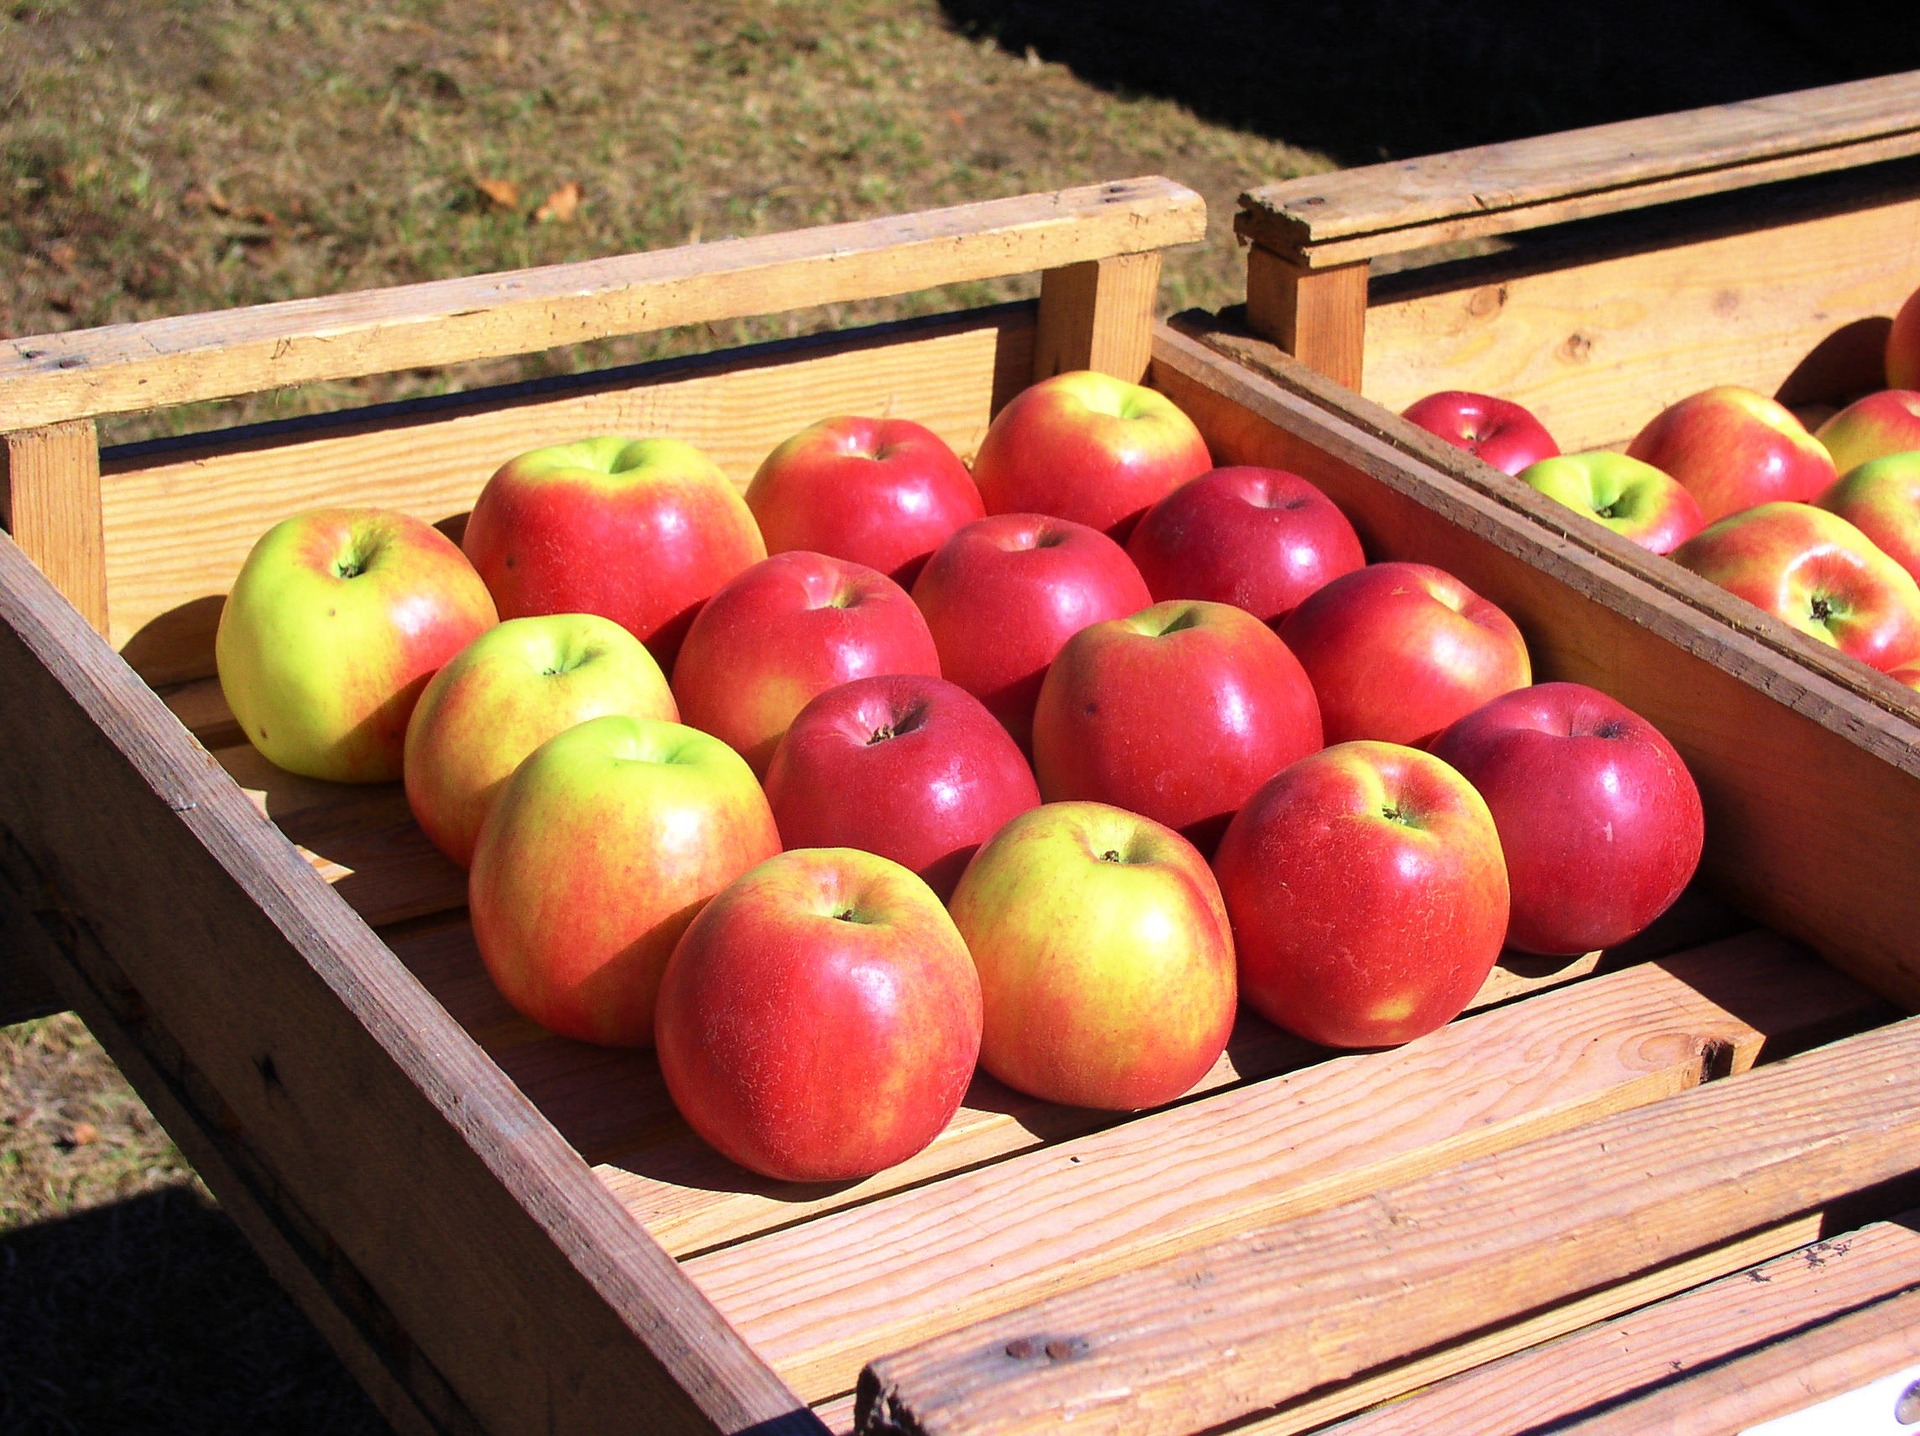
\includegraphics[max width=\linewidth, center]{external/jpg-source/apples-1642732_1920.jpg}
\end{image}%
\end{exploration}%
\footnotetext[21]{\nolinkurl{pixabay.com/photos/apples-fruit-apple-1642732/}\label{warm-cuantosVes-Manzanas-2-2-2-1-2}}%
\end{subsubsectionptx}
%
%
\typeout{************************************************}
\typeout{Subsubsección  Actividad 1}
\typeout{************************************************}
%
\clearpage
\begin{subsubsectionptx}{Subsubsección}{Actividad 1}{}{Actividad 1}{}{}{lec-cuantosGrupos-act1}
\begin{activity}{Actividad}{¿Cuántas manzanas?}{act-cuantasManzanas}%
Resuelve cada problema. Muestra cómo pensaste. Usa objetos, un dibujo o un diagrama.%
\par
%
\begin{enumerate}
\item{}Si 24 manzanas se ponen en cajas y en cada caja se ponen 8 manzanas, ¿cuántas cajas hay?%
\item{}Si 42 manzanas se ponen en cajas y en cada caja se ponen 6 manzanas, ¿cuántas cajas hay?%
\item{}Si 32 manzanas se ponen en cajas y en cada caja se ponen 4 manzanas, ¿cuántas cajas hay?%
\end{enumerate}
%
\end{activity}%
\end{subsubsectionptx}
%
%
\typeout{************************************************}
\typeout{Subsubsección  Actividad 2}
\typeout{************************************************}
%
\begin{subsubsectionptx}{Subsubsección}{Actividad 2}{}{Actividad 2}{}{}{lec-cuantosGrupos-act2}
\begin{activity}{Actividad}{Recorrido por el salón: Manzanas en cajas.}{act-recorridoSalon-manzanasEnCajas}%
%
\begin{enumerate}
\item{}Con tu compañero, ve a ver los pósteres alrededor del salón. Discute con tu compañero en qué se parecen y en qué se diferencian las ideas que se muestran en los pósteres.%
\item{}Reflexiona sobre lo que viste. Escribe una cosa en la que se parecen y una cosa en la que se diferencian las ideas que se muestran en los pósteres.%
\end{enumerate}
%
\end{activity}%
\end{subsubsectionptx}
\end{subsectionptx}
%
%
\typeout{************************************************}
\typeout{Subsección  Lección 2 -~¿Cuántos hay en cada grupo?}
\typeout{************************************************}
%
\begin{subsectionptx}{Subsección}{{\normalsize Lección 2\\[-0.05cm]}¿Cuántos hay en cada grupo?}{}{Lección 2}{}{}{lec-cuantosEnCadaGrupo}
\begin{introduction}{}%
Representemos y resolvamos más problemas.%
\end{introduction}%
%
%
\typeout{************************************************}
\typeout{Subsubsección  Calentamiento}
\typeout{************************************************}
%
\begin{subsubsectionptx}{Subsubsección}{Calentamiento}{}{Calentamiento}{}{}{lec-cuantosEnCadaGrupo-warm}
\begin{exploration}{Calentamiento}{Observa y pregúntate: Más manzanas.}{warm-observa-arbolManzanas}%
¿Qué observas?\\
 ¿Qué te preguntas?%
\begin{image}{0.15}{0.7}{0.15}{}%
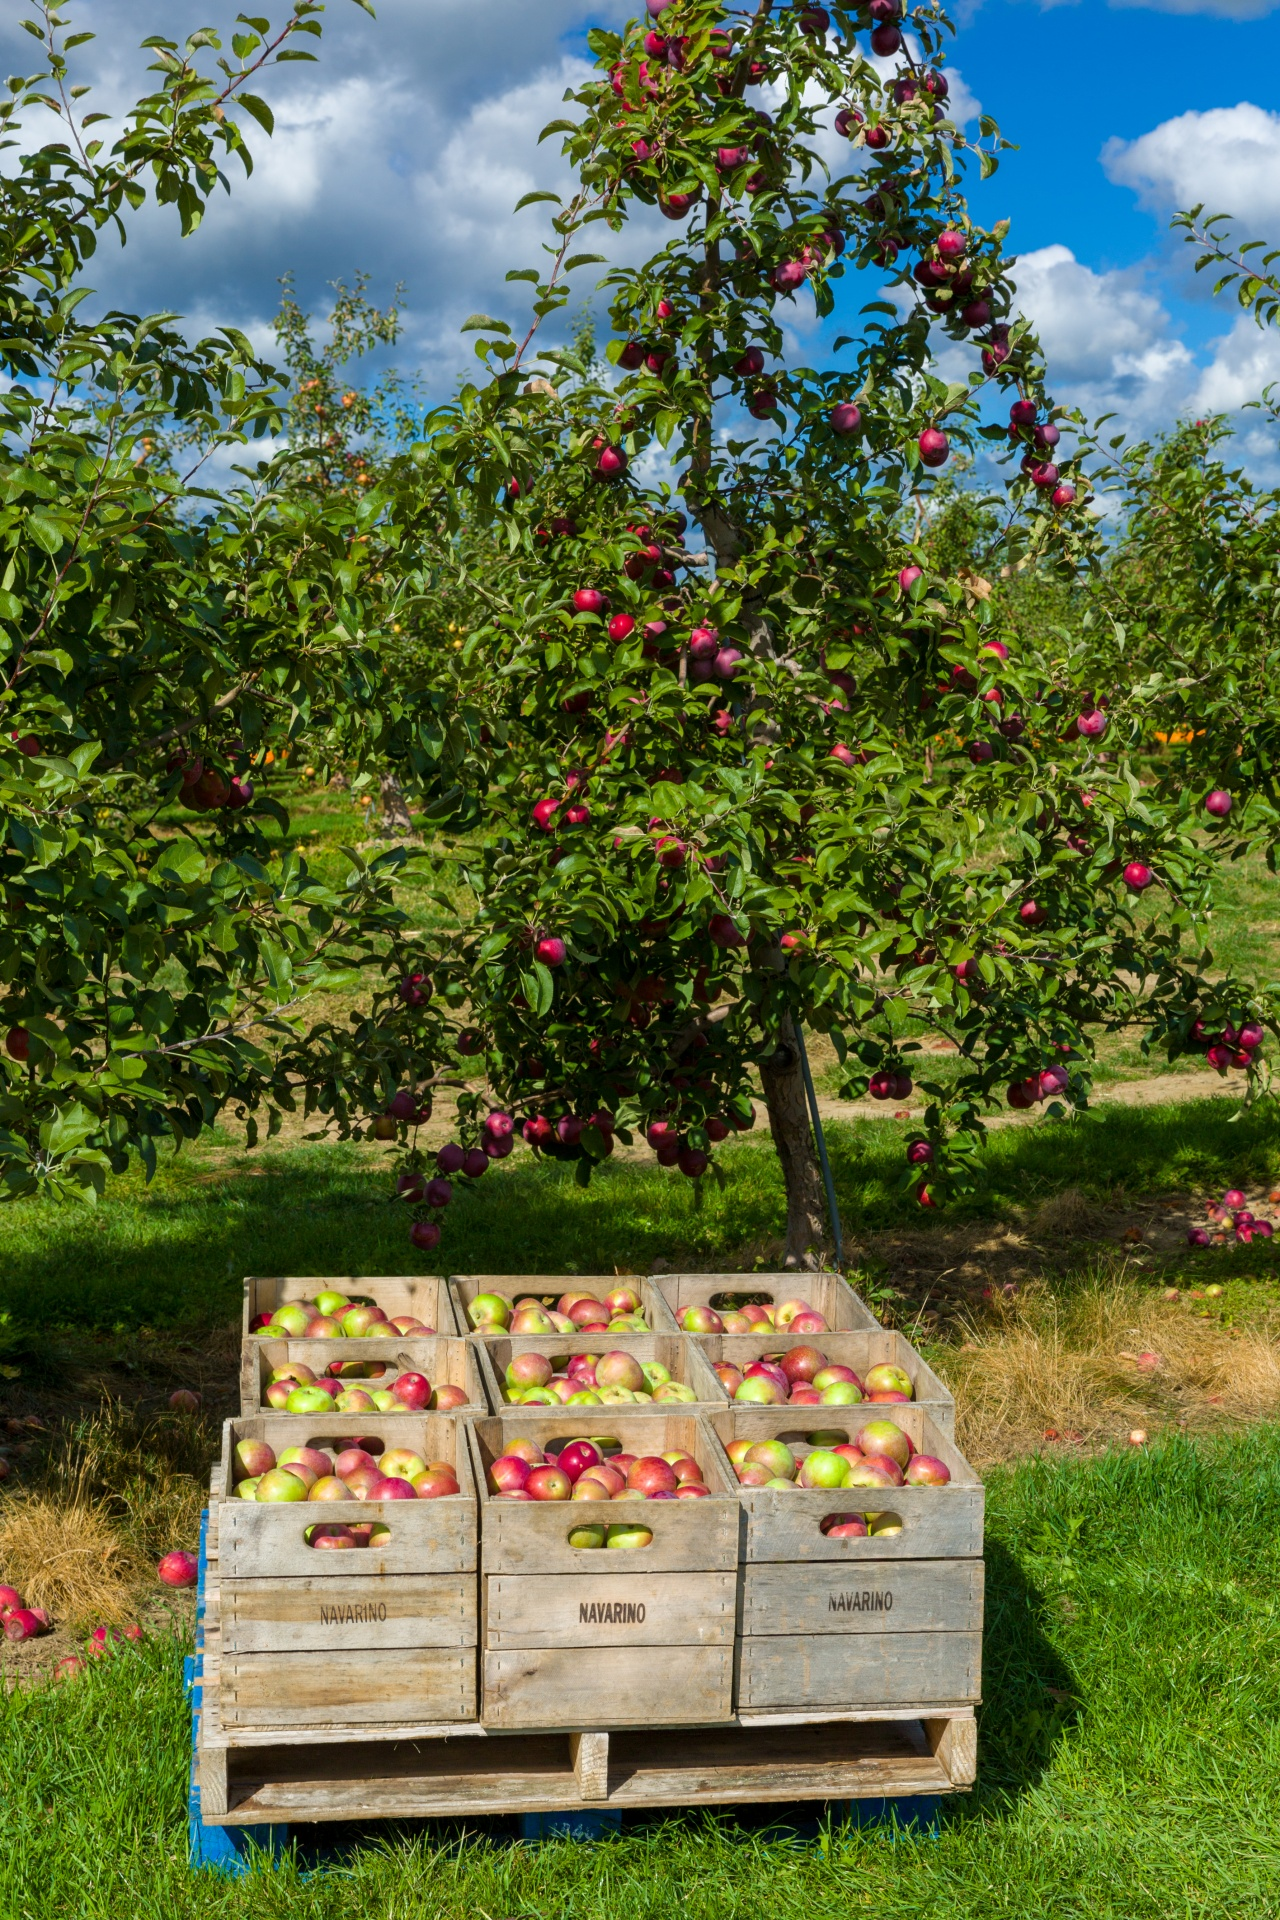
\includegraphics[max width=\linewidth, center]{external/jpg-source/3.4.A2 Warm-up.jpg}
\end{image}%
\end{exploration}%
\footnotetext[22]{\nolinkurl{www.publicdomainpictures.net/en/view-image.php?image=267667\&picture=apple-orchard}\label{warm-observa-arbolManzanas-2-2-2-1-2}}%
\end{subsubsectionptx}
%
%
\typeout{************************************************}
\typeout{Subsubsección  Actividad 1}
\typeout{************************************************}
%
\begin{subsubsectionptx}{Subsubsección}{Actividad 1}{}{Actividad 1}{}{}{lec-cuantosEnCadaGrupo-act1}
\begin{activity}{Actividad}{¿Cuántas manzanas?}{act-cuantasManzanas2}%
Resuelve cada problema. Muestra cómo pensaste. Usa objetos, un dibujo o un diagrama.%
\par
%
\begin{enumerate}
\item{}Si 20 manzanas se empacan en 4 cajas y en cada caja hay el mismo número de manzanas, ¿cuántas manzanas hay en cada caja?%
\item{}Si 36 manzanas se empacan en 6 cajas y en cada caja hay el mismo número de manzanas, ¿cuántas manzanas hay en cada caja?%
\item{}Si 45 manzanas se empacan en 9 cajas y en cada caja hay el mismo número de manzanas, ¿cuántas manzanas hay en cada caja?%
\end{enumerate}
%
\end{activity}%
\end{subsubsectionptx}
%
%
\typeout{************************************************}
\typeout{Subsubsección  Actividad 2}
\typeout{************************************************}
%
\begin{subsubsectionptx}{Subsubsección}{Actividad 2}{}{Actividad 2}{}{}{lec-cuantosEnCadaGrupo-act2}
\begin{activity}{Actividad}{Recorrido por el salón.}{act-recorridoSalon-Manzanas2}%
Con tu compañero, ve a ver los pósteres alrededor del salón. Discute con tu compañero en qué se parecen y en qué se diferencian las ideas que se muestran en los pósteres.%
\end{activity}%
\end{subsubsectionptx}
%
%
\typeout{************************************************}
\typeout{Subsubsección  Actividad 3}
\typeout{************************************************}
%
\begin{subsubsectionptx}{Subsubsección}{Actividad 3}{}{Actividad 3}{}{}{lec-cuantosEnCadaGrupo-act3}
\begin{activity}{Actividad}{Todas las manzanas.}{act-todasLasManzanas}%
\begin{sidebyside}{2}{0.05}{0.05}{0.1}%
\begin{sbspanel}{0.4}%
Si 24 manzanas se ponen en cajas y en cada caja se ponen 8 manzanas, ¿cuántas cajas hay?%
\end{sbspanel}%
\begin{sbspanel}{0.4}%
\par
Si 20 manzanas se empacan en 4 cajas y cada caja tiene el mismo número de manzanas, ¿cuántas manzanas hay en cada caja?%
\end{sbspanel}%
\end{sidebyside}%
\par
Discute con tu compañero:%
\par
%
\begin{itemize}[label=\textbullet]
\item{}¿En qué se parecen estos problemas?%
\item{}¿En qué se diferencian?%
\item{}¿En qué se parecen y en qué se diferencian las formas de representar y resolver estos problemas?%
\end{itemize}
%
\end{activity}%
\end{subsubsectionptx}
\end{subsectionptx}
%
%
\typeout{************************************************}
\typeout{Subsección  Lección 3 -~Dibujos de situaciones de división}
\typeout{************************************************}
%
\begin{subsectionptx}{Subsección}{{\normalsize Lección 3\\[-0.05cm]}Dibujos de situaciones de división}{}{Lección 3}{}{}{lec-dibujosSituacionesDivision}
\begin{introduction}{}%
Representemos situaciones de división con dibujos.%
\end{introduction}%
%
%
\typeout{************************************************}
\typeout{Subsubsección  Calentamiento}
\typeout{************************************************}
%
\begin{subsubsectionptx}{Subsubsección}{Calentamiento}{}{Calentamiento}{}{}{lec-dibujosSituacionesDivision-warm}
\begin{exploration}{Calentamiento}{Conversación numérica: Cuanto más cambien las cosas....}{warm-numTalk-cuantoMasCambien}%
Encuentra mentalmente el valor de cada expresión.%
\par
%
\begin{enumerate}[label={\Alph*.}]
\item{}\(\displaystyle 120 + 120\)%
\item{}\(\displaystyle 121 + 119\)%
\item{}\(\displaystyle 125 + 115\)%
\item{}\(\displaystyle 129 + 111\)%
\end{enumerate}
%
\end{exploration}%
\end{subsubsectionptx}
%
%
\typeout{************************************************}
\typeout{Subsubsección  Actividad 1}
\typeout{************************************************}
%
\begin{subsubsectionptx}{Subsubsección}{Actividad 1}{}{Actividad 1}{}{}{lec-dibujosSituacionesDivision-act1}
\begin{activity}{Actividad}{Grupos de estudiantes.}{act-gruposEstudiantes}%
%
\begin{enumerate}
\item{}¿Qué observaste acerca de cómo los estudiantes se organizaron en grupos de 2?%
\item{}¿Qué observaste acerca de cómo los estudiantes se organizaron en 2 grupos?%
\end{enumerate}
%
\end{activity}%
\end{subsubsectionptx}
%
%
\typeout{************************************************}
\typeout{Subsubsección  Actividad 2}
\typeout{************************************************}
%
\begin{subsubsectionptx}{Subsubsección}{Actividad 2}{}{Actividad 2}{}{}{lec-dibujosSituacionesDivision-act2}
\begin{activity}{Actividad}{Los lápices de colores de Elena.}{act-lapicesColores}%
Elena tiene 12 lápices de colores. Ella tiene 2 cajas y quiere poner el mismo número de lápices en cada caja. ¿Cuántos lápices irán en cada caja?%
\par
¿Cuál dibujo corresponde a la situación? Explica tu razonamiento.%
\begin{sidebyside}{2}{0}{0}{0}%
\begin{sbspanel}{0.5}%
A%
\par
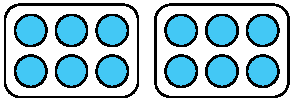
\includegraphics[max width=\linewidth, center]{external/tikz-source/tikz-file-149310.pdf}
\end{sbspanel}%
\begin{sbspanel}{0.5}%
B%
\par
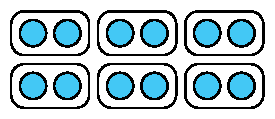
\includegraphics[max width=\linewidth, center]{external/tikz-source/tikz-file-149311.pdf}
\end{sbspanel}%
\end{sidebyside}%
\end{activity}%
\end{subsubsectionptx}
%
%
\typeout{************************************************}
\typeout{Subsubsección  Actividad 3}
\typeout{************************************************}
%
\begin{subsubsectionptx}{Subsubsección}{Actividad 3}{}{Actividad 3}{}{}{lec-dibujosSituacionesDivision-act3}
\begin{activity}{Actividad}{¿Cuál dibujo corresponde?}{act-cualDibujoCorresponde}%
Asocia cada situación con un dibujo. Prepárate para explicar tu razonamiento.%
\begin{sidebyside}{2}{0}{0}{0.05}%
\begin{sbspanel}{0.55}[center]%
%
\begin{enumerate}
\item{}Mai tiene 8 marcadores y varias cajas. Ella pone 4 marcadores en cada caja. ¿Cuántas cajas con marcadores hay?%
\item{}Kiran tiene 20 bolígrafos y varias mesas. Él pone 2 bolígrafos en cada mesa. ¿En cuántas mesas puede poner bolígrafos?%
\item{}Lin tiene 8 lápices de colores y 2 bolsas. En cada bolsa pone el mismo número de lápices de colores. ¿Cuántos lápices de colores habrá en cada bolsa?%
\item{}Priya tiene 15 crayones y varios pupitres. Ella pone 5 crayones en cada pupitre. ¿En cuántos pupitres pondrá crayones?%
\item{}Noah tiene 20 lápices y 10 cajas. Él pone el mismo número de lápices en cada caja. ¿Cuántos lápices habrá en cada caja?%
\item{}Jada tiene 15 marcadores y 3 mesas. Ella pone el mismo número de marcadores en cada mesa. ¿Cuántos marcadores habrá en cada mesa?%
\end{enumerate}
\end{sbspanel}%
\begin{sbspanel}{0.4}[center]%
A.%
\par
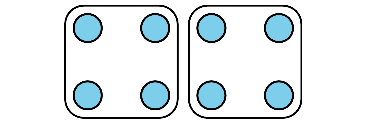
\includegraphics[max width=\linewidth, center]{external/svg-source/tikz-file-149313.pdf}
B.%
\par
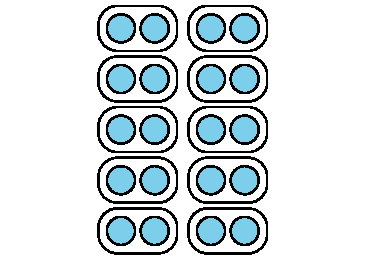
\includegraphics[max width=\linewidth, center]{external/svg-source/tikz-file-149314.pdf}
C.%
\par
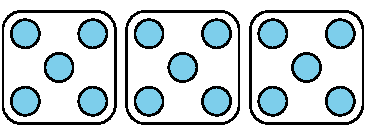
\includegraphics[max width=\linewidth, center]{external/svg-source/tikz-file-149315.pdf}
\end{sbspanel}%
\end{sidebyside}%
\end{activity}%
\end{subsubsectionptx}
\end{subsectionptx}
%
%
\typeout{************************************************}
\typeout{Subsección  Lección 4 -~Interpretemos expresiones de división}
\typeout{************************************************}
%
\begin{subsectionptx}{Subsección}{{\normalsize Lección 4\\[-0.05cm]}Interpretemos expresiones de división}{}{Lección 4}{}{}{lec-interpretarExpresionesDivision}
\begin{introduction}{}%
Démosle sentido a expresiones de división.%
\end{introduction}%
%
%
\typeout{************************************************}
\typeout{Subsubsección  Calentamiento}
\typeout{************************************************}
%
\begin{subsubsectionptx}{Subsubsección}{Calentamiento}{}{Calentamiento}{}{}{lec-interpretarExpresionesDivision-warm}
\begin{exploration}{Calentamiento}{Conversación numérica: ¿Más o menos?}{act-numTalk-masOMenos}%
Encuentra mentalmente el valor de cada expresión.%
%
\begin{enumerate}[label={\Alph*.}]
\item{}\(\displaystyle 500 - 475\)%
\item{}\(\displaystyle 504 - 475\)%
\item{}\(\displaystyle 512 - 475\)%
\item{}\(\displaystyle 512 - 449\)%
\end{enumerate}
\end{exploration}%
\end{subsubsectionptx}
%
%
\typeout{************************************************}
\typeout{Subsubsección  Actividad 1}
\typeout{************************************************}
%
\begin{subsubsectionptx}{Subsubsección}{Actividad 1}{}{Actividad 1}{}{}{lec-interpretarExpresionesDivision-act1}
\begin{activity}{Actividad}{Trompos.}{act-trompos}%
Los trompos son populares en todo el mundo. Estos son trompos de diferentes culturas.%
\begin{sidebyside}{5}{0}{0}{0}%
\begin{sbspanel}{0.2}%
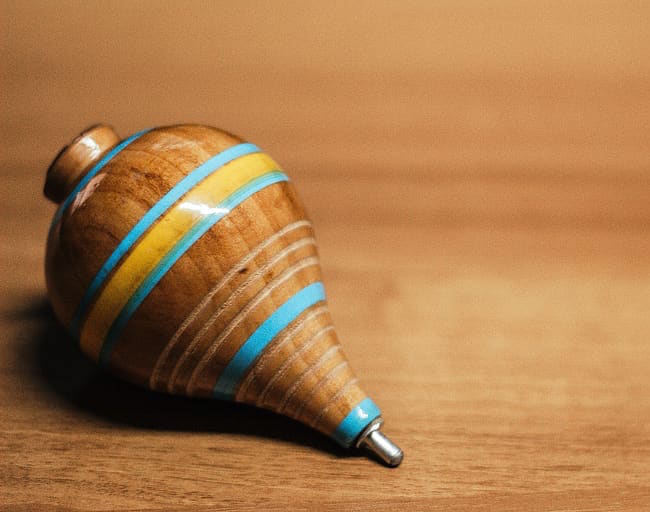
\includegraphics[max width=\linewidth, center]{external/jpg-source/V1 3.4.A.4 Mexican Trompo.jpg}
\end{sbspanel}%
\begin{sbspanel}{0.2}%
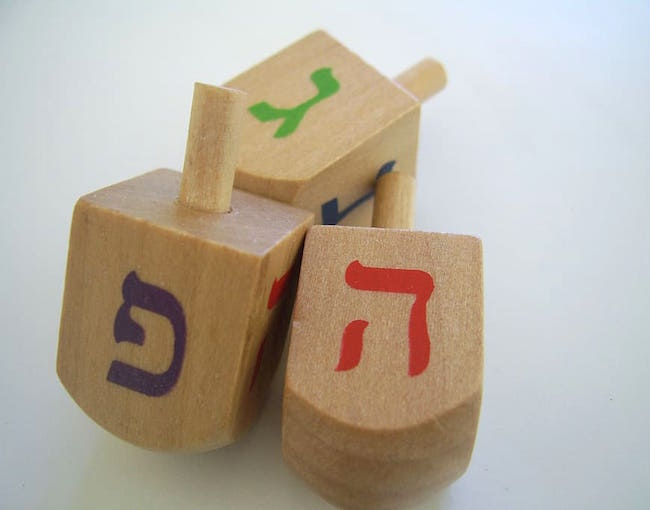
\includegraphics[max width=\linewidth, center]{external/jpg-source/V1 3.4.A.4 Dreidels.jpg}
\end{sbspanel}%
\begin{sbspanel}{0.2}%
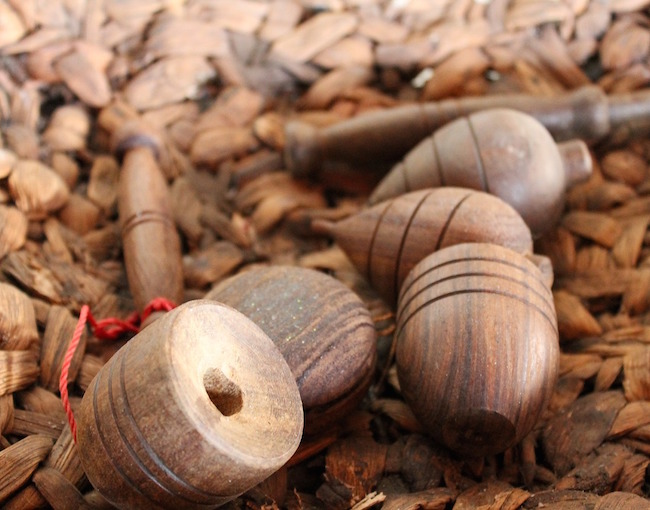
\includegraphics[max width=\linewidth, center]{external/jpg-source/V1 3.4.A.4 Indonesian Gasing.jpg}
\end{sbspanel}%
\begin{sbspanel}{0.2}%
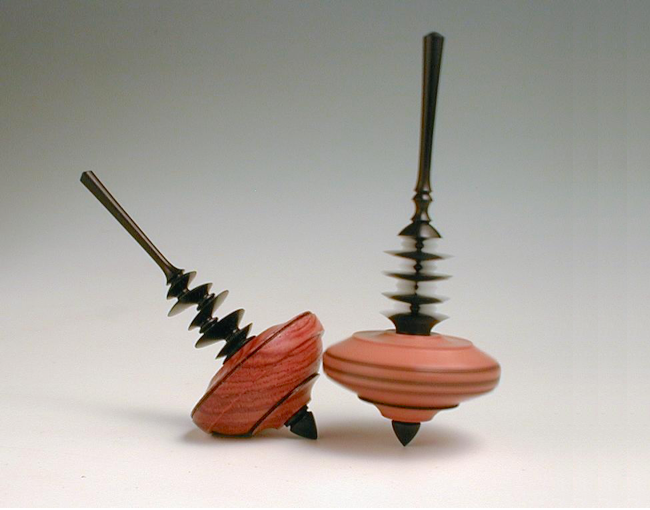
\includegraphics[max width=\linewidth, center]{external/png-source/V1 3.4.A.4 German Kreisel Copy.png}
\end{sbspanel}%
\begin{sbspanel}{0.2}%
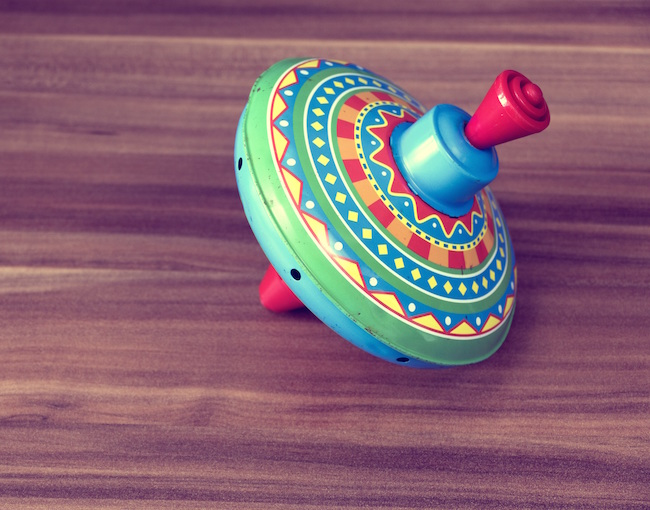
\includegraphics[max width=\linewidth, center]{external/jpg-source/V1 3.4.A.4 Colorful Top.jpg}
\end{sbspanel}%
\end{sidebyside}%
\par
Empareja cada situación sobre trompos con una expresión que pueda representarla.%
\begin{sidebyside}{2}{0.05}{0}{0.15}%
\begin{sbspanel}{0.6}%
1. Clare tiene una colección de 24 trompos de cuatro colores: negro, blanco, rojo y verde. Tiene el mismo número de trompos de cada color. ¿Cuántos trompos tiene de cada color?%
\end{sbspanel}%
\begin{sbspanel}{0.2}%
\par
A. \(24 \div 2\)%
\end{sbspanel}%
\end{sidebyside}%
\begin{sidebyside}{2}{0.05}{0}{0.15}%
\begin{sbspanel}{0.6}%
2. Priya y su amigo están decorando con pintura 24 trompos de madera. Si cada uno pinta el mismo número de trompos, ¿cuántos trompos pinta cada uno?%
\end{sbspanel}%
\begin{sbspanel}{0.2}%
\par
B. \(12 \div 2\)%
\end{sbspanel}%
\end{sidebyside}%
\begin{sidebyside}{2}{0.05}{0}{0.15}%
\begin{sbspanel}{0.6}%
3. En una tienda tienen 24 trompos de distintas partes del mundo exhibidos en 6 cajas. Cada caja contiene el mismo número de trompos. ¿Cuántos trompos hay en cada caja?%
\end{sbspanel}%
\begin{sbspanel}{0.2}%
\par
C. \(24 \div 4\)%
\end{sbspanel}%
\end{sidebyside}%
\begin{sidebyside}{2}{0.05}{0}{0.15}%
\begin{sbspanel}{0.6}%
4. Diego tiene 12 trompos que quiere regalar. Si a cada amigo le da 2 trompos, ¿cuántos amigos recibirán trompos?%
\end{sbspanel}%
\begin{sbspanel}{0.2}%
\par
D. \(12 \div 6\)%
\end{sbspanel}%
\end{sidebyside}%
\begin{sidebyside}{2}{0.05}{0}{0.15}%
\begin{sbspanel}{0.6}%
5. Seis amigos están jugando con 12 \emph{dreidels} (trompos judíos). Si cada uno juega con el mismo número de \emph{dreidels} que los demás, ¿cuántos \emph{dreidels} tiene cada uno?%
\end{sbspanel}%
\begin{sbspanel}{0.2}%
\par
E. \(24 \div 6\)%
\end{sbspanel}%
\end{sidebyside}%
\end{activity}%
\footnotetext[23]{\nolinkurl{pixabay.com/photos/wooden-spinning-top-top-mexican-3868460/}\label{act-trompos-2-2-1-2-1-2}}%
\footnotetext[24]{\nolinkurl{pixabay.com/photos/dreidels-hanukkah-spinning-tops-20347/}\label{act-trompos-2-2-2-2-1-2}}%
\footnotetext[25]{\nolinkurl{pixabay.com/photos/whirligig-traditional-folklore-wood-2316859/}\label{act-trompos-2-2-3-2-1-2}}%
\footnotetext[26]{\nolinkurl{commons.wikimedia.org/wiki/File:Spinning_Top.jpeg}\label{act-trompos-2-2-4-2-1-2}}%
\footnotetext[27]{\nolinkurl{www.pexels.com/photo/blue-and-green-spin-toy-170288/}\label{act-trompos-2-2-5-2-1-2}}%
\end{subsubsectionptx}
%
%
\typeout{************************************************}
\typeout{Subsubsección  Actividad 2}
\typeout{************************************************}
%
\begin{subsubsectionptx}{Subsubsección}{Actividad 2}{}{Actividad 2}{}{}{lec-interpretarExpresionesDivision-act2}
\begin{activity}{Actividad}{Autos en cajas.}{act-autosCajas}%
Considera estas dos situaciones.%
\begin{sidebyside}{2}{0.05}{0.05}{0.1}%
\begin{sbspanel}{0.4}%
A. Han tiene 21 autos de juguete y 3 cajas. Él pone el mismo número de autos en cada caja. ¿Cuántos autos habrá en cada caja?%
\end{sbspanel}%
\begin{sbspanel}{0.4}%
\par
B. Han tiene 21 autos de juguete y varias cajas. Él quiere poner 3 autos en cada caja. ¿Cuántas cajas necesitará?%
\end{sbspanel}%
\end{sidebyside}%
\par
¿Cuál situación está representada por la expresión \(21\div 3\)? Explica tu razonamiento.%
\end{activity}%
\end{subsubsectionptx}
%
%
\typeout{************************************************}
\typeout{Subsubsección  Actividad 3}
\typeout{************************************************}
%
\clearpage
\begin{subsubsectionptx}{Subsubsección}{Actividad 3}{}{Actividad 3}{}{}{lec-interpretarExpresionesDivision-act3}
\begin{activity}{Actividad}{Pilas de bloques.}{act-pilasBloques}%
Asocia cada situación con un dibujo y con una expresión que representan la situación. Prepárate para explicar tu razonamiento.%
%
\begin{enumerate}
\item{}Kiran usa 6 bloques para hacer pilas. Cada pila tiene 2 bloques. ¿Cuántas pilas hay?%
\item{}Han usa 6 bloques para hacer dos pilas iguales. ¿Cuántos bloques hay en cada pila?%
\item{}Jada usa 6 bloques para construir pilas que tienen 3 bloques cada una. ¿Cuántas pilas hay?%
\item{}Mai usa 6 bloques para hacer 3 pilas iguales. ¿Cuántos bloques hay en cada pila?%
\end{enumerate}
Dibujos%
\begin{sidebyside}{2}{0.05}{0.05}{0.1}%
\begin{sbspanel}{0.4}%
A%
\par
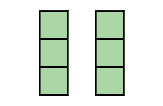
\includegraphics[max width=\linewidth, center]{external/svg-source/tikz-file-149316.pdf}
\end{sbspanel}%
\begin{sbspanel}{0.4}%
B%
\par
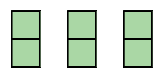
\includegraphics[max width=\linewidth, center]{external/svg-source/tikz-file-149317.pdf}
\end{sbspanel}%
\end{sidebyside}%
\par
Expresiones%
\begin{sidebyside}{2}{0.05}{0.05}{0.1}%
\begin{sbspanel}{0.4}%
C%
\begin{equation*}
6\div 2
\end{equation*}
%
\end{sbspanel}%
\begin{sbspanel}{0.4}%
\par
D%
\begin{equation*}
6\div 3
\end{equation*}
%
\end{sbspanel}%
\end{sidebyside}%
\end{activity}%
\end{subsubsectionptx}
\end{subsectionptx}
%
%
\typeout{************************************************}
\typeout{Subsección  Lección 5 -~Escribamos expresiones de división}
\typeout{************************************************}
%
\begin{subsectionptx}{Subsección}{{\normalsize Lección 5\\[-0.05cm]}Escribamos expresiones de división}{}{Lección 5}{}{}{lec-escribamosExpresionesDivision}
\begin{introduction}{}%
Escribamos expresiones de división y resolvamos problemas de “¿cuántos grupos?” y “¿cuántos hay en cada grupo?”%
\end{introduction}%
%
%
\typeout{************************************************}
\typeout{Subsubsección  Calentamiento}
\typeout{************************************************}
%
\begin{subsubsectionptx}{Subsubsección}{Calentamiento}{}{Calentamiento}{}{}{lec-escribamosExpresionesDivision-warm}
\begin{exploration}{Calentamiento}{Conversación numérica: ¿En qué se parecen?}{warm-numTalk-enQueSeParecen}%
Encuentra mentalmente el valor de cada expresión.%
\par
%
\begin{enumerate}[label={\Alph*.}]
\item{}\(\displaystyle 225 - 100\)%
\item{}\(\displaystyle 227 - 102\)%
\item{}\(\displaystyle 230 - 105\)%
\item{}\(\displaystyle 220 - 95\)%
\end{enumerate}
%
\end{exploration}%
\end{subsubsectionptx}
%
%
\typeout{************************************************}
\typeout{Subsubsección  Actividad 1}
\typeout{************************************************}
%
\begin{subsubsectionptx}{Subsubsección}{Actividad 1}{}{Actividad 1}{}{}{lec-escribamosExpresionesDivision-act1}
\begin{activity}{Actividad}{Clasificación de tarjetas: Todo sobre bichos.}{act-clasificacionDeTarjetas-todoSobreBichos}%
\begin{image}{0.3}{0.4}{0.3}{}%
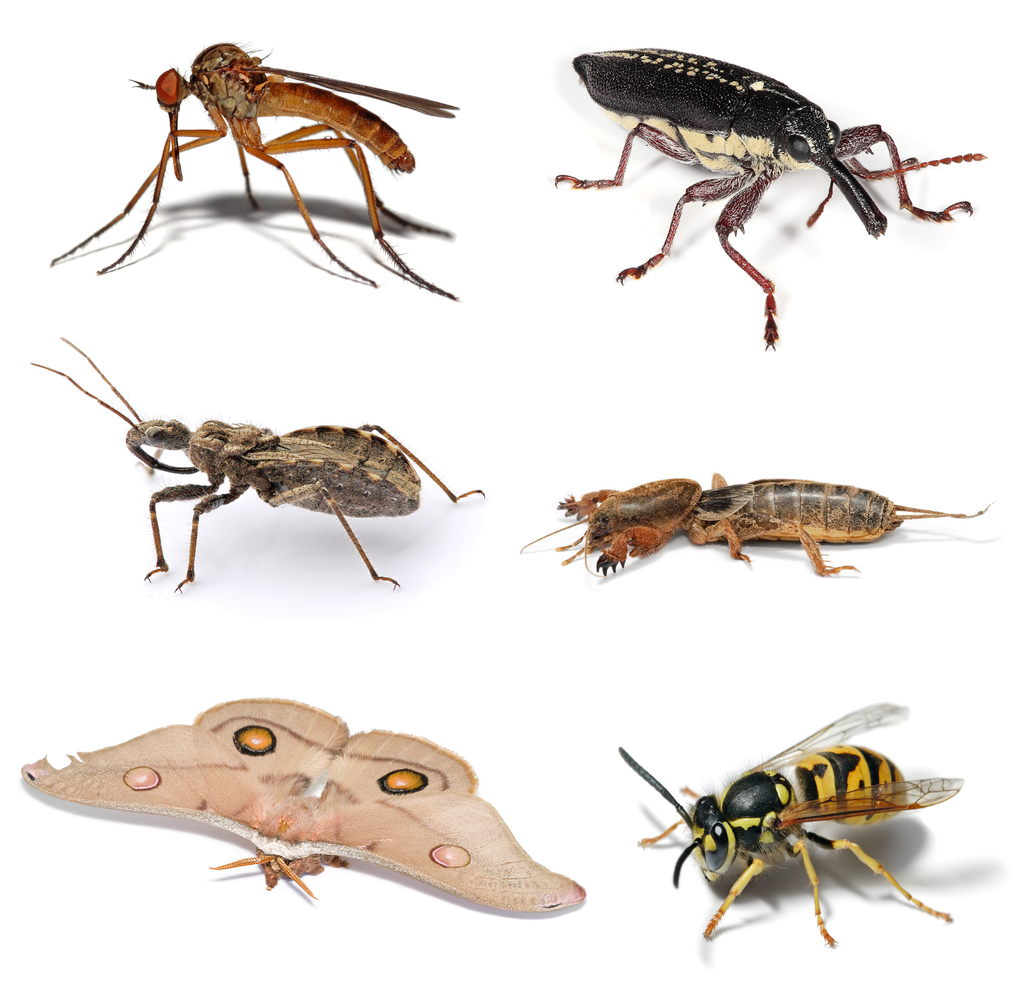
\includegraphics[max width=\linewidth, center]{external/png-source/v1 3.4.A5 Launch.png}
\end{image}%
%
\begin{enumerate}
\item{}Tu profesor te dará un grupo de tarjetas que describen situaciones. Elige dos categorías y clasifica las tarjetas en esas dos categorías. Prepárate para explicar el significado de tus categorías.%
\item{}Escribe una expresión de división para representar cada situación. Prepárate para explicar tu razonamiento.%
\end{enumerate}
\end{activity}%
\footnotetext[28]{\nolinkurl{en.wikipedia.org/wiki/File:Insect_collage.png}\label{act-clasificacionDeTarjetas-todoSobreBichos-2-1-2-1-2}}%
\end{subsubsectionptx}
%
%
\typeout{************************************************}
\typeout{Subsubsección  Actividad 2}
\typeout{************************************************}
%
\begin{subsubsectionptx}{Subsubsección}{Actividad 2}{}{Actividad 2}{}{}{lec-escribamosExpresionesDivision-act2}
\begin{activity}{Actividad}{Resolvamos un problema sobre bichos.}{act-resolvamosProblemaBichos}%
Tu profesor les va a asignar un problema.%
\par
Hagan una presentación visual que muestre cómo pensaron y que muestre su solución al problema.%
\end{activity}%
\end{subsubsectionptx}
\end{subsectionptx}
%
%
\typeout{************************************************}
\typeout{Ejercicios  Problemas de práctica de la sección A}
\typeout{************************************************}
%
\begin{exercises-subsection}{Ejercicios}{Problemas de práctica de la sección A}{}{Problemas de práctica}{}{}{gra3-uni4-secA-ProblemasPractica}
\begin{divisionexercise}{1}{(Previo a la sección).}{}{gra3-uni4-secA-ProblemasPractica-3}%
\begin{sidebyside}{2}{0}{0}{0}%
\begin{sbspanel}{0.3}%
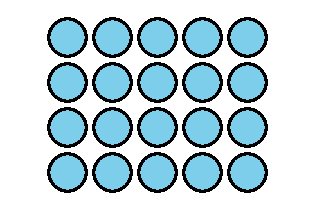
\includegraphics[max width=\linewidth, center]{external/svg-source/tikz-file-151668.pdf}
\end{sbspanel}%
\begin{sbspanel}{0.7}%
%
\begin{enumerate}[label={(\alph*)}]
\item{}Escribe una expresión de multiplicación que represente el arreglo.%
\item{}Escribe una ecuación de multiplicación que represente el arreglo.%
\end{enumerate}
%
\end{sbspanel}%
\end{sidebyside}%
\end{divisionexercise}%
\begin{divisionexercise}{2}{(Previo a la sección).}{}{gra3-uni4-secA-ProblemasPractica-4}%
Encuentra el área de cada rectángulo.%
\begin{sidebyside}{2}{0.05}{0.05}{0.1}%
\begin{sbspanel}{0.3}%
A.%
\par
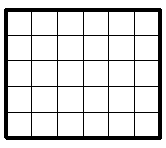
\includegraphics[max width=\linewidth, center]{external/svg-source/tikz-file-151669-scale13.pdf}
\end{sbspanel}%
\begin{sbspanel}{0.5}%
B.%
\par
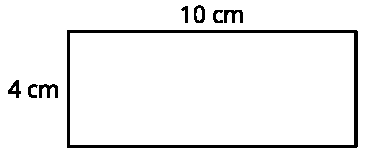
\includegraphics[max width=\linewidth, center]{external/svg-source/tikz-file-151670-scale13.pdf}
\end{sbspanel}%
\end{sidebyside}%
\end{divisionexercise}%
\begin{divisionexercise}{3}{(Previo a la sección).}{}{gra3-uni4-secA-ProblemasPractica-5}%
El área del rectángulo es 40 centímetros cuadrados.%
\begin{sidebyside}{2}{0}{0}{0}%
\begin{sbspanel}{0.5}%
Encuentra la longitud de lado desconocida del rectángulo. Explica tu razonamiento.%
\end{sbspanel}%
\begin{sbspanel}{0.5}%
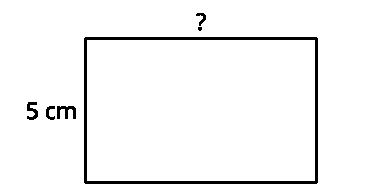
\includegraphics[max width=\linewidth, center]{external/svg-source/tikz-file-151673-scale13.pdf}
\end{sbspanel}%
\end{sidebyside}%
\end{divisionexercise}%
\begin{divisionexercise}{4}{(Previo a la sección).}{}{gra3-uni4-secA-ProblemasPractica-6}%
En cada caso, encuentra el número que hace que la ecuación sea verdadera.%
\par
%
\begin{enumerate}[label={(\alph*)}]
\item{}\(\displaystyle 8 \times 5 = \underline{\hspace{1cm}}\)%
\item{}\(\displaystyle 5 \times \underline{\hspace{1cm}} = 35\)%
\item{}\(\displaystyle \underline{\hspace{1cm}} \times 2 = 18\)%
\end{enumerate}
%
\end{divisionexercise}%
\begin{divisionexercise}{5}{(Previo a la sección).}{}{gra3-uni4-secA-ProblemasPractica-7}%
Hay 6 equipos de voleibol en el gimnasio. Cada equipo tiene 10 jugadores. ¿Cuántos jugadores de voleibol hay en total?%
\par
%
\begin{enumerate}[label={(\alph*)}]
\item{}Haz un dibujo de la situación.%
\item{}Escribe una ecuación que represente la situación. Usa un “?” para representar el valor desconocido.%
\item{}Resuelve el problema.%
\end{enumerate}
%
\end{divisionexercise}%
\begin{divisionexercise}{6}{}{}{gra3-uni4-secA-ProblemasPractica-8}%
En cada problema, usa un dibujo o un diagrama para mostrar cómo pensaste.%
\par
%
\begin{enumerate}[label={(\alph*)}]
\item{}Hay 40 manzanas empacadas en cajas. Si hay 8 manzanas en cada caja, ¿cuántas cajas hay?%
\item{}Hay 40 manzanas empacadas en cajas. Si hay 10 manzanas en cada caja, ¿cuántas cajas hay?%
\end{enumerate}
%
\end{divisionexercise}%
\begin{divisionexercise}{7}{}{}{gra3-uni4-secA-ProblemasPractica-9}%
En cada problema, usa un dibujo o un diagrama para mostrar cómo pensaste.%
%
\begin{enumerate}[label={(\alph*)}]
\item{}Hay 30 naranjas. Las empacan en 5 bolsas. Si hay la misma cantidad de naranjas en cada bolsa, ¿cuántas naranjas hay en cada bolsa?%
\item{}Hay 30 naranjas. Las empacan en 3 bolsas. Si hay la misma cantidad de naranjas en cada bolsa, ¿cuántas naranjas hay en cada bolsa?%
\end{enumerate}
\end{divisionexercise}%
\begin{divisionexercise}{8}{}{}{gra3-uni4-secA-ProblemasPractica-10}%
%
\begin{enumerate}[label={(\alph*)}]
\item{}10 personas van a cine en automóviles. En cada automóvil van dos personas. ¿Cuántos automóviles hay? Muestra cómo pensaste. Usa un dibujo o un diagrama.%
\item{}Otras 10 personas van a cine en automóviles. Van en 2 automóviles con el mismo número de personas en cada automóvil. ¿Cuántas personas hay en cada automóvil? Muestra cómo pensaste. Usa un dibujo o un diagrama.%
\item{}¿En qué se parecen las dos situaciones? ¿En qué son diferentes? ¿En qué se parecen los diagramas? ¿En qué son diferentes?%
\end{enumerate}
%
\end{divisionexercise}%
\clearpage
\begin{divisionexercise}{9}{}{}{gra3-uni4-secA-ProblemasPractica-11}%
Hay 20 pupitres en la clase. Están divididos equitativamente en 5 grupos (es decir, la misma cantidad de pupitres en cada grupo). ¿Cuántos pupitres hay en cada grupo?%
\par
%
\begin{enumerate}[label={(\alph*)}]
\item{}¿Cuál expresión representa esta situación: \(20\div 4\) o \(20\div 5\)? Explica tu razonamiento.%
\item{}Selecciona el diagrama que representa esta situación. Explica tu razonamiento.%
\begin{sidebyside}{2}{0}{0}{0}%
\begin{sbspanel}{0.07}%
A%
\end{sbspanel}%
\begin{sbspanel}{0.93}%
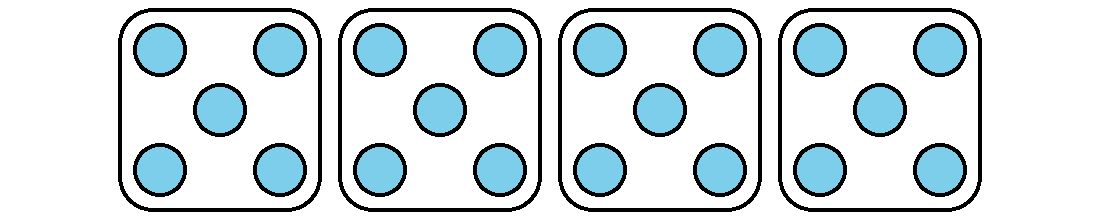
\includegraphics[max width=\linewidth, center]{external/svg-source/tikz-file-151671.pdf}
\end{sbspanel}%
\end{sidebyside}%
\begin{sidebyside}{2}{0}{0}{0}%
\begin{sbspanel}{0.07}%
B%
\end{sbspanel}%
\begin{sbspanel}{0.93}%
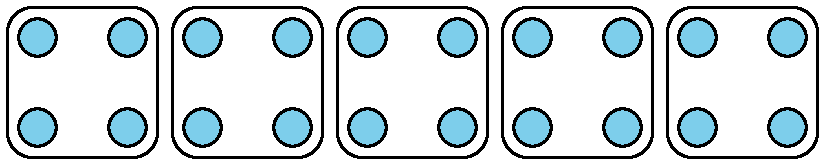
\includegraphics[max width=\linewidth, center]{external/svg-source/tikz-file-151672.pdf}
\end{sbspanel}%
\end{sidebyside}%
\end{enumerate}
%
\end{divisionexercise}%
\begin{divisionexercise}{10}{}{}{gra3-uni4-secA-ProblemasPractica-12}%
Los papás de Mai recolectaron 40 libras de duraznos y los pusieron en bolsas. Pusieron 5 libras en cada bolsa.%
\par
%
\begin{enumerate}[label={(\alph*)}]
\item{}Escribe una expresión de división que represente la situación.%
\item{}¿Cuántas bolsas de duraznos necesitaron los papás de Mai? Explica o muestra tu razonamiento.%
\end{enumerate}
%
\end{divisionexercise}%
\begin{divisionexercise}{11}{Exploración.}{}{gra3-uni4-secA-ProblemasPractica-13}%
Completa cada historia poniendo un número que tenga sentido en el espacio en blanco. Después, responde las preguntas. Dibuja un diagrama para resolver cada problema.%
\par
%
\begin{enumerate}[label={(\alph*)}]
\item{}Mai tiene \textunderscore{}\textunderscore{}\textunderscore{}\textunderscore{}\textunderscore{}\textunderscore{}\textunderscore{}\textunderscore{}\textunderscore{}\textunderscore{} calcomanías. Ella va a poner el mismo número de calcomanías en cada uno de sus 5 cuadernos. ¿Cuántas calcomanías habrá en cada cuaderno?%
\item{}Andre tiene \textunderscore{}\textunderscore{}\textunderscore{}\textunderscore{}\textunderscore{}\textunderscore{}\textunderscore{}\textunderscore{}\textunderscore{}\textunderscore{} tarjetas. Él va a organizarlas en filas de \textunderscore{}\textunderscore{}\textunderscore{}\textunderscore{}\textunderscore{}\textunderscore{}\textunderscore{}\textunderscore{}\textunderscore{}\textunderscore{} tarjetas. ¿Cuántas filas de tarjetas hará Andre?%
\end{enumerate}
%
\end{divisionexercise}%
\clearpage
\begin{divisionexercise}{12}{Exploración.}{}{gra3-uni4-secA-ProblemasPractica-14}%
Escribe una situación de división que corresponda a cada diagrama.%
\begin{sidebyside}{3}{0}{0}{0.02}%
\begin{sbspanel}{0.32}%
A%
\par
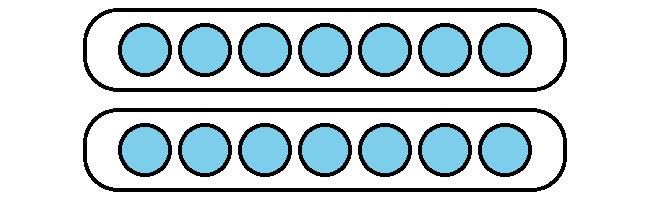
\includegraphics[max width=\linewidth, center]{external/svg-source/tikz-file-151674.pdf}
\end{sbspanel}%
\begin{sbspanel}{0.32}%
B%
\par
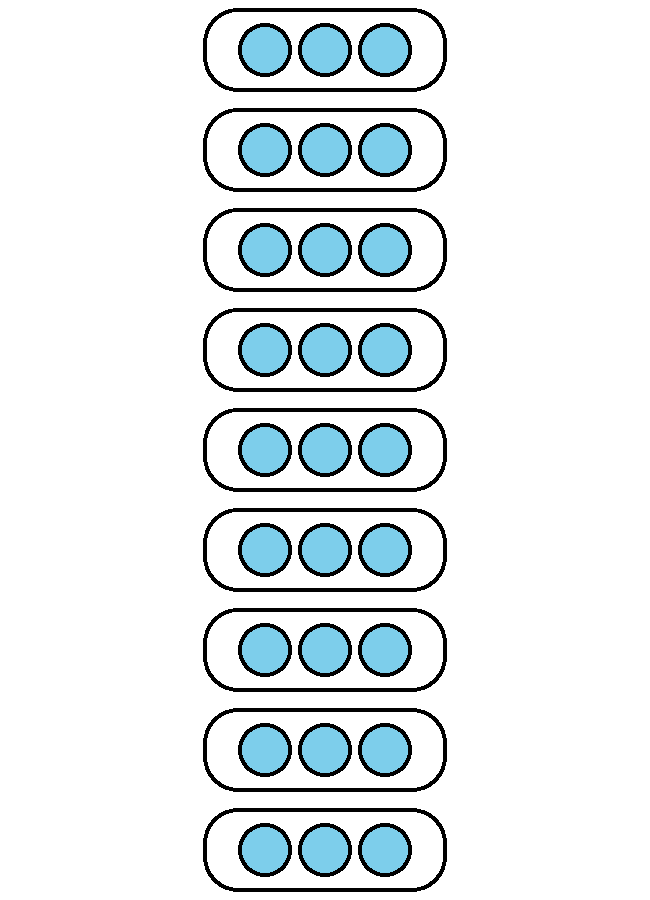
\includegraphics[max width=\linewidth, center]{external/svg-source/tikz-file-151675.pdf}
\end{sbspanel}%
\begin{sbspanel}{0.32}%
C%
\par
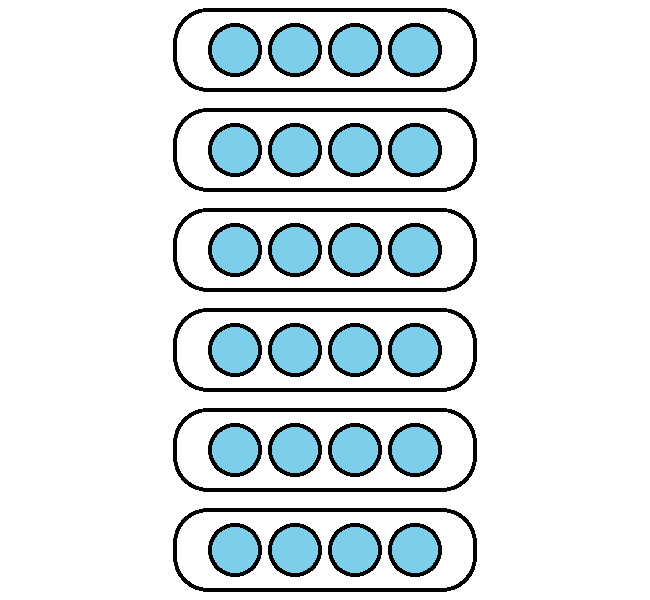
\includegraphics[max width=\linewidth, center]{external/svg-source/tikz-file-151676.pdf}
\end{sbspanel}%
\end{sidebyside}%
\end{divisionexercise}%
\end{exercises-subsection}
%
%
\typeout{************************************************}
\typeout{Referencias  Resumen de la sección}
\typeout{************************************************}
%
\begin{references-subsection}{Referencias}{Resumen de la sección}{}{Resumen sección}{}{}{gra3-uni4-secA-resumen}
En esta sección, aprendimos que la división se usa para encontrar el número de grupos o encontrar el tamaño de cada grupo cuando ponemos objetos en grupos de igual tamaño. Representamos situaciones de división con dibujos y expresiones, y resolvimos problemas de división.%
\begin{sidebyside}{2}{0.025}{0.025}{0.05}%
\begin{sbspanel}{0.45}%
``¿Cuántos grupos?''%
\end{sbspanel}%
\begin{sbspanel}{0.45}%
\par
``¿Cuántos hay en cada grupo?''%
\end{sbspanel}%
\end{sidebyside}%
\begin{sidebyside}{2}{0.025}{0.025}{0.05}%
\begin{sbspanel}{0.45}%
Han tiene 12 lápices de colores. Él quiere ponerlos en cajas. Quiere poner 2 lápices en cada caja hasta que se le acaben los lápices. ¿Cuántas cajas necesita Han?%
\end{sbspanel}%
\begin{sbspanel}{0.45}%
\par
Elena tiene 12 lápices de colores. Ella tiene 2 cajas y quiere poner el mismo número de lápices en cada caja. ¿Cuántos lápices habrá en cada caja?%
\end{sbspanel}%
\end{sidebyside}%
\begin{sidebyside}{2}{0.025}{0.025}{0.05}%
\begin{sbspanel}{0.45}%
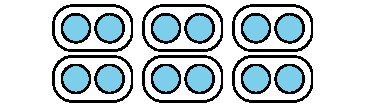
\includegraphics[max width=\linewidth, center]{external/svg-source/tikz-file-147695.pdf}
\end{sbspanel}%
\begin{sbspanel}{0.45}%
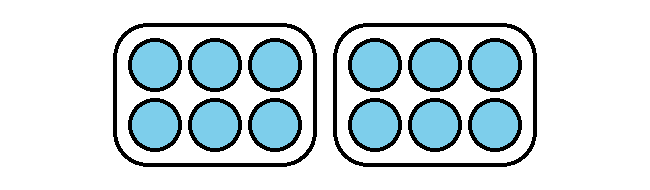
\includegraphics[max width=\linewidth, center]{external/svg-source/tikz-file-147696.pdf}
\end{sbspanel}%
\end{sidebyside}%
\begin{sidebyside}{2}{0.025}{0.025}{0.05}%
\begin{sbspanel}{0.45}%
%
\begin{equation*}
12 \div 2
\end{equation*}
%
\end{sbspanel}%
\begin{sbspanel}{0.45}%
\par
%
\begin{equation*}
12 \div 2
\end{equation*}
%
\end{sbspanel}%
\end{sidebyside}%
\end{references-subsection}
\end{sectionptx}
%
%
\typeout{************************************************}
\typeout{Sección  Sección B -~Relacionemos la multiplicación y la división}
\typeout{************************************************}
%
\begin{sectionptx}{Sección}{{\Large Sección B\\}Relacionemos la multiplicación y la división}{}{Sección B -~Relacionemos la multiplicación y la división}{}{}{gra3-uni4-secB}
%
%
\typeout{************************************************}
\typeout{Subsección  Lección 6 -~La división como un factor desconocido}
\typeout{************************************************}
%
\begin{subsectionptx}{Subsección}{{\normalsize Lección 6\\[-0.05cm]}La división como un factor desconocido}{}{Lección 6}{}{}{lec-divisionComoFactorDesconocido}
\begin{introduction}{}%
Conectemos ecuaciones de división con ecuaciones de multiplicación.%
\end{introduction}%
%
%
\typeout{************************************************}
\typeout{Subsubsección  Calentamiento}
\typeout{************************************************}
%
\begin{subsubsectionptx}{Subsubsección}{Calentamiento}{}{Calentamiento}{}{}{lec-divisionComoFactorDesconocido-warm}
\begin{exploration}{Calentamiento}{Observa y pregúntate: Números desconocidos.}{warm-observa-numerosDesconocidos}%
¿Qué observas?\\
 ¿Qué te preguntas?%
\begin{sidebyside}{2}{0}{0}{0}%
\begin{sbspanel}{0.5}%
%
\begin{equation*}
3\times {?} =12
\end{equation*}
%
\end{sbspanel}%
\begin{sbspanel}{0.5}%
\par
%
\begin{equation*}
12\div 3 ={?}
\end{equation*}
%
\end{sbspanel}%
\end{sidebyside}%
\end{exploration}%
\end{subsubsectionptx}
%
%
\typeout{************************************************}
\typeout{Subsubsección  Actividad 1}
\typeout{************************************************}
%
\begin{subsubsectionptx}{Subsubsección}{Actividad 1}{}{Actividad 1}{}{}{lec-divisionComoFactorDesconocido-act1}
\begin{activity}{Actividad}{Ecuaciones acerca de cebollas.}{act-ecuacionesCebollas}%
\begin{image}{0.15}{0.7}{0.15}{}%
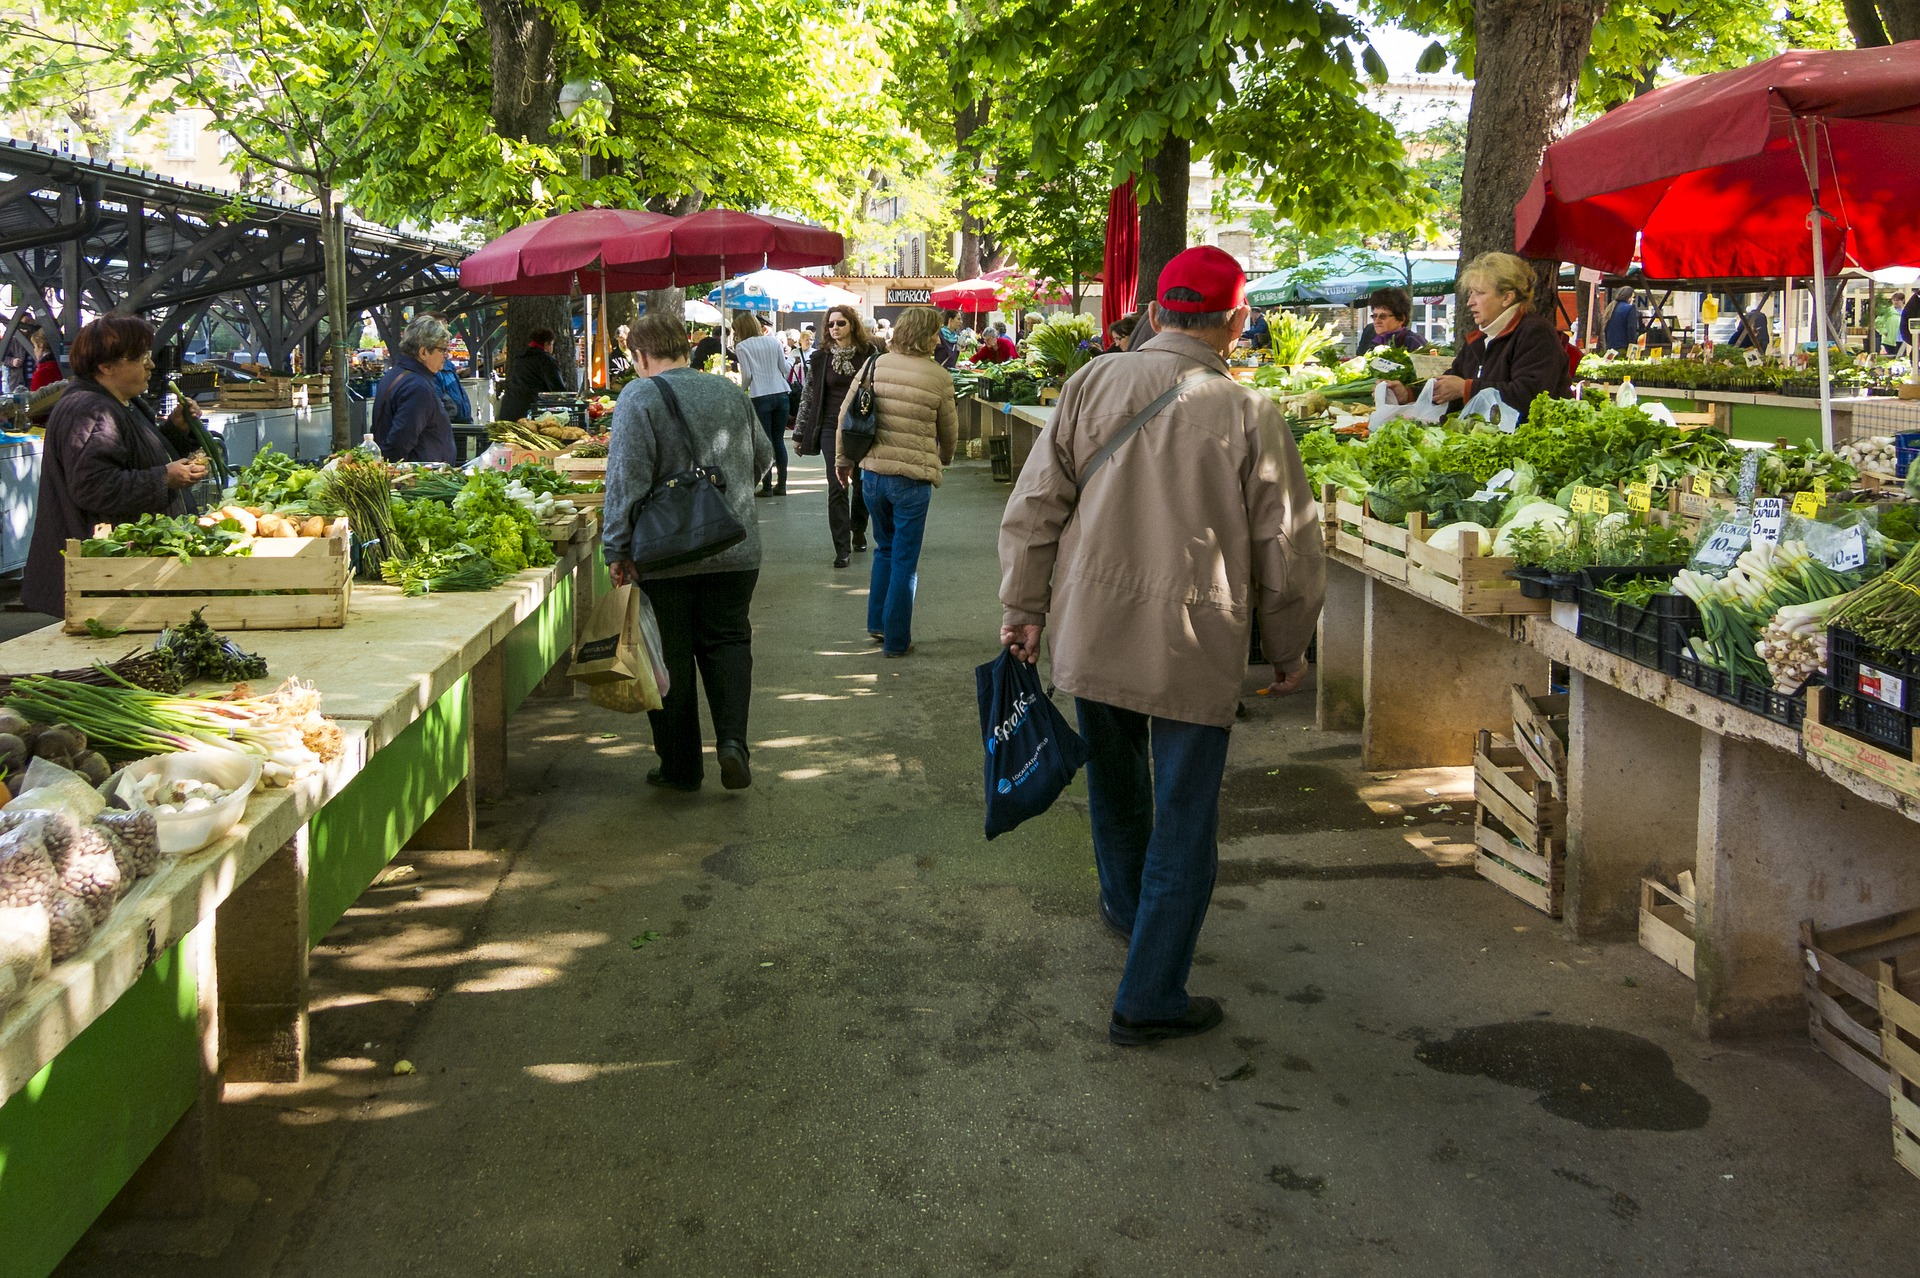
\includegraphics[width=0.7\linewidth, max width=\linewidth, center]{external/jpg-source/3.4.B6 Act 1 Launch.jpg}
\end{image}%
Un agricultor tiene 14 cebollas y 2 bolsas. Pone el mismo número de cebollas en cada bolsa.%
\par
Lin dice que la situación debe representarse con la ecuación:%
\begin{equation*}
2 \times \boxed{\phantom{3}} = 14
\end{equation*}
%
\par
Mai dice que la situación debe representarse con la ecuación:%
\begin{equation*}
14 \div 2 = \boxed{\phantom{3}}
\end{equation*}
%
\par
¿Con qué ecuación estás de acuerdo? Prepárate para explicar tu razonamiento.%
\end{activity}%
\footnotetext[29]{\nolinkurl{pixabay.com/photos/market-vegetable-market-1558658/}\label{act-ecuacionesCebollas-2-1-2-1-2}}%
\end{subsubsectionptx}
%
%
\typeout{************************************************}
\typeout{Subsubsección  Actividad 2}
\typeout{************************************************}
%
\begin{subsubsectionptx}{Subsubsección}{Actividad 2}{}{Actividad 2}{}{}{lec-divisionComoFactorDesconocido-act2}
\begin{activity}{Actividad}{En el mercado agrícola.}{act-enElMercadoAgricola}%
Completa cada fila. Prepárate para explicar tu razonamiento.%
\begin{image}{0}{1}{0}{}%
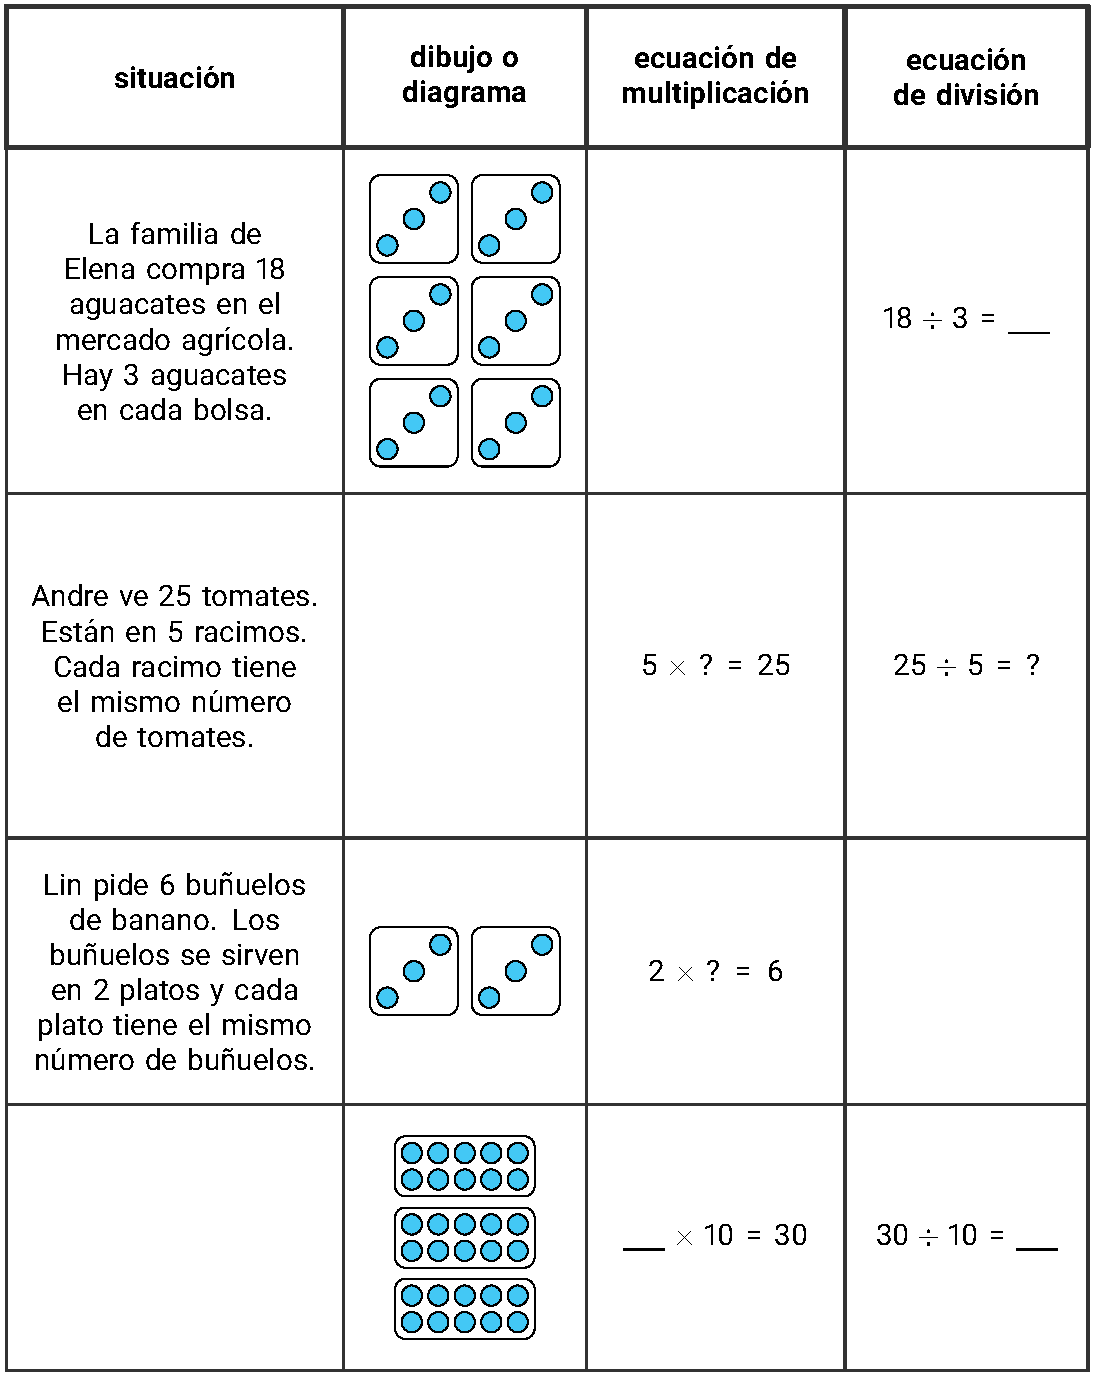
\includegraphics[max width=\linewidth, center]{external/tikz-source/enElMercadoAgricola-tab.pdf}
\end{image}%
\end{activity}%
\end{subsubsectionptx}
\end{subsectionptx}
%
%
\typeout{************************************************}
\typeout{Subsección  Lección 7 -~Relacionemos multiplicación y división}
\typeout{************************************************}
%
\begin{subsectionptx}{Subsección}{{\normalsize Lección 7\\[-0.05cm]}Relacionemos multiplicación y división}{}{Lección 7}{}{}{lec-relacionarMultiplicacionYDivision}
\begin{introduction}{}%
Hagamos más conexiones entre la multiplicación y la división.%
\end{introduction}%
%
%
\typeout{************************************************}
\typeout{Subsubsección  Calentamiento}
\typeout{************************************************}
%
\begin{subsubsectionptx}{Subsubsección}{Calentamiento}{}{Calentamiento}{}{}{lec-relacionarMultiplicacionYDivision-warm}
\begin{exploration}{Calentamiento}{Cuántos ves: Decenas.}{warm-cuantosVes-decenas}%
¿Cuántos ves?\\
 ¿Cómo lo sabes?, ¿qué ves?%
\begin{image}{0}{1}{0}{}%
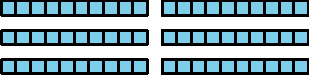
\includegraphics[max width=\linewidth, center]{external/svg-source/tikz-file-147480-scale13.pdf}
\end{image}%
\end{exploration}%
\end{subsubsectionptx}
%
%
\typeout{************************************************}
\typeout{Subsubsección  Actividad 1}
\typeout{************************************************}
%
\begin{subsubsectionptx}{Subsubsección}{Actividad 1}{}{Actividad 1}{}{}{lec-relacionarMultiplicacionYDivision-act1}
\begin{activity}{Actividad}{Mesa redonda de división.}{act-mesaRedondaDeDivision}%
Tu profesor te dará una hoja de papel con 4 recuadros. La actividad tiene 4 rondas. En cada ronda trabajarás en una hoja distinta y tu profesor te pedirá que dibujes o escribas algo en uno de los recuadros.%
\par
Después de trabajar en cada recuadro, haz una pausa y espera a que el profesor te dé las instrucciones de la siguiente ronda.%
%
\begin{enumerate}
\item{}En el recuadro 1 de tu hoja, haz un dibujo de grupos iguales.%
\item{}Observa el dibujo que tu compañero dibujó en la hoja que acabaste de recibir. En el recuadro 2, escribe una descripción de una situación de división que corresponda a ese dibujo.%
\item{}Observa los recuadros 1 y 2 de la hoja que acabaste de recibir. En el recuadro 3, escribe una ecuación de multiplicación que corresponda al dibujo y a la situación de división de esa hoja. Usa un símbolo para representar la cantidad desconocida.%
\item{}Observa los recuadros 1, 2 y 3 de la hoja que acabaste de recibir. En el recuadro 4, escribe una ecuación de división que corresponda al dibujo, a la situación de división y a la ecuación de multiplicación. Usa un símbolo para representar la cantidad desconocida.%
\end{enumerate}
\begin{image}{0.2}{0.6}{0.2}{}%
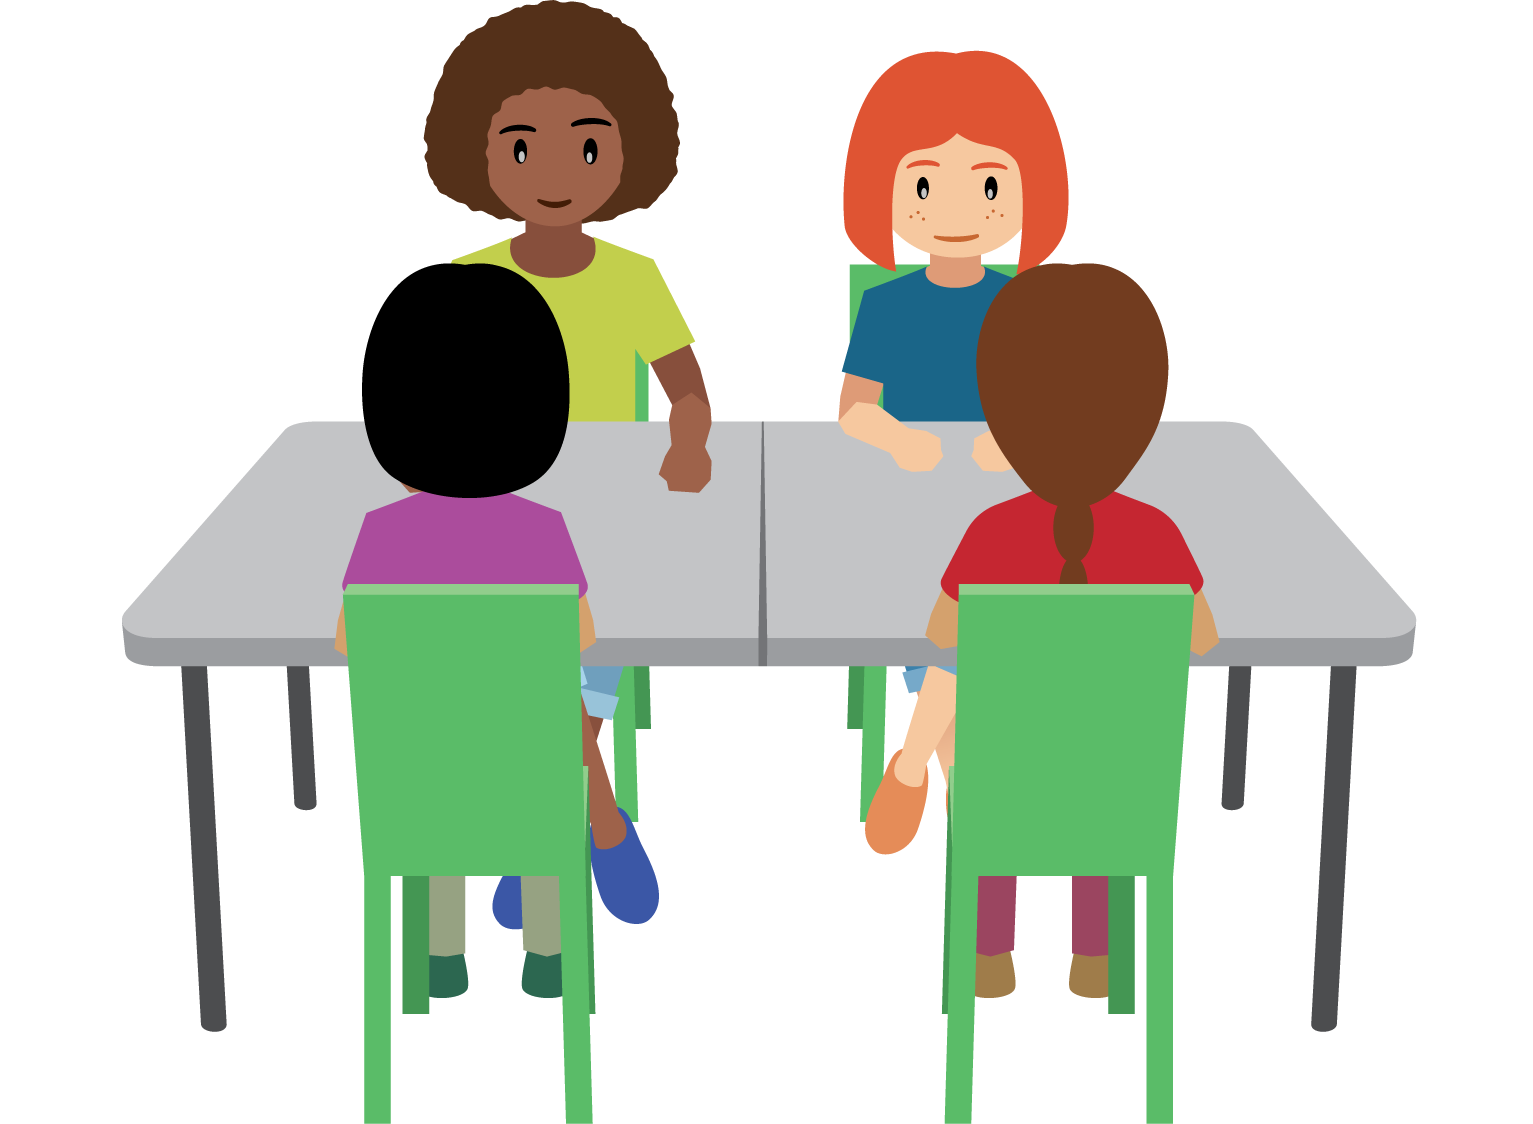
\includegraphics[max width=\linewidth, center]{external/png-source/CS 3.4 Lesson 7 Activity 1.png}
\end{image}%
\end{activity}%
\end{subsubsectionptx}
%
%
\typeout{************************************************}
\typeout{Subsubsección  Actividad 2}
\typeout{************************************************}
%
\begin{subsubsectionptx}{Subsubsección}{Actividad 2}{}{Actividad 2}{}{}{lec-relacionarMultiplicacionYDivision-act2}
\begin{activity}{Actividad}{Grupos de útiles escolares.}{act-gruposUtilesEscolares}%
En cada situación:%
\par
(a) Escribe una ecuación que represente la situación. Usa un símbolo para representar la cantidad desconocida.%
\par
(b) Resuelve el problema y encuentra el número desconocido de la ecuación. Prepárate para explicar tu razonamiento.%
\par
Situaciones:%
%
\begin{enumerate}
\item{}Kiran tenía 32 clips y los repartió entre varios estudiantes. Le dio 4 clips a cada uno. ¿Cuántos estudiantes recibieron clips?%
\item{}Hay 28 libros distribuidos en 4 pilas. Si cada pila tiene la misma cantidad de libros, ¿cuántos libros hay en cada pila?%
\item{}Hay 6 cajas. En cada caja hay 8 borradores. ¿Cuántos borradores hay en total?%
\item{}Lin tenía 36 notas adhesivas y varios cuadernos. Ella puso 6 notas adhesivas en cada cuaderno. ¿En cuántos cuadernos puso notas adhesivas?%
\end{enumerate}
\end{activity}%
\end{subsubsectionptx}
\end{subsectionptx}
%
%
\typeout{************************************************}
\typeout{Subsección  Lección 8 -~Relacionemos cocientes con productos conocidos}
\typeout{************************************************}
%
\begin{subsectionptx}{Subsección}{{\normalsize Lección 8\\[-0.05cm]}Relacionemos cocientes con productos conocidos}{}{Lección 8}{}{}{lec-relCocientesProductos}
\begin{introduction}{}%
Consideremos los productos y cocientes que nos sabemos de inmediato o que podemos encontrar rápidamente.%
\end{introduction}%
%
%
\typeout{************************************************}
\typeout{Subsubsección  Calentamiento}
\typeout{************************************************}
%
\begin{subsubsectionptx}{Subsubsección}{Calentamiento}{}{Calentamiento}{}{}{lec-relCocientesProductos-warm}
\begin{exploration}{Calentamiento}{Conversación numérica: Multiplicación y división.}{warm-numTalk-multiplicacionYDivision}%
Encuentra mentalmente el valor de cada expresión.%
%
\begin{enumerate}[label={\Alph*.}]
\item{}\(\displaystyle 4\times 10\)%
\item{}\(\displaystyle 40\div 4\)%
\item{}\(\displaystyle 40\div 10\)%
\item{}\(\displaystyle 60\div 6\)%
\end{enumerate}
\end{exploration}%
\end{subsubsectionptx}
%
%
\typeout{************************************************}
\typeout{Subsubsección  Actividad 1}
\typeout{************************************************}
%
\begin{subsubsectionptx}{Subsubsección}{Actividad 1}{}{Actividad 1}{}{}{lec-relCocientesProductos-act1}
\begin{activity}{Actividad}{Clasificación de tarjetas: Multiplicación.}{act-clasificacionDeTarjetas-multiplicacion}%
Pregúntale a tu compañero hechos de multiplicación. Clasifícalos en una de estas columnas:%
\begin{image}{0}{1}{0}{}%
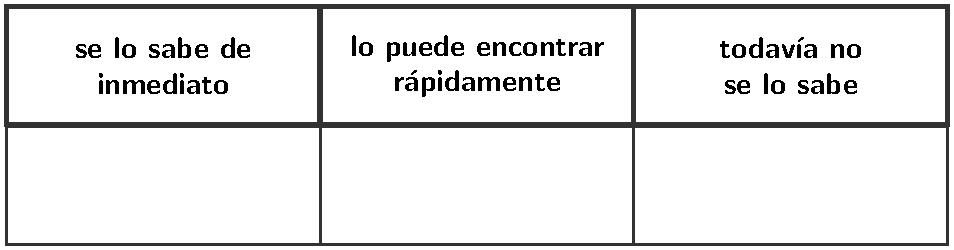
\includegraphics[max width=\linewidth, center]{external/tikz-source/clasificacionTarjetas-mult.pdf}
\end{image}%
Anota cinco expresiones de multiplicación que vas a practicar.%
\end{activity}%
\end{subsubsectionptx}
%
%
\typeout{************************************************}
\typeout{Subsubsección  Actividad 2}
\typeout{************************************************}
%
\clearpage
\begin{subsubsectionptx}{Subsubsección}{Actividad 2}{}{Actividad 2}{}{}{lec-relCocientesProductos-act2}
\begin{activity}{Actividad}{Si sé que \textellipsis{}, entonces sé que \textellipsis{}.}{act-siSeQueEntoncesSeQue}%
Si sé que \(4 \times 5 = 20\), entonces sé que \fillintext{10}.%
%
\begin{enumerate}
\item{}Coloquen las tarjetas de hechos de multiplicación en un montón, boca abajo.%
\item{}Por turnos, tomen una tarjeta de hechos de multiplicación.%
\item{}Usen el hecho de multiplicación de la tarjeta para escribir una ecuación de multiplicación en la columna “Si sé que \textellipsis{}”%
\item{}Después, en la columna “Entonces sé que   \textellipsis{}”, anoten las ecuaciones de división relacionadas.%
\end{enumerate}
\begin{image}{0}{1}{0}{}%
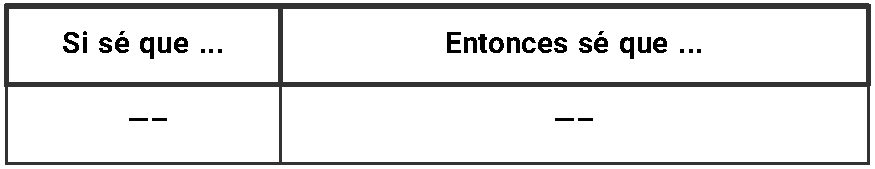
\includegraphics[max width=\linewidth, center]{external/tikz-source/siSeQueEntoncesSeQue-tab.pdf}
\end{image}%
\end{activity}%
\end{subsubsectionptx}
\end{subsectionptx}
%
%
\typeout{************************************************}
\typeout{Subsección  Lección 9 -~Patrones en la tabla de multiplicar}
\typeout{************************************************}
%
\begin{subsectionptx}{Subsección}{{\normalsize Lección 9\\[-0.05cm]}Patrones en la tabla de multiplicar}{}{Lección 9}{}{}{lec-patronesTablaMultiplicar}
\begin{introduction}{}%
Encontremos patrones en la tabla de multiplicar y usémoslos para multiplicar.%
\end{introduction}%
%
%
\typeout{************************************************}
\typeout{Subsubsección  Calentamiento}
\typeout{************************************************}
%
\begin{subsubsectionptx}{Subsubsección}{Calentamiento}{}{Calentamiento}{}{}{lec-patronesTablaMultiplicar-warm}
\begin{exploration}{Calentamiento}{Observa y pregúntate: Tabla de multiplicar.}{warm-observa-tablaMultiplicar}%
¿Qué observas?\\
 ¿Qué te preguntas?%
\begin{image}{0}{1}{0}{}%
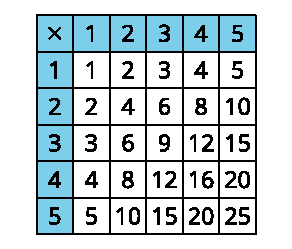
\includegraphics[max width=\linewidth, center]{external/svg-source/tikz-file-152968-scale13.pdf}
\end{image}%
\end{exploration}%
\end{subsubsectionptx}
%
%
\typeout{************************************************}
\typeout{Subsubsección  Actividad 1}
\typeout{************************************************}
%
\begin{subsubsectionptx}{Subsubsección}{Actividad 1}{}{Actividad 1}{}{}{lec-patronesTablaMultiplicar-act1}
\begin{activity}{Actividad}{Productos en la tabla.}{act-productosTablaMultiplicar}%
Esta es una tabla de multiplicar que no se ha terminado de completar.%
\begin{image}{0}{1}{0}{}%
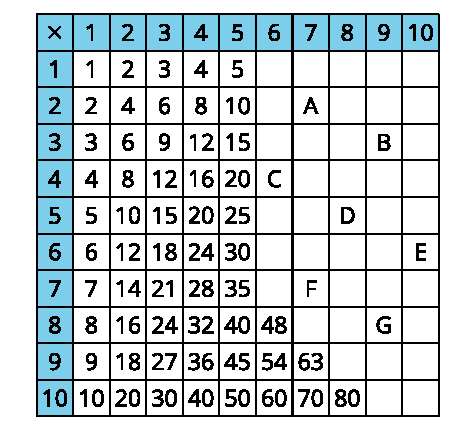
\includegraphics[max width=\linewidth, center]{external/svg-source/tikz-file-152978-scale13.pdf}
\end{image}%
%
\begin{enumerate}
\item{}Usa los productos que ya aparecen en la tabla para ayudarte a encontrar los números que deberían ir en las casillas donde están las letras de la A a la G. Prepárate para explicar tu razonamiento.%
\item{}Encuentra los números que deberían ir en otras tres casillas vacías de la tabla. Encuentra alguno que tenga:%
%
\begin{enumerate}
\item{}7 como un factor%
\item{}9 como un factor%
\item{}10 como un factor%
\end{enumerate}
Prepárate para explicar tu razonamiento.%
\end{enumerate}
\end{activity}%
\end{subsubsectionptx}
%
%
\typeout{************************************************}
\typeout{Subsubsección  Actividad 2}
\typeout{************************************************}
%
\begin{subsubsectionptx}{Subsubsección}{Actividad 2}{}{Actividad 2}{}{}{lec-patronesTablaMultiplicar-act2}
\begin{activity}{Actividad}{Si sé que \textellipsis{}, entonces sé que \textellipsis{}: Multiplicación.}{act-siSeQueEntoncesSeQueMult}%
%
\begin{enumerate}
\item{}En cada fila, escribe al menos dos hechos de multiplicación que puedes descifrar porque conoces el hecho de multiplicación dado en la columna de la izquierda. Prepárate para compartir tu razonamiento.%
\begin{image}{0}{1}{0}{}%
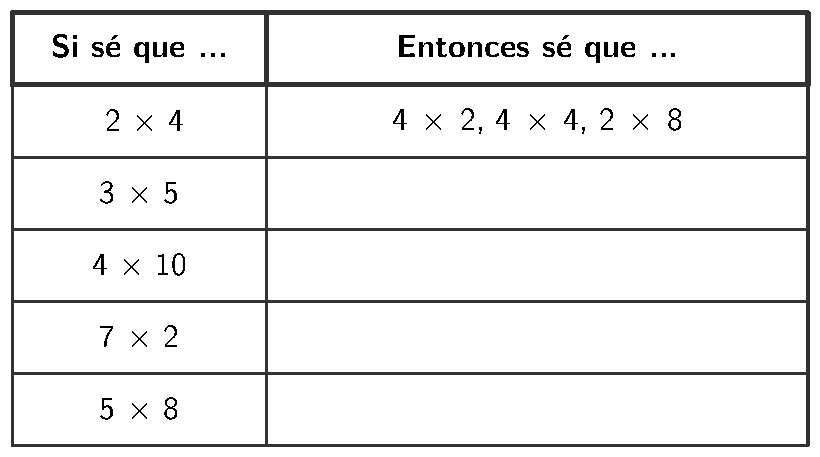
\includegraphics[max width=\linewidth, center]{external/tikz-source/siSeQueEntoncesSeQueMult-tab.pdf}
\end{image}%
\item{}Si te queda tiempo, completa el resto de la tabla de multiplicar de la actividad anterior. Usa los hechos de multiplicación que conoces para encontrar aquellos que no conoces.%
\end{enumerate}
\end{activity}%
\end{subsubsectionptx}
\end{subsectionptx}
%
%
\typeout{************************************************}
\typeout{Subsección  Lección 10 -~Exploremos estrategias de multiplicación con rectángulos}
\typeout{************************************************}
%
\begin{subsectionptx}{Subsección}{{\normalsize Lección 10\\[-0.05cm]}Exploremos estrategias de multiplicación con\\rectángulos}{}{Lección 10}{}{}{lec-estrategiasMultConRectangulos}
\begin{introduction}{}%
Usemos rectángulos para explorar estrategias de multiplicación.%
\end{introduction}%
%
%
\typeout{************************************************}
\typeout{Subsubsección  Calentamiento}
\typeout{************************************************}
%
\begin{subsubsectionptx}{Subsubsección}{Calentamiento}{}{Calentamiento}{}{}{lec-estrategiasMultConRectangulos-warm}
\begin{exploration}{Calentamiento}{Cuántos ves: Cuadrados.}{warm-cuantosVes-cuadrados}%
¿Cuántos ves?\\
 ¿Cómo lo sabes?, ¿qué ves?%
\begin{sidebyside}{3}{0}{0}{0.05}%
\begin{sbspanel}{0.3}%
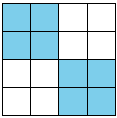
\includegraphics[max width=\linewidth, center]{external/svg-source/tikz-file-147481.pdf}
\end{sbspanel}%
\begin{sbspanel}{0.3}%
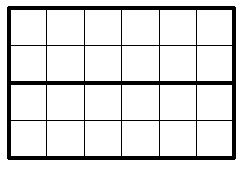
\includegraphics[max width=\linewidth, center]{external/svg-source/tikz-file-141805.pdf}
\end{sbspanel}%
\begin{sbspanel}{0.3}%
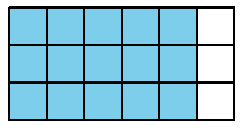
\includegraphics[max width=\linewidth, center]{external/svg-source/tikz-file-147478.pdf}
\end{sbspanel}%
\end{sidebyside}%
\end{exploration}%
\end{subsubsectionptx}
%
%
\typeout{************************************************}
\typeout{Subsubsección  Actividad 1}
\typeout{************************************************}
%
\begin{subsubsectionptx}{Subsubsección}{Actividad 1}{}{Actividad 1}{}{}{lec-estrategiasMultConRectangulos-act1}
\begin{activity}{Actividad}{De diagramas a expresiones.}{act-deDiagramasAExpresiones}%
\begin{sidebyside}{2}{0.025}{0.025}{0.05}%
\begin{sbspanel}{0.4}%
Andre y Elena están hallando el área de este rectángulo.%
\end{sbspanel}%
\begin{sbspanel}{0.5}%
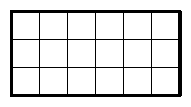
\includegraphics[max width=\linewidth, center]{external/svg-source/tikz-file-153043.pdf}
\end{sbspanel}%
\end{sidebyside}%
\begin{sidebyside}{3}{0}{0}{0.065}%
\begin{sbspanel}{0.27}%
Andre escribe \(6\times 3\).%
\end{sbspanel}%
\begin{sbspanel}{0.35}%
Él marca el rectángulo así:%
\par
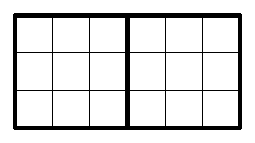
\includegraphics[max width=\linewidth, center]{external/svg-source/tikz-file-153044.pdf}
\end{sbspanel}%
\begin{sbspanel}{0.25}%
Después, Andre escribe:%
\par
\(2 \times (3 \times 3)\)\\
 \(2 \times 9 = 18\)%
\end{sbspanel}%
\end{sidebyside}%
\begin{sidebyside}{3}{0}{0}{0.065}%
\begin{sbspanel}{0.27}%
Elena escribe \(3\times 6\).%
\end{sbspanel}%
\begin{sbspanel}{0.35}%
Ella marca el rectángulo así:%
\par
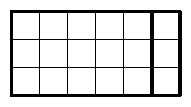
\includegraphics[max width=\linewidth, center]{external/svg-source/tikz-file-153045.pdf}
\end{sbspanel}%
\begin{sbspanel}{0.25}%
Después, Elena escribe:%
\par
\(3 \times (5 + 1)\)\\
 \((3 \times 5) + (3 \times 1)\)\\
 \(15+3\)\\
 \(18\)%
\end{sbspanel}%
\end{sidebyside}%
%
\begin{enumerate}
\item{}Discute con un compañero:%
%
\begin{enumerate}
\item{}¿En qué se parecen las estrategias de Andre y Elena? ¿En qué son diferentes?%
\item{}¿Cómo se relacionan los números de las expresiones de Andre con su diagrama?%
\item{}¿Cómo se relacionan los números de las expresiones de Elena con su diagrama?%
\end{enumerate}
\item{}Este es otro rectángulo.%
\begin{image}{0}{1}{0}{}%
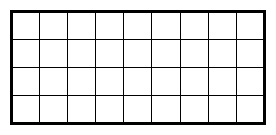
\includegraphics[max width=\linewidth, center]{external/svg-source/tikz-file-153048.pdf}
\end{image}%
Podemos encontrar su área hallando \(4 \times 9\).%
%
\begin{enumerate}
\item{}Marca o colorea el rectángulo de una manera que te ayude a encontrar su área.%
\item{}Escribe una o más expresiones que representen lo que hiciste en el diagrama y muestra cómo encontraste el área.%
\end{enumerate}
\end{enumerate}
\end{activity}%
\end{subsubsectionptx}
%
%
\typeout{************************************************}
\typeout{Subsubsección  Actividad 2}
\typeout{************************************************}
%
\begin{subsubsectionptx}{Subsubsección}{Actividad 2}{}{Actividad 2}{}{}{lec-estrategiasMultConRectangulos-act2}
\begin{activity}{Actividad}{De expresiones a diagramas.}{act-deExpresionesADiagramas}%
\begin{sidebyside}{3}{0.0166666666666667}{0.0166666666666667}{0.0333333333333333}%
\begin{sbspanel}{0.3}%
Noah%
\par
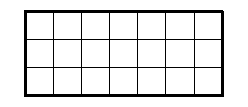
\includegraphics[max width=\linewidth, center]{external/svg-source/tikz-file-153051.pdf}
%
\begin{equation*}
(5\times 3)+(2 \times 3)
\end{equation*}
%
\end{sbspanel}%
\begin{sbspanel}{0.3}%
Priya%
\par
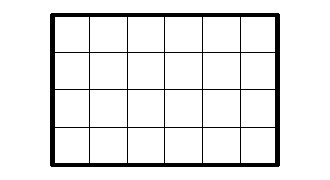
\includegraphics[max width=\linewidth, center]{external/svg-source/tikz-file-153053.pdf}
%
\begin{equation*}
2 \times (2 \times 6)
\end{equation*}
%
\end{sbspanel}%
\begin{sbspanel}{0.3}%
Tyler%
\par

\includegraphics[max width=\linewidth, center]{external/svg-source/tikz-file-153054.pdf}
%
\begin{equation*}
(5 \times 8) + (3 \times 8)
\end{equation*}
%
\end{sbspanel}%
\end{sidebyside}%
\par
En cada rectángulo:%
%
\begin{enumerate}
\item{}Escribe los dos factores que se pueden multiplicar para encontrar su área.%
\item{}Marca o colorea cada rectángulo para mostrar la manera en la que cada estudiante vio el área. Prepárate para explicar tu razonamiento.%
\end{enumerate}
\end{activity}%
\end{subsubsectionptx}
\end{subsectionptx}
%
%
\typeout{************************************************}
\typeout{Subsección  Lección 11 -~Estrategias de multiplicación para rectángulos sin cuadrícula}
\typeout{************************************************}
%
\begin{subsectionptx}{Subsección}{{\normalsize Lección 11\\[-0.05cm]}Estrategias de multiplicación para rectángulos sin\\cuadrícula}{}{Lección 11}{}{}{lec-estrategiasMultRectangulosSinCuadricula}
\begin{introduction}{}%
Usemos diferentes estrategias para encontrar el área de rectángulos sin cuadrícula.%
\end{introduction}%
%
%
\typeout{************************************************}
\typeout{Subsubsección  Calentamiento}
\typeout{************************************************}
%
\begin{subsubsectionptx}{Subsubsección}{Calentamiento}{}{Calentamiento}{}{}{gra3-uni4-secB-lec11-warm}
\begin{exploration}{Calentamiento}{Cuál es diferente: Una multiplicación representada de muchas formas.}{warm-cualDiferente-representacionesMultiplicacion}%
¿Cuál es diferente?%
\begin{sidebyside}{2}{0.05}{0.05}{0.1}%
\begin{sbspanel}{0.4}%
A%
\par
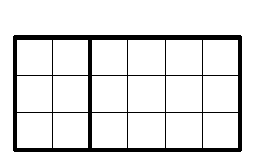
\includegraphics[max width=\linewidth, center]{external/svg-source/tikz-file-153081.pdf}
\end{sbspanel}%
\begin{sbspanel}{0.4}%
B%
\par
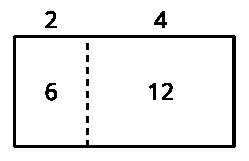
\includegraphics[max width=\linewidth, center]{external/svg-source/tikz-file-153082-scale13.pdf}
\end{sbspanel}%
\end{sidebyside}%
\begin{sidebyside}{2}{0.05}{0.05}{0.1}%
\begin{sbspanel}{0.4}%
C%
\par
%
\begin{equation*}
(3\times 2) + (3\times 4)
\end{equation*}
%
\end{sbspanel}%
\begin{sbspanel}{0.4}%
D%
\par

\includegraphics[max width=\linewidth, center]{external/svg-source/tikz-file-153083.pdf}
\end{sbspanel}%
\end{sidebyside}%
\end{exploration}%
\end{subsubsectionptx}
%
%
\typeout{************************************************}
\typeout{Subsubsección  Actividad 1}
\typeout{************************************************}
%
\clearpage
\begin{subsubsectionptx}{Subsubsección}{Actividad 1}{}{Actividad 1}{}{}{gra3-uni4-secB-lec11-act1}
\begin{activity}{Actividad}{Marca y después expresa.}{act-marcaDespuesExpresa}%
En cada caso:%
%
\begin{itemize}[label=\textbullet]
\item{}Marca o colorea cada rectángulo para mostrar una estrategia que ayude a encontrar su área.%
\item{}Escribe una o más expresiones que representen cómo encuentras el área.%
\end{itemize}
\begin{sidebyside}{3}{0}{0}{0}%
\begin{sbspanel}{0.391}%
A%
\par
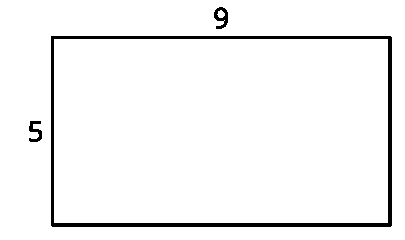
\includegraphics[max width=\linewidth, center]{external/svg-source/tikz-file-153084.pdf}
\end{sbspanel}%
\begin{sbspanel}{0.261}%
B%
\par
\includegraphics[max width=\linewidth, center]{external/svg-source/tikz-file-153085.pdf}
\end{sbspanel}%
\begin{sbspanel}{0.348}%
C%
\par
\includegraphics[max width=\linewidth, center]{external/svg-source/tikz-file-153086.pdf}
\end{sbspanel}%
\end{sidebyside}%
\end{activity}%
\end{subsubsectionptx}
%
%
\typeout{************************************************}
\typeout{Subsubsección  Actividad 2}
\typeout{************************************************}
%
\begin{subsubsectionptx}{Subsubsección}{Actividad 2}{}{Actividad 2}{}{}{gra3-uni4-secB-lec11-act2}
\begin{activity}{Actividad}{Clasificación de tarjetas: Expresiones diferentes, mismo rectángulo.}{act-clasificacionDeTarjetas-expresionesMultiplicacionRectangulos}%
Tu profesor te dará un grupo de tarjetas con expresiones que representan áreas de rectángulos.%
\par
Clasifica las expresiones en grupos de manera que las expresiones de cada grupo representen el área del mismo rectángulo. Prepárate para explicar tu razonamiento.%
\par
Si te ayuda, puedes dibujar rectángulos.%
\end{activity}%
\end{subsubsectionptx}
\end{subsectionptx}
%
%
\typeout{************************************************}
\typeout{Ejercicios  Problemas de práctica de la sección B}
\typeout{************************************************}
%
\begin{exercises-subsection}{Ejercicios}{Problemas de práctica de la sección B}{}{Problemas de práctica}{}{}{gra3-uni4-secB-ProblemasPractica}
\begin{divisionexercise}{1}{}{}{gra3-uni4-secB-ProblemasPractica-3}%
Hay 35 libros en la estantería. Hay 7 libros en cada estante. ¿Cuántos estantes hay? Explica de qué manera las ecuaciones \(35 \div 7 = {?}\) y \({?} \times 7 = 35\) representan la situación.%
\end{divisionexercise}%
\begin{divisionexercise}{2}{}{}{gra3-uni4-secB-ProblemasPractica-4}%
Hay 24 huevos en la caja. Hay 6 en cada fila. ¿Cuántas filas de huevos hay?%
\par
Escribe una ecuación que represente la situación. Usa un símbolo para representar el número desconocido. Después, contesta la pregunta.%
\end{divisionexercise}%
\begin{divisionexercise}{3}{}{}{gra3-uni4-secB-ProblemasPractica-5}%
En cada caso, escribe un hecho de división que te sepas y que esté relacionado con la ecuación de multiplicación.%
%
\begin{enumerate}[label={(\alph*)}]
\item{}\(\displaystyle 8 \times 5 = 40\)%
\item{}\(\displaystyle 2 \times 9 = 18\)%
\end{enumerate}
\end{divisionexercise}%
\begin{divisionexercise}{4}{}{}{gra3-uni4-secB-ProblemasPractica-6}%
Lin sabe que \(8 \times 5 = 40\). Explica cómo puede usar este hecho para encontrar \(8 \times 4\).%
\end{divisionexercise}%
\begin{divisionexercise}{5}{}{}{gra3-uni4-secB-ProblemasPractica-7}%
%
\vspace{-1.4\baselineskip}
\begin{enumerate}[label={(\alph*)}]
\item{}Resalta partes del diagrama para mostrar la expresión \((5 \times 7) + (2 \times 7)\)%
\begin{image}{0}{1}{0}{}%
\includegraphics[max width=\linewidth, center]{external/svg-source/tikz-file-151677-scale13.pdf}
\end{image}%
\item{}Explica cómo podrías usar el diagrama para calcular \(7\times 7\).%
\end{enumerate}
\end{divisionexercise}%
\begin{divisionexercise}{6}{}{}{gra3-uni4-secB-ProblemasPractica-8}%
\vspace{-1.4\baselineskip}
\begin{sidebyside}{2}{0}{0}{0}%
\begin{sbspanel}{0.6}%
Marca o colorea el rectángulo para mostrar una estrategia que te permita encontrar su área. Después, explica cómo usar el diagrama para encontrar el área.%
\end{sbspanel}%
\begin{sbspanel}{0.4}%
\includegraphics[max width=\linewidth, center]{external/svg-source/tikz-file-159147-scale13.pdf}
\end{sbspanel}%
\end{sidebyside}%
\end{divisionexercise}%
\clearpage
\begin{divisionexercise}{7}{Exploración.}{}{gra3-uni4-secB-ProblemasPractica-9}%
Noah encuentra \(9 \times 8\) calculando \((10 \times 8) - (1 \times 8)\).%
%
\begin{enumerate}[label={(\alph*)}]
\item{}Haz un dibujo que muestre por qué funciona el cálculo de Noah.%
\item{}Usa el método de Noah para calcular \(9\times 8\).%
\end{enumerate}
\end{divisionexercise}%
\end{exercises-subsection}
%
%
\typeout{************************************************}
\typeout{Referencias  Resumen de la sección}
\typeout{************************************************}
%
\begin{references-subsection}{Referencias}{Resumen de la sección}{}{Resumen sección}{}{}{gra3-uni4-secB-resumen}
En esta sección, aprendimos cómo se relacionan la multiplicación y la división.%
\begin{image}{0}{1}{0}{}%
\includegraphics[max width=\linewidth, center]{external/svg-source/tikz-file-176322.pdf}
\end{image}%
\begin{sidebyside}{3}{0}{0}{0}%
\begin{sbspanel}{0.333333333333333}%
%
\begin{equation*}
6\times 5={?}
\end{equation*}
%
\end{sbspanel}%
\begin{sbspanel}{0.333333333333333}%
\par
%
\begin{equation*}
30\div 5={?}
\end{equation*}
%
\end{sbspanel}%
\begin{sbspanel}{0.333333333333333}%
\par
%
\begin{equation*}
30\div 6={?}
\end{equation*}
%
\end{sbspanel}%
\end{sidebyside}%
\par
Usamos estrategias para multiplicar y dividir, y trabajamos para multiplicar y dividir con fluidez hasta 100.%
\begin{sidebyside}{2}{0}{0}{0}%
\begin{sbspanel}{0.5}[center]%
\includegraphics[max width=\linewidth, center]{external/svg-source/tikz-file-141807.pdf}
\end{sbspanel}%
\begin{sbspanel}{0.5}[center]%
\(7\times 3\)\\
 \((5\times3)+(2\times3)\)%
\end{sbspanel}%
\end{sidebyside}%
\end{references-subsection}
\end{sectionptx}
%
%
\typeout{************************************************}
\typeout{Sección  Sección C -~Multipliquemos números más grandes}
\typeout{************************************************}
%
\begin{sectionptx}{Sección}{{\Large Sección C\\}Multipliquemos números más grandes}{}{Sección C -~Multipliquemos números más grandes}{}{}{gra3-uni4-secC}
%
%
\typeout{************************************************}
\typeout{Subsección  Lección 12 -~Multipliquemos múltiplos de diez}
\typeout{************************************************}
%
\begin{subsectionptx}{Subsección}{{\normalsize Lección 12\\[-0.05cm]}Multipliquemos múltiplos de diez}{}{Lección 12}{}{}{lec-multiplicarMultiplos10}
\begin{introduction}{}%
Multipliquemos números de un dígito por múltiplos de 10.%
\end{introduction}%
%
%
\typeout{************************************************}
\typeout{Subsubsección  Calentamiento}
\typeout{************************************************}
%
\begin{subsubsectionptx}{Subsubsección}{Calentamiento}{}{Calentamiento}{}{}{lec-multiplicarMultiplos10-warm}
\begin{exploration}{Calentamiento}{Observa y pregúntate: Decenas.}{warm-observa-decenas}%
¿Qué observas?\\
 ¿Qué te preguntas?%
\begin{image}{0}{1}{0}{}%
\includegraphics[max width=\linewidth, center]{external/svg-source/tikz-file-149355-scale13.pdf}
\end{image}%
\end{exploration}%
\end{subsubsectionptx}
%
%
\typeout{************************************************}
\typeout{Subsubsección  Actividad 1}
\typeout{************************************************}
%
\clearpage
\begin{subsubsectionptx}{Subsubsección}{Actividad 1}{}{Actividad 1}{}{}{lec-multiplicarMultiplos10-act1}
\begin{activity}{Actividad}{Una gran cantidad de dólares.}{act-granCantidadDolares}%
Seis amigos juegan un juego de mesa en el que se usa dinero de juguete. Hay billetes de papel de \textdollar{}5, \textdollar{}10, \textdollar{}20, \textdollar{}50 y de \textdollar{}100.%
%
\begin{enumerate}
\item{}Cada jugador recibió \textdollar{}100 para empezar. ¿Cuáles de los siguientes podrían ser los billetes que recibió cada jugador?%
\par
Escribe una expresión que represente los billetes de juguete y escribe la cantidad de dólares.%
\begin{image}{0}{1}{0}{}%
\includegraphics[max width=\linewidth, center]{external/tikz-source/unaGranCantidadDeDolares-tab1.pdf}
\end{image}%
\item{}En un momento del juego, Noah tuvo que pagarle a Lin \textdollar{}150. Él le dio esa cantidad usando billetes del mismo tipo.%
%
\begin{enumerate}
\item{}¿Cuáles y cuántos billetes podría haber usado Noah para completar \textdollar{}150? Nombra todas las posibilidades.%
\item{}Escribe una expresión para cada forma en la que Noah podría haberle pagado a Lin.%
\end{enumerate}
\clearpage
\item{}La tabla muestra lo que tenían los jugadores al final del juego. Gana la persona que tenga la mayor cantidad de dinero. ¿Quién ganó el juego?%
\par
Escribe una expresión que represente los billetes que tiene cada persona y escribe la cantidad de dólares.%
\begin{image}{0}{1}{0}{}%
\includegraphics[max width=\linewidth, center]{external/tikz-source/unaGranCantidadDeDolares-tab2.pdf}
\end{image}%
\end{enumerate}
\end{activity}%
\end{subsubsectionptx}
%
%
\typeout{************************************************}
\typeout{Subsubsección  Actividad 2}
\typeout{************************************************}
%
\clearpage
\begin{subsubsectionptx}{Subsubsección}{Actividad 2}{}{Actividad 2}{}{}{lec-multiplicarMultiplos10-act2}
\begin{activity}{Actividad}{Dos estrategias.}{act-dosEstrategias}%
%
\begin{enumerate}
\item{}Dos estudiantes usaron bloques en base diez para encontrar el valor de \(8\times 30\).%
\begin{image}{0}{1}{0}{}%
\includegraphics[max width=\linewidth, center]{external/svg-source/tikz-file-149356-scale13.pdf}
\end{image}%
%
\begin{itemize}[label=\textbullet]
\item{}Jada contó: 30, 60, 90, 120, 150, 180, 210, 240 y dijo que la respuesta es 240.%
\item{}Kiran dijo que él sabía que \(8\times 3\) es 24, luego encontró \(24\times 10\) y obtuvo 240.%
\end{itemize}
¿En qué se parecen las estrategias de Jada y de Kiran? ¿En qué son diferentes?%
\item{}Encuentra el valor de cada expresión. Explica o muestra tu razonamiento.%
%
\begin{enumerate}
\item{}\(\displaystyle 5 \times 60\)%
\item{}\(\displaystyle 8 \times 50\)%
\item{}\(\displaystyle 4 \times 30\)%
\item{}\(\displaystyle 7 \times 40\)%
\item{}\(\displaystyle 9 \times 20\)%
\end{enumerate}
\end{enumerate}
\end{activity}%
\end{subsubsectionptx}
\end{subsectionptx}
%
%
\typeout{************************************************}
\typeout{Subsección  Lección 13 -~Resolvamos problemas de grupos iguales}
\typeout{************************************************}
%
\begin{subsectionptx}{Subsección}{{\normalsize Lección 13\\[-0.05cm]}Resolvamos problemas de grupos iguales}{}{Lección 13}{}{}{lec-problemasMult11a19}
\begin{introduction}{}%
Multipliquemos algunos números del 11 al 19.%
\end{introduction}%
%
%
\typeout{************************************************}
\typeout{Subsubsección  Calentamiento}
\typeout{************************************************}
%
\begin{subsubsectionptx}{Subsubsección}{Calentamiento}{}{Calentamiento}{}{}{lec-problemasMult11a19-warm}
\begin{exploration}{Calentamiento}{Exploración de estimación: Multipliquemos.}{warm-estimacion-multiplicar}%
%
\begin{equation*}
4\times 18
\end{equation*}
Escribe una estimación que sea:%
\begin{image}{0}{1}{0}{}%
\includegraphics[scale=0.9, max width=\linewidth, center]{external/tikz-source/expolacionEstimacion-tab-gra3.pdf}
\end{image}%
\end{exploration}%
\end{subsubsectionptx}
%
%
\typeout{************************************************}
\typeout{Subsubsección  Actividad 1}
\typeout{************************************************}
%
\begin{subsubsectionptx}{Subsubsección}{Actividad 1}{}{Actividad 1}{}{}{lec-problemasMult11a19-act1}
\begin{activity}{Actividad}{Problemas con números del 11 al 19.}{act-problemasNumerosAdolescentes}%
\begin{sidebyside}{2}{0.05}{0.05}{0.1}%
\begin{sbspanel}{0.5}%
Resuelve cada problema. Muestra cómo pensaste. Usa objetos, dibujos o un diagrama.%
\end{sbspanel}%
\begin{sbspanel}{0.3}%
\includegraphics[max width=\linewidth, center]{external/png-source/egg_carton.png}
\end{sbspanel}%
\end{sidebyside}%
%
\begin{enumerate}
\item{}Un vendedor de un mercado agrícola tiene 7 docenas de huevos al finalizar el día. ¿Cuántos huevos tiene el vendedor?%
\item{}En el mercado agrícola hay un espacio para que los artistas toquen su música. El sitio tiene algunas sillas para que las personas se sienten a escucharlos. Hay 5 filas de sillas y cada fila tiene 15 sillas. ¿Cuántas sillas hay?%
\item{}En un puesto de un mercado agrícola hay una mesa. Los lados de la parte de arriba de la mesa miden 4 pies y 6 pies. ¿Cuál es el área de la parte de arriba de la mesa?%
\end{enumerate}
\end{activity}%
\end{subsubsectionptx}
%
%
\typeout{************************************************}
\typeout{Subsubsección  Actividad 2}
\typeout{************************************************}
%
\begin{subsubsectionptx}{Subsubsección}{Actividad 2}{}{Actividad 2}{}{}{lec-problemasMult11a19-act2}
\begin{activity}{Actividad}{Recorrido por el salón: Problemas con números del 11 al 19.}{act-recorridoSalon-multiplicarNums11a19}%
Mientras visitas los pósteres con tu compañero, discutan en qué se parecen y en qué son diferentes las ideas que se muestran en los pósteres.%
\end{activity}%
\end{subsubsectionptx}
\end{subsectionptx}
%
%
\typeout{************************************************}
\typeout{Subsección  Lección 14 -~Formas de representar la multiplicación de números del 11 al 19}
\typeout{************************************************}
%
\begin{subsectionptx}{Subsección}{{\normalsize Lección 14\\[-0.05cm]}Formas de representar la multiplicación de números del 11 al 19}{}{Lección 14}{}{}{lec-representarMultiplicacion11a19}
\begin{introduction}{}%
Démosle sentido a algunas formas de representar la multiplicación de números del 11 al 19.%
\end{introduction}%
%
%
\typeout{************************************************}
\typeout{Subsubsección  Calentamiento}
\typeout{************************************************}
%
\begin{subsubsectionptx}{Subsubsección}{Calentamiento}{}{Calentamiento}{}{}{lec-representarMultiplicacion11a19-warm}
\begin{exploration}{Calentamiento}{Observa y pregúntate: Veamos grupos.}{warm-observa-veamosGrupos}%
¿Qué observas?\\
 ¿Qué te preguntas?%
\begin{sidebyside}{3}{0}{0}{0}%
\begin{sbspanel}{0.333333333333333}%
\includegraphics[max width=\linewidth, center]{external/svg-source/tikz-file-149346-scale13.pdf}
\end{sbspanel}%
\begin{sbspanel}{0.333333333333333}%
\includegraphics[max width=\linewidth, center]{external/svg-source/tikz-file-149347-scale13.pdf}
\end{sbspanel}%
\begin{sbspanel}{0.333333333333333}%
\includegraphics[max width=\linewidth, center]{external/svg-source/tikz-file-141822-scale13.pdf}
\end{sbspanel}%
\end{sidebyside}%
\end{exploration}%
\end{subsubsectionptx}
%
%
\typeout{************************************************}
\typeout{Subsubsección  Actividad 1}
\typeout{************************************************}
%
\begin{subsubsectionptx}{Subsubsección}{Actividad 1}{}{Actividad 1}{}{}{lec-representarMultiplicacion11a19-act1}
\begin{activity}{Actividad}{Un factor mayor que diez.}{act-factorMayorQue10}%
%
\begin{enumerate}
\item{}Tyler dice que puede usar bloques en base diez para encontrar el valor de \(7\times 13\) porque él se sabe \(7\times 10\) y \(7\times 3\). Él dice que este diagrama muestra que su forma de pensar es correcta.%
\begin{image}{0}{1}{0}{}%
\includegraphics[max width=\linewidth, center]{external/svg-source/tikz-file-141823-scale13.pdf}
\end{image}%
¿Estás de acuerdo o en desacuerdo? Explica tu razonamiento.%
\item{}Usa el método de Tyler para encontrar el valor de  \(3\times 14\). Explica o muestra tu razonamiento.%
\end{enumerate}
\end{activity}%
\end{subsubsectionptx}
%
%
\typeout{************************************************}
\typeout{Subsubsección  Actividad 2}
\typeout{************************************************}
%
\begin{subsubsectionptx}{Subsubsección}{Actividad 2}{}{Actividad 2}{}{}{lec-representarMultiplicacion11a19-act2}
\begin{activity}{Actividad}{Formas de representar.}{act-formasRepresentarMultiplicacion}%
Andre, Clare y Diego representaron la misma expresión. Estas son sus representaciones.%
\begin{sidebyside}{2}{0.05}{0.4}{0.05}%
\begin{sbspanel}{0.1}[center]%
Andre%
\end{sbspanel}%
\begin{sbspanel}{0.4}[center]%
\includegraphics[max width=\linewidth, center]{external/svg-source/tikz-file-147551-scale13.pdf}
\end{sbspanel}%
\end{sidebyside}%
\begin{sidebyside}{2}{0.05}{0.4}{0.05}%
\begin{sbspanel}{0.1}[center]%
Clare%
\end{sbspanel}%
\begin{sbspanel}{0.4}[center]%
\includegraphics[max width=\linewidth, center]{external/svg-source/tikz-file-147552-scale13.pdf}
\end{sbspanel}%
\end{sidebyside}%
\begin{sidebyside}{2}{0.05}{0.4}{0.05}%
\begin{sbspanel}{0.1}[center]%
Diego%
\end{sbspanel}%
\begin{sbspanel}{0.4}[center]%
\includegraphics[max width=\linewidth, center]{external/svg-source/tikz-file-147553-scale13.pdf}
\end{sbspanel}%
\end{sidebyside}%
%
\begin{enumerate}
\item{}¿En qué parte de cada diagrama ves los factores?%
\item{}¿En qué parte de cada diagrama ves el producto?%
\end{enumerate}
\end{activity}%
\end{subsubsectionptx}
\end{subsectionptx}
%
%
\typeout{************************************************}
\typeout{Subsección  Lección 15 -~Grupos iguales, números más grandes}
\typeout{************************************************}
%
\begin{subsectionptx}{Subsección}{{\normalsize Lección 15\\[-0.05cm]}Grupos iguales, números más grandes}{}{Lección 15}{}{}{lec-problemasMult11a19MasGrandes}
\begin{introduction}{}%
Resolvamos algunos problemas de grupos iguales que tienen números más grandes.%
\end{introduction}%
%
%
\typeout{************************************************}
\typeout{Subsubsección  Calentamiento}
\typeout{************************************************}
%
\begin{subsubsectionptx}{Subsubsección}{Calentamiento}{}{Calentamiento}{}{}{lec-problemasMult11a19MasGrandes-warm}
\begin{exploration}{Calentamiento}{Cuál es diferente: Rectángulos.}{warm-cualDiferente-rectangulos}%
¿Cuál es diferente?%
\begin{sidebyside}{2}{0}{0}{0}%
\begin{sbspanel}{0.5}%
A%
\par
\includegraphics[max width=\linewidth, center]{external/svg-source/tikz-file-149350-scale13.pdf}
\end{sbspanel}%
\begin{sbspanel}{0.5}%
B%
\par
\includegraphics[max width=\linewidth, center]{external/svg-source/tikz-file-149351-scale13.pdf}
\end{sbspanel}%
\end{sidebyside}%
\begin{sidebyside}{2}{0}{0}{0}%
\begin{sbspanel}{0.5}%
C%
\par
\includegraphics[max width=\linewidth, center]{external/svg-source/tikz-file-149352-scale13.pdf}
\end{sbspanel}%
\begin{sbspanel}{0.5}%
D%
\par
\includegraphics[max width=\linewidth, center]{external/svg-source/tikz-file-149353-scale13.pdf}
\end{sbspanel}%
\end{sidebyside}%
\end{exploration}%
\end{subsubsectionptx}
%
%
\typeout{************************************************}
\typeout{Subsubsección  Actividad 1}
\typeout{************************************************}
%
\begin{subsubsectionptx}{Subsubsección}{Actividad 1}{}{Actividad 1}{}{}{lec-problemasMult11a19MasGrandes-act1}
\begin{activity}{Actividad}{Grupos iguales, números más grandes.}{act-problemasMultNums11a19MasGrandes}%
Resuelve cada problema. Explica o muestra tu razonamiento.%
%
\begin{enumerate}
\item{}Noah ve un gran mural pintado que tiene lados de longitudes 15 pies y 4 pies. ¿Cuál es el área del mural?%
\item{}La familia de Noah compra un mosaico que tiene 12 filas y 8 columnas de baldosas de 1 pulgada de lado. ¿Cuál es el área del mosaico?%
\item{}En el festival de arte, Noah usa tiza para ayudar a decorar un pedazo rectangular de acera de 6 pies por 14 pies. ¿Cuál es el área del pedazo de acera que Noah ayudó a decorar?%
\item{}En el festival de arte, Noah compra un paquete de calcomanías. En el paquete hay 5 hojas y cada hoja tiene 16 calcomanías. ¿Cuántas calcomanías hay en el paquete?%
\end{enumerate}
\end{activity}%
\end{subsubsectionptx}
%
%
\typeout{************************************************}
\typeout{Subsubsección  Actividad 2}
\typeout{************************************************}
%
\begin{subsubsectionptx}{Subsubsección}{Actividad 2}{}{Actividad 2}{}{}{lec-problemasMult11a19MasGrandes-act2}
\begin{activity}{Actividad}{Recorrido por el salón: Grupos iguales, números más grandes.}{act-recorridoSalon-problemasMultNums11a19MasGrandes}%
Mientras visitas los pósteres con tu compañero, discutan en qué se parecen y en qué son diferentes las ideas que se muestran en los pósteres.%
\end{activity}%
\end{subsubsectionptx}
\end{subsectionptx}
%
%
\typeout{************************************************}
\typeout{Subsección  Lección 16 -~Multipliquemos números más grandes que 20}
\typeout{************************************************}
%
\begin{subsectionptx}{Subsección}{{\normalsize Lección 16\\[-0.05cm]}Multipliquemos números más grandes que 20}{}{Lección 16}{}{}{lec-multiplicarNumsMayoresA20}
\begin{introduction}{}%
Multipliquemos números que son más grandes que 20.%
\end{introduction}%
%
%
\typeout{************************************************}
\typeout{Subsubsección  Calentamiento}
\typeout{************************************************}
%
\begin{subsubsectionptx}{Subsubsección}{Calentamiento}{}{Calentamiento}{}{}{lec-multiplicarNumsMayoresA20-warm}
\begin{exploration}{Calentamiento}{Conversación numérica: Tres multiplicado por algunos números.}{warm-numTalk-3MultiplicadoPor}%
Encuentra mentalmente el valor de cada expresión.%
%
\begin{enumerate}[label={\Alph*.}]
\item{}\(\displaystyle 3\times 10\)%
\item{}\(\displaystyle 3\times 20\)%
\item{}\(\displaystyle 3\times 50\)%
\item{}\(\displaystyle 3\times 25\)%
\end{enumerate}
\end{exploration}%
\end{subsubsectionptx}
%
%
\typeout{************************************************}
\typeout{Subsubsección  Actividad 1}
\typeout{************************************************}
%
\begin{subsubsectionptx}{Subsubsección}{Actividad 1}{}{Actividad 1}{}{}{lec-multiplicarNumsMayoresA20-act1}
\begin{activity}{Actividad}{\(4\times 23\), representado.}{act-representar4por23}%
%
\begin{enumerate}
\item{}Estas son las formas en las que Clare y Andre representaron \(4\times 23\).%
\begin{sidebyside}{2}{0}{0}{0}%
\begin{sbspanel}{0.5}%
Clare%
\par
\includegraphics[max width=\linewidth, center]{external/svg-source/tikz-file-152969-scale13.pdf}
\end{sbspanel}%
\begin{sbspanel}{0.5}%
Andre%
\par
\includegraphics[max width=\linewidth, center]{external/svg-source/tikz-file-152970-scale13.pdf}
\end{sbspanel}%
\end{sidebyside}%
%
\begin{enumerate}
\item{}¿Cómo muestra cada diagrama \(4\times 23\)?%
\item{}¿Cómo podríamos usar el diagrama de Clare para encontrar el valor de \(4\times 23\)?%
\item{}¿Cómo podríamos usar el diagrama de Andre para encontrar el valor de \(4\times 23\)?%
\end{enumerate}
\clearpage
\item{}Diego trató de partir o dividir un diagrama de varias maneras para poder encontrar el valor de \(4\times 23\).%
\begin{sidebyside}{2}{0}{0.3}{0.05}%
\begin{sbspanel}{0.05}[center]%
A%
\end{sbspanel}%
\begin{sbspanel}{0.6}[center]%
\includegraphics[max width=\linewidth, center]{external/svg-source/tikz-file-152971-scale13.pdf}
\end{sbspanel}%
\end{sidebyside}%
\begin{sidebyside}{2}{0}{0.3}{0.05}%
\begin{sbspanel}{0.05}[center]%
B%
\end{sbspanel}%
\begin{sbspanel}{0.6}[center]%
\includegraphics[max width=\linewidth, center]{external/svg-source/tikz-file-152972-scale13.pdf}
\end{sbspanel}%
\end{sidebyside}%
\begin{sidebyside}{2}{0}{0.3}{0.05}%
\begin{sbspanel}{0.05}[center]%
C%
\end{sbspanel}%
\begin{sbspanel}{0.6}[center]%
\includegraphics[max width=\linewidth, center]{external/svg-source/tikz-file-152973-scale13.pdf}
\end{sbspanel}%
\end{sidebyside}%
\begin{sidebyside}{2}{0}{0.3}{0.05}%
\begin{sbspanel}{0.05}[center]%
D%
\end{sbspanel}%
\begin{sbspanel}{0.6}[center]%
\includegraphics[max width=\linewidth, center]{external/svg-source/tikz-file-152974-scale13.pdf}
\end{sbspanel}%
\end{sidebyside}%
%
\begin{enumerate}
\item{}¿Qué observas sobre los números de sus diagramas?%
\item{}¿Cuál diagrama usarías para encontrar el valor de \(4\times 23\)? Explica tu razonamiento.%
\end{enumerate}
\item{}Encuentra el valor de \(3\times 28\). Muestra cómo pensaste. Usa diagramas, símbolos u otras representaciones.%
\end{enumerate}
\end{activity}%
\end{subsubsectionptx}
%
%
\typeout{************************************************}
\typeout{Subsubsección  Actividad 2}
\typeout{************************************************}
%
\clearpage
\begin{subsubsectionptx}{Subsubsección}{Actividad 2}{}{Actividad 2}{}{}{lec-multiplicarNumsMayoresA20-act2}
\begin{activity}{Actividad}{Unos productos bonitos.}{act-prodsUnDigitoPorMayorA20}%
%
\begin{enumerate}
\item{}Para encontrar el valor de \(2\times 37\), Mai empezó escribiendo esta ecuación:%
\begin{equation*}
2 \times 30 = 60
\end{equation*}
%
\par
Describe o muestra lo que haría Mai para terminar de encontrar el valor de \(2\times 37\).%
\clearpage
\item{}Encuentra el valor de cada producto. Muestra cómo razonaste.%
%
\begin{enumerate}
\item{}\(\displaystyle 3\times 32\)%
\item{}\(\displaystyle 2\times 43\)%
\item{}\(\displaystyle 4\times 22\)%
\item{}\(\displaystyle 3\times 29\)%
\end{enumerate}
\end{enumerate}
\end{activity}%
\end{subsubsectionptx}
%
%
\typeout{************************************************}
\typeout{Subsubsección  Actividad 3}
\typeout{************************************************}
%
\begin{subsubsectionptx}{Subsubsección}{Actividad 3}{}{Actividad 3}{}{}{lec-multiplicarNumsMayoresA20-act3}
\begin{activity}{Actividad}{Juguemos “Cerca de 100, multiplicación” (opcional).}{act-juegoCerca100Multiplicacion}%
\begin{sidebyside}{2}{0.05}{0.05}{0.1}%
\begin{sbspanel}{0.5}%
Juega “Cerca de 100, multiplicación” con un compañero.%
\end{sbspanel}%
\begin{sbspanel}{0.3}%
\includegraphics[max width=\linewidth, center]{external/png-source/CS 3.4 Lesson 16 Activity 2.png}
\end{sbspanel}%
\end{sidebyside}%
\begin{aside}{[aside]}{}{act-juegoCerca100Multiplicacion-2-2}%
Tablero, tarjetas e instrucciones en el libro de trabajo, o \href{external/act-pdf/act-juegoCerca100Multiplicacion.pdf}{descarga acá}\footnotemark{}.%
\end{aside}
\end{activity}%
\footnotetext[30]{\nolinkurl{external/act-pdf/act-juegoCerca100Multiplicacion.pdf}\label{act-juegoCerca100Multiplicacion-2-2-1-2}}%
\end{subsubsectionptx}
\end{subsectionptx}
%
%
\typeout{************************************************}
\typeout{Subsección  Lección 17 -~Usemos las cuatro operaciones para resolver problemas}
\typeout{************************************************}
%
\begin{subsectionptx}{Subsección}{{\normalsize Lección 17\\[-0.05cm]}Usemos las cuatro operaciones para\\resolver problemas}{}{Lección 17}{}{}{lec-problemasCuatroOperaciones}
\begin{introduction}{}%
Usemos las cuatro operaciones para resolver problemas.%
\end{introduction}%
%
%
\typeout{************************************************}
\typeout{Subsubsección  Calentamiento}
\typeout{************************************************}
%
\begin{subsubsectionptx}{Subsubsección}{Calentamiento}{}{Calentamiento}{}{}{lec-problemasCuatroOperaciones-warm}
\begin{exploration}{Calentamiento}{Verdadero o falso: Multiplicar por 10.}{warm-verdaderoFalso-multiplicarPor10}%
En cada caso, decide si la afirmación es verdadera o falsa. Prepárate para explicar tu razonamiento.%
%
\begin{enumerate}[label={\Alph*.}]
\item{}\(\displaystyle 2 \times 40 = 2 \times 4 \times 10\)%
\item{}\(\displaystyle 2 \times 40 = 8 \times 10\)%
\item{}\(\displaystyle 3 \times 50 = 15 \times 10\)%
\item{}\(\displaystyle 3 \times 40 = 7 \times 10\)%
\end{enumerate}
\end{exploration}%
\end{subsubsectionptx}
%
%
\typeout{************************************************}
\typeout{Subsubsección  Actividad 1}
\typeout{************************************************}
%
\begin{subsubsectionptx}{Subsubsección}{Actividad 1}{}{Actividad 1}{}{}{lec-problemasCuatroOperaciones-act1}
\begin{activity}{Actividad}{Preguntas sobre una situación.}{act-preguntasSituacion}%
¿Qué preguntas puedes hacer sobre esta situación?%
\par
En una fiesta hay 142 invitados. Todos los invitados están en 2 salas. En la sala A hay 94 invitados. En la sala B hay 6 mesas, cada una con el mismo número de invitados. Hay 4 cubiertos y 1 plato para cada invitado.%
\end{activity}%
\end{subsubsectionptx}
%
%
\typeout{************************************************}
\typeout{Subsubsección  Actividad 2}
\typeout{************************************************}
%
\clearpage
\begin{subsubsectionptx}{Subsubsección}{Actividad 2}{}{Actividad 2}{}{}{lec-problemasCuatroOperaciones-act2}
\begin{activity}{Actividad}{Problemas sobre una fiesta.}{act-problemasMultiplicativosFiesta}%
En cada problema:%
\begin{sidebyside}{2}{0.02}{0}{0.08}%
\begin{sbspanel}{0.6}%
(a) Escribe una ecuación que represente la situación. Usa una letra para representar la cantidad desconocida.%
\par
(b) Resuelve el problema. Explica o muestra tu razonamiento.%
\end{sbspanel}%
\begin{sbspanel}{0.3}%
\includegraphics[max width=\linewidth, center]{external/png-source/CS 3.4 Lesson 17.png}
\end{sbspanel}%
\end{sidebyside}%
%
\begin{enumerate}
\item{}Kiran está haciendo aros de papel todos los días para decorar una fiesta. Desde el lunes hasta el jueves pudo completar 156 aros. El viernes, Kiran y 2 amigos hicieron más aros. Cada uno de ellos hizo 9 aros más. ¿Cuántos aros hicieron durante toda la semana?%
\item{}Mai tiene 168 pastelitos. Ella puso 104 de los pastelitos en una cesta. Ella empacó el resto de los pastelitos en 8 cajas, cada una con el mismo número de pastelitos. ¿Cuántos pastelitos había en cada caja?%
\item{}Había 184 vasos sobre una mesa. En tres mesas en las que había 8 personas en cada una, todas las personas fueron por una bebida y cada una usó un vaso. ¿Cuántos vasos hay ahora en la mesa?%
\end{enumerate}
\end{activity}%
\end{subsubsectionptx}
\end{subsectionptx}
%
%
\typeout{************************************************}
\typeout{Ejercicios  Problemas de práctica de la sección C}
\typeout{************************************************}
%
\begin{exercises-subsection}{Ejercicios}{Problemas de práctica de la sección C}{}{Problemas de práctica}{}{}{gra3-uni4-secC-ProblemasPractica}
\begin{divisionexercise}{1}{}{}{gra3-uni4-secC-ProblemasPractica-3}%
%
\begin{enumerate}[label={(\alph*)}]
\item{}¿Cuántas decenas hay en 50?%
\item{}¿Cuántas decenas hay en \(7 \times 50\)? Explica cómo razonaste.%
\item{}¿Cuál es el valor de \(7 \times 50\)? Explica cómo razonaste.%
\end{enumerate}
\end{divisionexercise}%
\begin{divisionexercise}{2}{}{}{gra3-uni4-secC-ProblemasPractica-4}%
Hay 4 mesas para el almuerzo. Hay 12 estudiantes en cada mesa. ¿Cuántos estudiantes hay en las mesas? Muestra cómo pensaste. Usa objetos, un dibujo o un diagrama.%
\end{divisionexercise}%
\begin{divisionexercise}{3}{}{}{gra3-uni4-secC-ProblemasPractica-5}%
\begin{sidebyside}{2}{0.0125}{0.0125}{0.025}%
\begin{sbspanel}{0.35}%
\includegraphics[max width=\linewidth, center]{external/svg-source/tikz-file-151678-scale13.pdf}
\end{sbspanel}%
\begin{sbspanel}{0.6}%
%
\begin{enumerate}[label={(\alph*)}]
\item{}¿Qué representan el 60 y el 24 del diagrama?%
\item{}Explica cómo usar el diagrama para calcular \(14 \times 6\)%
\end{enumerate}
\end{sbspanel}%
\end{sidebyside}%
\end{divisionexercise}%
\begin{divisionexercise}{4}{}{}{gra3-uni4-secC-ProblemasPractica-6}%
En el mes hubo 14 días de escuela. Cada día hubo 7 horas de escuela. ¿Cuántas horas de escuela hubo durante el mes?%
\end{divisionexercise}%
\begin{divisionexercise}{5}{}{}{gra3-uni4-secC-ProblemasPractica-7}%
Encuentra el valor de cada expresión. Explica o muestra tu razonamiento.%
%
\begin{enumerate}[label={(\alph*)}]
\item{}\(\displaystyle 2 \times 47\)%
\item{}\(\displaystyle 3 \times 25\)%
\end{enumerate}
\end{divisionexercise}%
\begin{divisionexercise}{6}{}{}{gra3-uni4-secC-ProblemasPractica-8}%
Una cuerda tiene 640 pulgadas de longitud. Andre corta 5 pedazos de cuerda, cada uno de 16 pulgadas. ¿Cuánta cuerda queda?%
\end{divisionexercise}%
\begin{divisionexercise}{7}{Exploración.}{}{gra3-uni4-secC-ProblemasPractica-9}%
Esta es la estrategia de Mai para calcular \(4 \times 21\): “Primero duplico 21 y eso da 42. Luego duplico 42 y eso da 84”.%
%
\begin{enumerate}[label={(\alph*)}]
\item{}Explica por qué la estrategia de Mai funciona.%
\item{}Usa la estrategia de Mai para encontrar \(4 \times 23\).%
\end{enumerate}
\end{divisionexercise}%
\begin{divisionexercise}{8}{Exploración.}{}{gra3-uni4-secC-ProblemasPractica-10}%
\begin{image}{0}{1}{0}{-1.5\baselineskip}%
\includegraphics[max width=\linewidth, center]{external/svg-source/tikz-file-151679-scale13.pdf}
\end{image}%
%
\begin{enumerate}[label={(\alph*)}]
\item{}Haz una lista de los números menores que 20 que no aparecen en la tabla de multiplicar.%
\item{}¿Qué tienen en común esos números?%
\item{}Escoge uno de esos números y cuenta y separa ese número de objetos. ¿Puedes hacer un arreglo con los objetos?%
\end{enumerate}
\end{divisionexercise}%
\begin{divisionexercise}{9}{Exploración.}{}{gra3-uni4-secC-ProblemasPractica-11}%
Mira dos diagramas diferentes que corresponden a la misma expresión de multiplicación:%
\begin{sidebyside}{2}{0.025}{0.025}{0.05}%
\begin{sbspanel}{0.45}%
\includegraphics[max width=\linewidth, center]{external/svg-source/tikz-file-151680-scale13.pdf}
\end{sbspanel}%
\begin{sbspanel}{0.45}%
\includegraphics[max width=\linewidth, center]{external/svg-source/tikz-file-151681-scale13.pdf}
\end{sbspanel}%
\end{sidebyside}%
%
\begin{enumerate}[label={(\alph*)}]
\item{}¿Qué expresión de multiplicación representan los diagramas?%
\item{}¿Puedes mostrar una tercera forma de representar la misma expresión de multiplicación?%
\item{}¿Cuál es el valor de la expresión?%
\item{}Escribe un problema-historia que le corresponda a la expresión.%
\end{enumerate}
\end{divisionexercise}%
\end{exercises-subsection}
%
%
\typeout{************************************************}
\typeout{Referencias  Resumen de la sección}
\typeout{************************************************}
%
\begin{references-subsection}{Referencias}{Resumen de la sección}{}{Resumen sección}{}{}{gra3-uni4-secC-resumen}
En esta sección, aprendimos a multiplicar números de un dígito por múltiplos de diez. Usamos estrategias para multiplicar números del 11 al 19 y números mayores que 20.%
\begin{sidebyside}{2}{0.0375}{0.0375}{0.075}%
\begin{sbspanel}{0.15}[center]%
\(4\times 30\)%
\end{sbspanel}%
\begin{sbspanel}{0.7}[center]%
\includegraphics[max width=\linewidth, center]{external/svg-source/tikz-file-147742-scale13.pdf}
\end{sbspanel}%
\end{sidebyside}%
\begin{sidebyside}{2}{0.0375}{0.0375}{0.075}%
\begin{sbspanel}{0.15}[center]%
\(7\times 13\)%
\end{sbspanel}%
\begin{sbspanel}{0.7}[center]%
\includegraphics[max width=\linewidth, center]{external/svg-source/tikz-file-141823-scale13.pdf}
\end{sbspanel}%
\end{sidebyside}%
\begin{sidebyside}{2}{0.0375}{0.0375}{0.075}%
\begin{sbspanel}{0.15}[center]%
\(3\times 28\)%
\end{sbspanel}%
\begin{sbspanel}{0.7}[center]%
\includegraphics[max width=\linewidth, center]{external/svg-source/tikz-file-141827-scale13.pdf}
\par
\includegraphics[max width=\linewidth, center]{external/svg-source/tikz-file-158683-scale13.pdf}
\end{sbspanel}%
\end{sidebyside}%
\end{references-subsection}
\end{sectionptx}
%
%
\typeout{************************************************}
\typeout{Sección  Sección D -~Dividamos números más grandes}
\typeout{************************************************}
%
\begin{sectionptx}{Sección}{{\Large Sección D\\}Dividamos números más\\grandes}{}{Sección D -~Dividamos números más grandes}{}{}{gra3-uni4-secD}
%
%
\typeout{************************************************}
\typeout{Subsección  Lección 18 -~Números más grandes en grupos iguales}
\typeout{************************************************}
%
\begin{subsectionptx}{Subsección}{{\normalsize Lección 18\\[-0.05cm]}Números más grandes en grupos iguales}{}{Lección 18}{}{}{lec-gruposIgualesMasGrandes}
\begin{introduction}{}%
Dividamos con números más grandes.%
\end{introduction}%
%
%
\typeout{************************************************}
\typeout{Subsubsección  Calentamiento}
\typeout{************************************************}
%
\begin{subsubsectionptx}{Subsubsección}{Calentamiento}{}{Calentamiento}{}{}{lec-gruposIgualesMasGrandes-warm}
\begin{exploration}{Calentamiento}{¿Qué sabes sobre la división?}{act-queSabesDivision}%
¿Qué sabes sobre la división?%
\end{exploration}%
\end{subsubsectionptx}
%
%
\typeout{************************************************}
\typeout{Subsubsección  Actividad 1}
\typeout{************************************************}
%
\begin{subsubsectionptx}{Subsubsección}{Actividad 1}{}{Actividad 1}{}{}{lec-gruposIgualesMasGrandes-act1}
\begin{activity}{Actividad}{Grupos en una excursión.}{act-gruposEnExcursion}%
Hay 48 estudiantes que van de excursión al acuario. Ellos visitan las exhibiciones en grupos de 4 estudiantes. ¿Cuántos grupos habrá?%
\par
Muestra cómo pensaste. Usa diagramas, símbolos u otras representaciones.%
% \begin{image}{0.15}{0.7}{0.15}{}%
% \includegraphics[width=0.2\linewidth, max width=\linewidth, center]{external/png-source/CS 3.4 Lesson 18 Activity 1.png}
% \end{image}%
\end{activity}%
\end{subsubsectionptx}
%
%
\typeout{************************************************}
\typeout{Subsubsección  Actividad 2}
\typeout{************************************************}
%
\begin{subsubsectionptx}{Subsubsección}{Actividad 2}{}{Actividad 2}{}{}{lec-gruposIgualesMasGrandes-act2}
\begin{activity}{Actividad}{Grupos en el bus y grupos en el almuerzo.}{act-gruposEnBusYAlmuerzo}%
En cada pregunta, muestra cómo pensaste. Usa diagramas, símbolos u otras representaciones.%
%
\begin{enumerate}
\item{}Kiran está haciendo aros de papel todos los días para decorar una fiesta. Desde el lunes hasta el jueves pudo completar \(156\) aros. El viernes, Kiran y \(2\) amigos hicieron más aros. Cada uno de ellos hizo \(9\) aros más. ¿Cuántos aros hicieron durante toda la semana?%
\item{}En otra excursión, \(72\) estudiantes y profesores fueron al museo de ciencias en \(3\) buses, con el mismo número de personas en cada bus. ¿Cuántas personas viajaron en cada bus?%
\item{}Durante el almuerzo, las \(72\) personas se sentaron en unas mesas grandes. Había \(12\) personas en cada mesa. ¿Cuántas mesas usaron?%
\end{enumerate}
\end{activity}%
\end{subsubsectionptx}
\end{subsectionptx}
%
%
\typeout{************************************************}
\typeout{Subsección  Lección 19 -~Formas de dividir números más grandes}
\typeout{************************************************}
%
\begin{subsectionptx}{Subsección}{{\normalsize Lección 19\\[-0.05cm]}Formas de dividir números más grandes}{}{Lección 19}{}{}{lec-formasDividirNumerosMasGrandes}
\begin{introduction}{}%
Démosle sentido a las representaciones de la división.%
\end{introduction}%
%
%
\typeout{************************************************}
\typeout{Subsubsección  Calentamiento}
\typeout{************************************************}
%
\begin{subsubsectionptx}{Subsubsección}{Calentamiento}{}{Calentamiento}{}{}{lec-formasDividirNumerosMasGrandes-warm}
\begin{exploration}{Calentamiento}{Verdadero o falso: Unidades, decenas, veintenas.}{warm-verdaderoFalso-unidadesDecenasVeintenas}%
En cada caso, decide si la afirmación es verdadera o falsa. Prepárate para explicar tu razonamiento.%
%
\begin{enumerate}[label={\Alph*.}]
\item{}\(\displaystyle 4 \times 10 = 40 \times 1\)%
\item{}\(\displaystyle 4 \times 20 = 4 \times 2 \times 10\)%
\item{}\(\displaystyle 8 \times 20 = 8 \times 2 \times 1\)%
\item{}\(\displaystyle 8 \times 20 = 16 \times 10\)%
\end{enumerate}
\end{exploration}%
\end{subsubsectionptx}
%
%
\typeout{************************************************}
\typeout{Subsubsección  Actividad 1}
\typeout{************************************************}
%
\begin{subsubsectionptx}{Subsubsección}{Actividad 1}{}{Actividad 1}{}{}{lec-formasDividirNumerosMasGrandes-act1}
\begin{activity}{Actividad}{Dividamos con bloques en base diez.}{act-dividirConBloquesBase10}%
\begin{sidebyside}{2}{0}{0}{0.1}%
\begin{sbspanel}{0.7}%
%
\begin{enumerate}
\item{}Usa bloques en base diez para representar cada expresión. Después, encuentra su valor.%
%
\begin{enumerate}
\item{}\(\displaystyle 55 \div 5\)%
\item{}\(\displaystyle 45 \div 3\)%
\end{enumerate}
\item{}Encuentra el valor de cada expresión. Usa bloques en base diez si crees que te pueden ayudar.%
%
\begin{enumerate}
\item{}\(\displaystyle 63 \div 3\)%
\item{}\(\displaystyle 84 \div 7\)%
\item{}\(\displaystyle 100 \div 5\)%
\end{enumerate}
\end{enumerate}
\end{sbspanel}%
\begin{sbspanel}{0.2}%
\includegraphics[max width=\linewidth, center]{external/png-source/CS 3.4 Lesson 19 Activity 1.png}
\end{sbspanel}%
\end{sidebyside}%
\end{activity}%
\end{subsubsectionptx}
%
%
\typeout{************************************************}
\typeout{Subsubsección  Actividad 2}
\typeout{************************************************}
%
\begin{subsubsectionptx}{Subsubsección}{Actividad 2}{}{Actividad 2}{}{}{lec-formasDividirNumerosMasGrandes-act2}
\begin{activity}{Actividad}{Diferentes formas de mostrar la división.}{act-formasMostrarDivision}%
Jada y Han usaron bloques en base diez para representar \(60 \div 5\).%
\par
Este es el trabajo de Jada:%
\begin{image}{0}{1}{0}{}%
\includegraphics[max width=\linewidth, center]{external/svg-source/tikz-file-152963-scale13.pdf}
\end{image}%
Este es el trabajo de Han:%
\begin{image}{0}{1}{0}{}%
\includegraphics[max width=\linewidth, center]{external/svg-source/tikz-file-152964-scale13.pdf}
\end{image}%
%
\begin{enumerate}
\item{}Dale sentido al trabajo de Jada y de Han.%
%
\begin{enumerate}
\item{}¿Cómo se diferencia lo que hicieron?%
\item{}¿En qué parte del trabajo de cada uno vemos el valor de \(60 \div 5\)?%
\end{enumerate}
\item{}¿Cómo usarías bloques en base diez para poder representar estas expresiones y encontrar su valor? Prepárate para explicar tu razonamiento.%
%
\begin{enumerate}
\item{}\(64 \div 4:\) ¿Harías \(4\) grupos o grupos de \(4\)?%
\item{}\(72 \div 6:\) ¿Harías \(6\) grupos o grupos de \(6\)?%
\item{}\(75 \div 15:\) ¿Harías \(15\) grupos o grupos de \(15\)?%
\end{enumerate}
\end{enumerate}
\end{activity}%
\end{subsubsectionptx}
\end{subsectionptx}
%
%
\typeout{************************************************}
\typeout{Subsección  Lección 20 -~Estrategias para dividir}
\typeout{************************************************}
%
\begin{subsectionptx}{Subsección}{{\normalsize Lección 20\\[-0.05cm]}Estrategias para dividir}{}{Lección 20}{}{}{lec-estrategiasDividir}
\begin{introduction}{}%
Usemos diferentes estrategias para dividir.%
\end{introduction}%
%
%
\typeout{************************************************}
\typeout{Subsubsección  Calentamiento}
\typeout{************************************************}
%
\begin{subsubsectionptx}{Subsubsección}{Calentamiento}{}{Calentamiento}{}{}{lec-estrategiasDividir-warm}
\begin{exploration}{Calentamiento}{Conversación numérica: Multiplicación y división.}{warm-numTalk-multYDiv}%
Encuentra mentalmente el valor de cada expresión.%
%
\begin{enumerate}[label={\Alph*.}]
\item{}\(\displaystyle 3\times 5\)%
\item{}\(\displaystyle 6\times 5\)%
\item{}\(\displaystyle 10\times 5\)%
\item{}\(\displaystyle 65\div 5\)%
\end{enumerate}
\end{exploration}%
\end{subsubsectionptx}
%
%
\typeout{************************************************}
\typeout{Subsubsección  Actividad 1}
\typeout{************************************************}
%
\begin{subsubsectionptx}{Subsubsección}{Actividad 1}{}{Actividad 1}{}{}{lec-estrategiasDividir-act1}
\begin{activity}{Actividad}{Formas de dividir.}{act-formasDividir}%
%
\begin{enumerate}
\item{}Lin, Priya y Tyler encontraron el valor de \(78 \div 3\). Este es su trabajo. Dale sentido al trabajo de cada estudiante.%
\par
Lin%
\par
\begin{image}{0}{1}{0}{}%
\includegraphics[max width=\linewidth, center]{external/svg-source/tikz-file-149344-scale13.pdf}
\end{image}%
%
\begin{sidebyside}{2}{0}{0}{0}%
\begin{sbspanel}{0.5}%
Priya%
\par
\(3\times 10 = 30\)\\
 \(3\times 10 = 30\)\\
 \(3\times \phantom{0}6 = 18\)\\
 \(\overline {3 \times 26 =78}\)%
\end{sbspanel}%
\begin{sbspanel}{0.5}%
Tyler%
\par
\(3\times 20 = 60\)\\
 \(3\times \phantom{0}6 = 18\)\\
 \(20 + 6 = 26\)%
\end{sbspanel}%
\end{sidebyside}%
\item{}¿En qué se parecen los trabajos de los tres estudiantes?%
\item{}¿En qué son diferentes?%
\end{enumerate}
\end{activity}%
\end{subsubsectionptx}
%
%
\typeout{************************************************}
\typeout{Subsubsección  Actividad 2}
\typeout{************************************************}
%
\begin{subsubsectionptx}{Subsubsección}{Actividad 2}{}{Actividad 2}{}{}{lec-estrategiasDividir-act2}
\begin{activity}{Actividad}{¿Cómo dividirías?}{act-ComoDividirias}%
Encuentra el valor de cada cociente. Explica o muestra tu razonamiento. Organízalo para que los demás lo puedan entender.%
%
\begin{enumerate}
\item{}\(\displaystyle 80\div 5\)%
\item{}\(\displaystyle 68\div 4\)%
\item{}\(\displaystyle 91\div 7\)%
\end{enumerate}
Si te queda tiempo: Ochenta y cuatro estudiantes de una excursión se organizaron en grupos. Cada grupo tiene \(14\) estudiantes. ¿Cuántos grupos hay?%
\end{activity}%
\end{subsubsectionptx}
%
%
\typeout{************************************************}
\typeout{Subsubsección  Actividad 3}
\typeout{************************************************}
%
\begin{subsubsectionptx}{Subsubsección}{Actividad 3}{}{Actividad 3}{}{}{lec-estrategiasDividir-act3}
\begin{activity}{Actividad}{“Compara: Divide hasta 100” [OPCIONAL].}{act-comparaDivideHasta100}%
Juega ``Compara'' con dos jugadores.%
\end{activity}%
\end{subsubsectionptx}
%
%
% \typeout{************************************************}
% \typeout{Preguntas de comprensión  Actividad de cierre}
% \typeout{************************************************}
% %
% \begin{reading-questions-subsubsection}{Preguntas de comprensión}{Actividad de cierre}{}{Actividad de cierre}{}{}{lec-estrategiasDividir-cool}
% \begin{project}{Actividad de cierre}{Una división más.}{cool-unaDivisionMas}%
% Encuentra el valor de \(96 \div 6\). Explica o muestra tu razonamiento.%
% \end{project}%
% \end{reading-questions-subsubsection}
\end{subsectionptx}
%
%
\typeout{************************************************}
\typeout{Subsección  Lección 21 -~Resolvamos problemas usando las cuatro operaciones}
\typeout{************************************************}
%
\begin{subsectionptx}{Subsección}{{\normalsize Lección 21\\[-0.05cm]}Resolvamos problemas usando las cuatro operaciones}{}{Lección 21}{}{}{lec-problemas4Operaciones}
\begin{introduction}{}%
Representemos problemas de dos pasos utilizando ecuaciones con una letra que represente la cantidad desconocida.%
\end{introduction}%
%
%
\typeout{************************************************}
\typeout{Subsubsección  Calentamiento}
\typeout{************************************************}
%
\begin{subsubsectionptx}{Subsubsección}{Calentamiento}{}{Calentamiento}{}{}{lec-problemas4Operaciones-warm}
\begin{exploration}{Calentamiento}{Observa y pregúntate: Otra vez manzanas.}{warm-obs-otraVezManzanas}%
¿Qué observas?\\
 ¿Qué te preguntas?%
\begin{quote}%
Un agricultor recogió algunas manzanas. Algunas de las manzanas están empacadas en cajas y algunas no.%
\end{quote}
\end{exploration}%
\end{subsubsectionptx}
%
%
\typeout{************************************************}
\typeout{Subsubsección  Actividad 1}
\typeout{************************************************}
%
\begin{subsubsectionptx}{Subsubsección}{Actividad 1}{}{Actividad 1}{}{}{lec-problemas4Operaciones-act1}
\begin{activity}{Actividad}{Una aventura con manzanas.}{act-unaAventuraConManzanas}%
\begin{sidebyside}{2}{0}{0}{0.1}%
\begin{sbspanel}{0.6}%
Un agricultor recogió algunas manzanas. Algunas de las manzanas están empacadas en cajas y algunas no.%
\end{sbspanel}%
\begin{sbspanel}{0.3}%
\includegraphics[max width=\linewidth, center]{external/png-source/3.4.D21.S_Sp.png}
\end{sbspanel}%
\end{sidebyside}%
\par
Escoge \(4\) números de la lista que describan correctamente la situación. Úsalos para llenar una fila de la tabla. Prepárate para explicar por qué tiene sentido juntar esos \(4\) números.%
\begin{image}{0}{1}{0}{}%
\includegraphics[max width=\linewidth, center]{external/svg-source/tikz-file-149345-scale13.pdf}
\end{image}%
\begin{image}{0}{1}{0}{}%
\includegraphics[max width=\linewidth, center]{external/tikz-source/3-4-21-act1-tab-est-noLibroTrabajo.pdf}
\end{image}%
\end{activity}%
\end{subsubsectionptx}
%
%
\typeout{************************************************}
\typeout{Subsubsección  Actividad 2}
\typeout{************************************************}
%
\begin{subsubsectionptx}{Subsubsección}{Actividad 2}{}{Actividad 2}{}{}{lec-problemas4Operaciones-act2}
\begin{activity}{Actividad}{Días de manzanas.}{act-diasDeManzanas}%
\begin{sidebyside}{2}{0}{0.05}{0.05}%
\begin{sbspanel}{0.6}%
Tyler y Clare ayudan durante un festival en una huerta de manzanas.%
\end{sbspanel}%
\begin{sbspanel}{0.3}%
\includegraphics[max width=0.6\linewidth, center]{external/jpg-source/apple-3535566_1920.jpg}
\end{sbspanel}%
\end{sidebyside}%
\vspace{-0.3cm}
\begin{enumerate}
\item{}Tyler apila manzanas para vender en el evento. Tiene \(85\) manzanas para apilar. Ya ha hecho \(5\) filas de \(10\) manzanas. ¿Cuántas manzanas quedan?%
%
\begin{enumerate}
\item{}Escribe una ecuación que represente esta situación. Usa una letra para representar la cantidad desconocida.%
\item{}Resuelve el problema. Explica o muestra tu razonamiento.%
\end{enumerate}
\item{}Clare ayuda a vender alimentos horneados en el evento. Un cliente compra \(8\) brownies que cuestan \(\$3\) cada uno. Clare mete ese dinero en la caja del dinero y ahora hay \(\$125\) en la caja. ¿Cuánto dinero había en la caja antes de esa compra?%
%
\begin{enumerate}
\item{}Escribe una ecuación que represente esta situación. Usa una letra para representar la cantidad desconocida.%
\item{}Resuelve el problema. Explica o muestra tu razonamiento.%
\end{enumerate}
\item{}En el mercado de la huerta había \(200\) tarros de puré de manzana para la venta. Al final del evento, se habían vendido \(184\) tarros. El resto de los tarros se repartió por igual entre 4 personas que trabajan en la huerta. ¿Cuántos tarros de puré de manzana recibió cada persona?%
%
\begin{enumerate}
\item{}Escribe una ecuación que represente esta situación. Usa una letra para representar la cantidad desconocida.%
\item{}Resuelve el problema. Explica o muestra tu razonamiento.%
\end{enumerate}
\end{enumerate}
\end{activity}%
\footnotetext[31]{\nolinkurl{pixabay.com/photos/apples-fruits-apple-tree-harvest-3535566/}\label{act-diasDeManzanas-2-1-2-2-1-2}}%
\end{subsubsectionptx}
\end{subsectionptx}
%
%
\typeout{************************************************}
\typeout{Subsección  Lección 22 -~La huerta comunitaria de la escuela}
\typeout{************************************************}
%
\begin{subsectionptx}{Subsección}{{\normalsize Lección 22\\[-0.05cm]}La huerta comunitaria de la escuela}{}{Lección 22}{}{}{lec-huertaComunitaria}
\begin{introduction}{}%
Planeemos una huerta para la escuela.%
\end{introduction}%
%
%
\typeout{************************************************}
\typeout{Subsubsección  Calentamiento}
\typeout{************************************************}
%
\begin{subsubsectionptx}{Subsubsección}{Calentamiento}{}{Calentamiento}{}{}{lec-huertaComunitaria-warm}
\begin{exploration}{Calentamiento}{Observa y pregúntate: Huerta.}{warm-observa-huerta}%
¿Qué observas?\\
 ¿Qué te preguntas?%
\begin{image}{0.125}{0.75}{0.125}{}%
\includegraphics[max width=\linewidth, center]{external/jpg-source/3-4-D-22-warm-garden-934189_1920.jpg}
\end{image}%
\end{exploration}%
\footnotetext[32]{\nolinkurl{pixabay.com/photos/garden-strawberries-plant-red-934189/}\label{warm-observa-huerta-2-2-2-1-2}}%
\end{subsubsectionptx}
%
%
\typeout{************************************************}
\typeout{Subsubsección  Actividad 1}
\typeout{************************************************}
%
\begin{subsubsectionptx}{Subsubsección}{Actividad 1}{}{Actividad 1}{}{}{lec-huertaComunitaria-act1}
\begin{activity}{Actividad}{La producción.}{act-produccionFresas}%
\begin{sidebyside}{2}{0.025}{0.025}{0.05}%
\begin{sbspanel}{0.6}%
En cada situación, dibuja un diagrama y escribe una ecuación o una expresión.%
\end{sbspanel}%
\begin{sbspanel}{0.3}%
\includegraphics[max width=\linewidth, center]{external/jpg-source/3-4-D-22 Act1-Fresas.jpg}
\end{sbspanel}%
\end{sidebyside}%
%
\begin{enumerate}
\item{}Una parcela de fresas tiene \(7\) filas con \(8\) plantas de fresas en cada fila.%
%
\begin{enumerate}
\item{}¿Cuántas plantas de fresas hay en la parcela?%
\item{}Para cultivar fresas de la mejor manera, las filas deben estar separadas por \(4\) pies. En cada fila, debe haber \(2\) pies de distancia entre planta y planta. ¿Qué tan larga y qué tan ancha es la parcela de fresas?%
\item{}Se pueden cosechar \(12\) fresas de cada planta. ¿Cuántas fresas van a crecer en cada fila?%
\end{enumerate}
\item{}Con tu compañero, tomen turnos para explicar en qué parte de su diagrama ven los números de la expresión o de la ecuación que escribieron.%
\end{enumerate}
\end{activity}%
\footnotetext[33]{\nolinkurl{pixabay.com/photos/strawberries-red-cute-plant-field-196798/}\label{act-produccionFresas-2-1-2-2-1-2}}%
\end{subsubsectionptx}
%
%
\typeout{************************************************}
\typeout{Subsubsección  Actividad 2}
\typeout{************************************************}
%
\begin{subsubsectionptx}{Subsubsección}{Actividad 2}{}{Actividad 2}{}{}{lec-huertaComunitaria-act2}
\begin{activity}{Actividad}{Planeemos la huerta.}{act-planeemosLaHuerta}%
%
\begin{enumerate}
\item{}Lee la información sobre algunas plantas que puedes cultivar en una huerta. Luego, marca \(2\) tipos de plantas que quieras cultivar en tu parte de la huerta de la escuela.%
%
\begin{enumerate}
\item{}fresas%
\item{}melón cantalupo%
\item{}calabacín%
\item{}tomates%
\item{}frijoles pintos%
\item{}papas%
\end{enumerate}
\item{}Planea tu huerta. Tus plantas deben producir entre \(50\) y \(100\) frutas o vegetales.%
%
\begin{enumerate}
\item{}¿Cuántas plantas de cada tipo vas a cultivar?%
\item{}Predice cuántas frutas o vegetales vas a producir. Muestra o explica tu razonamiento.%
\end{enumerate}
\item{}Haz un diagrama que muestre cómo están organizadas las plantas y cuánto espacio se necesita.%
\end{enumerate}
\newpage
\alert{Requisitos para el cultivo}%
\begin{sidebyside}{2}{0.025}{0.025}{0.05}%
\begin{sbspanel}{0.45}%
\includegraphics[max width=0.8\linewidth, center]{external/jpg-source/3-4-D-22 Act1-Fresas.jpg}
%
\par
fresas%
%
\begin{itemize}[label=\textbullet]
\item{}Se cultivan en parcelas%
\item{}Espacio entre filas: \(4\) pies%
\item{}Espacio entre plantas: \(2\) pies%
\item{}Cada planta produce \(12\) fresas.%
\end{itemize}
\end{sbspanel}%
\begin{sbspanel}{0.45}%
\includegraphics[max width=0.8\linewidth, center]{external/jpg-source/3-4-D-22 Act2-melon-cantalupo.jpg}
%
\par
melones cantalupos%
%
\begin{itemize}[label=\textbullet]
\item{}Se cultivan en enredaderas.%
\item{}Espacio entre filas: \(4\) pies%
\item{}Espacio entre plantas: \(1\) pie%
\item{}Cada planta produce aproximadamente \(8\) melones cantalupos.%
\end{itemize}
\end{sbspanel}%
\end{sidebyside}%
\begin{sidebyside}{2}{0.025}{0.025}{0.05}%
\begin{sbspanel}{0.45}%
\includegraphics[max width=0.8\linewidth, center]{external/jpg-source/3-4-D-22 Act2-calabacin.jpg}
%
\par
calabacín%
%
\begin{itemize}[label=\textbullet]
\item{}Se cultivan en enredaderas.%
\item{}Espacio entre filas: \(5\) pies%
\item{}Espacio entre plantas: \(1\) pie%
\item{}Cada planta produce aproximadamente \(8\) calabacines.%
\end{itemize}
\end{sbspanel}%
\begin{sbspanel}{0.45}%
\includegraphics[max width=0.8\linewidth, center]{external/jpg-source/3-4-D-22 Act2-tomate.jpg}
%
\par
tomates%
%
\begin{itemize}[label=\textbullet]
\item{}Se cultivan en enredaderas.%
\item{}Espacio entre filas: \(4\) pies%
\item{}Espacio entre plantas: \(2\) pies%
\item{}Cada planta produce aproximadamente \(20\) tomates.%
\end{itemize}
\end{sbspanel}%
\end{sidebyside}%
\begin{sidebyside}{2}{0.025}{0.025}{0.05}%
\begin{sbspanel}{0.45}%
\includegraphics[max width=0.8\linewidth, center]{external/jpg-source/3-4-D-22 Act2-frijoles-pintos.jpg}
%
\par
frijoles pintos%
%
\begin{itemize}[label=\textbullet]
\item{}Se cultivan en arbustos, en vainas.%
\item{}Espacio entre filas: \(2\) pies%
\item{}Espacio entre plantas: \(1\) pie%
\item{}Cada planta produce entre \(20\) y \(25\) vainas y cada vaina produce aproximadamente \(5\) frijoles.%
\end{itemize}
\end{sbspanel}%
\begin{sbspanel}{0.45}%
\includegraphics[max width=0.8\linewidth, center]{external/jpg-source/3-4-D-22 Act2-papas.jpg}
%
\par
papas%
%
\begin{itemize}[label=\textbullet]
\item{}Se cultivan en filas.%
\item{}Espacio entre filas: de \(2\) a \(3\) pies.%
\item{}Espacio entre plantas: \(1\) pie.%
\item{}Cada planta produce entre \(5\) y \(10\) papas.%
\end{itemize}
\end{sbspanel}%
\end{sidebyside}%
\end{activity}%
\footnotetext[34]{\nolinkurl{pixabay.com/photos/strawberries-red-cute-plant-field-196798/}\label{act-planeemosLaHuerta-2-3-1-1-1-1-2-1-2}}%
\footnotetext[35]{\nolinkurl{pixabay.com/photos/cantaloupe-fruit-melon-healthy-3634128/}\label{act-planeemosLaHuerta-2-3-1-2-1-1-2-1-2}}%
\footnotetext[36]{\nolinkurl{pixabay.com/photos/zucchini-vegetables-cultivation-1522535/}\label{act-planeemosLaHuerta-2-3-2-1-1-1-2-1-2}}%
\footnotetext[37]{\nolinkurl{pixabay.com/photos/tomatoes-vines-water-droplets-wet-1561565/}\label{act-planeemosLaHuerta-2-3-2-2-1-1-2-1-2}}%
\footnotetext[38]{\nolinkurl{commons.wikimedia.org/wiki/File:Pinto_beans,_main_crop_1a34133v.jpg}\label{act-planeemosLaHuerta-2-3-3-1-1-1-2-1-2}}%
\footnotetext[39]{\nolinkurl{pixabay.com/photos/potatoes-agriculture-crop-tubers-3690562/}\label{act-planeemosLaHuerta-2-3-3-2-1-1-2-1-2}}%
\end{subsubsectionptx}
\end{subsectionptx}
%
%
\typeout{************************************************}
\typeout{Ejercicios  Problemas de práctica de la sección D}
\typeout{************************************************}
%
\begin{exercises-subsection}{Ejercicios}{Problemas de práctica de la sección D}{}{Problemas de práctica}{}{}{gra3-uni4-secD-ProblemasPractica}
\begin{divisionexercise}{1}{}{}{gra3-uni4-secD-ProblemasPractica-3}%
En el gimnasio hay \(85\) sillas. Están organizadas en \(5\) filas, cada una con el mismo número de sillas. ¿Cuántas sillas hay en cada fila? Muestra cómo pensaste. Usa diagramas, símbolos u otras representaciones.%
\end{divisionexercise}%
\begin{divisionexercise}{2}{}{}{gra3-uni4-secD-ProblemasPractica-4}%
%
\begin{enumerate}[label={(\alph*)}]
\item{}Encuentra el valor de \(52 \div 2\). Si te ayudan, usa bloques en base diez.%
\item{}Encuentra el valor de \(96 \div 6\). Si te ayudan, usa bloques en base diez.%
\end{enumerate}
\end{divisionexercise}%
\begin{divisionexercise}{3}{}{}{gra3-uni4-secD-ProblemasPractica-5}%
%
\begin{enumerate}[label={(\alph*)}]
\item{}Encuentra el valor de \(78 \div 6\). Si te ayuda, dibuja un diagrama.%
\item{}Encuentra el valor de \(42 \div 3\). Si te ayuda, dibuja un diagrama.%
\end{enumerate}
\end{divisionexercise}%
\begin{divisionexercise}{4}{}{}{gra3-uni4-secD-ProblemasPractica-6}%
Encuentra el valor de cada cociente.%
%
\begin{enumerate}[label={(\alph*)}]
\item{}\(\displaystyle 96 \div 6\)%
\item{}\(\displaystyle 87 \div 3\)%
\end{enumerate}
\end{divisionexercise}%
\begin{divisionexercise}{5}{}{}{gra3-uni4-secD-ProblemasPractica-7}%
En el parque hay 240 personas que vinieron por los partidos de fútbol. Hay \(150\) espectadores. El resto de las personas están en \(6\) equipos de fútbol que tienen el mismo número de jugadores. ¿Cuántos jugadores hay en cada equipo de fútbol?%
%
\begin{enumerate}[label={(\alph*)}]
\item{}Escribe una ecuación que corresponda a esta situación. Usa una letra para representar la cantidad desconocida.%
\item{}Resuelve el problema. Explica o muestra cómo pensaste.%
\end{enumerate}
\end{divisionexercise}%
\begin{divisionexercise}{6}{Exploración.}{}{gra3-uni4-secD-ProblemasPractica-8}%
Para encontrar el valor de \(96 \div 3\), Diego divide \(9\) entre \(3\) y \(6\) entre \(3\), y dice que la respuesta es \(32\).%
%
\begin{enumerate}[label={(\alph*)}]
\item{}Explica por qué el método de Diego es correcto. Usa ecuaciones o dibujos para apoyar tu razonamiento.%
\item{}¿El método de Diego funciona para encontrar el valor de \(78 \div 3\)? Explica cómo pensaste.%
\end{enumerate}
\end{divisionexercise}%
\begin{divisionexercise}{7}{Exploración.}{}{gra3-uni4-secD-ProblemasPractica-9}%
¿De qué formas diferentes puedes dividir 48 objetos en grupos iguales?%
%
\begin{enumerate}[label={(\alph*)}]
\item{}Haz una lista.%
\item{}Escribe una ecuación de multiplicación o de división para cada forma.%
\end{enumerate}
\end{divisionexercise}%
\end{exercises-subsection}
%
%
\typeout{************************************************}
\typeout{Referencias  Resumen de la sección}
\typeout{************************************************}
%
\begin{references-subsection}{Referencias}{Resumen de la sección}{}{Resumen sección}{}{}{gra3-uni4-secD-resumen}
En esta sección, dividimos números más grandes y resolvimos problemas en los que hicimos divisiones. Usamos bloques en base diez, diagramas y ecuaciones para representar los números que dividimos. Para ayudarnos a dividir, usamos lo que ya sabemos sobre el valor posicional, sobre grupos iguales y sobre la relación que hay entre la multiplicación y la división.%
\par
Por ejemplo, estas son algunas formas en las que podemos encontrar el valor de \(52 \div 4\):%
%
\begin{itemize}[label=\textbullet]
\item{}Poner \(5\) decenas y \(2\) unidades en \(4\) grupos iguales.%
\begin{image}{0}{1}{0}{}%
\includegraphics[max width=\linewidth, center]{external/svg-source/tikz-file-147697-scale13.pdf}
\end{image}%
\item{}Pensar en cuántos grupos de \(4\) hay en \(52\).%
%
\begin{itemize}[label=$\circ$]
\item{}\(10\) grupos de \(4\) forman \(40\).%
\item{}\(3\) grupos de \(4\) forman \(12\).%
\item{}\(13\) grupos de \(4\) forman \(52\).%
\end{itemize}
\item{}Usar los hechos de multiplicación y escribir ecuaciones.%
%
\begin{itemize}[label=$\circ$]
\item{}\(\displaystyle 4 \times 10 = 40\)%
\item{}\(\displaystyle 4 \times 3 = 12\)%
\item{}\(\displaystyle 10 + 3 = 13\)%
\item{}\(\displaystyle 4 \times 13 = 52\)%
\end{itemize}
\end{itemize}
Al final de la sección, usamos las cuatro operaciones para resolver problemas.%
\end{references-subsection}
\end{sectionptx}
%
%
\typeout{************************************************}
\typeout{Sección  Glosario}
\typeout{************************************************}
%
% \begin{sectionptx}{Sección}{Glosario}{}{Glosario}{}{}{gra3-uni4-glo-acum}
%
%
\typeout{************************************************}
\typeout{Subsección  Glosario unidad 3-4}
\typeout{************************************************}
%
\begin{subsectionptx}{Subsección}{Glosario unidad 3-4}{}{Glosario unidad 3-4}{}{}{gra3-uni4-glo}
%
\begin{descriptionlist}
\begin{dlimedium}{algoritmo}{gra3-uni4-glo-2-1}%
Una serie de pasos que, si se siguen correctamente, siempre funciona para obtener un resultado.%
\end{dlimedium}%
\begin{dlimedium}{área}{gra3-uni4-glo-2-2}%
El número de unidades cuadradas que cubren una figura plana sin dejar espacios ni superponerse.%
\end{dlimedium}%
\begin{dlimedium}{arreglo}{gra3-uni4-glo-2-3}%
Una organización de objetos en filas y columnas. Cada columna debe tener el mismo número de objetos que las otras columnas y cada fila debe tener el mismo número de objetos que las otras filas.%
\end{dlimedium}%
\begin{dlimedium}{centímetro cuadrado}{gra3-uni4-glo-2-4}%
Un cuadrado con lados que miden \(1\) centímetro.%
\end{dlimedium}%
\begin{dlimedium}{cociente}{gra3-uni4-glo-2-5}%
El resultado de una expresión de división.%
\end{dlimedium}%
\begin{dlimedium}{división}{gra3-uni4-glo-2-6}%
La operación que nos dice el número de grupos o el tamaño de cada grupo cuando se reparten objetos en grupos del mismo tamaño.%
\end{dlimedium}%
\begin{dlimedium}{divisor}{gra3-uni4-glo-2-7}%
El número que se usa para dividir una cantidad. Puede representar el tamaño de los grupos o el número de grupos.%
\end{dlimedium}%
\begin{dlimedium}{ecuación}{gra3-uni4-glo-2-8}%
Una afirmación que incluye un signo igual (\(=\)). Nos dice que lo que está a un lado del signo es igual a lo que está al otro lado.%
\end{dlimedium}%
\begin{dlimedium}{expresión}{gra3-uni4-glo-2-9}%
Una expresión tiene al menos \(2\) números y al menos una operación matemática (como suma, resta, multiplicación y división).%
\end{dlimedium}%
\begin{dlimedium}{factor}{gra3-uni4-glo-2-10}%
Cuando multiplicamos dos números enteros para obtener un producto, cada uno de esos números es un factor del producto.%
\end{dlimedium}%
\begin{dlimedium}{forma desarrollada}{gra3-uni4-glo-2-11}%
Una forma específica de escribir un número como una suma de centenas, decenas y unidades.%
\par
En la forma desarrollada el número se escribe como la suma de los valores de cada dígito. Por ejemplo: la forma desarrollada de \(482\) es \(400 + 80 + 2\).%
\end{dlimedium}%
\begin{dlimedium}{gráfica de barras con escala}{gra3-uni4-glo-2-12}%
Una gráfica de barras con marcada con múltiplos de algún número distinto de \(1\).%
\end{dlimedium}%
\begin{dlimedium}{gráfica de dibujos}{gra3-uni4-glo-2-13}%
Una forma de mostrar cuántos hay en cada grupo o categoría usando dibujos de objetos o símbolos.%
\end{dlimedium}%
\begin{dlimedium}{gráfica de dibujos con escala}{gra3-uni4-glo-2-14}%
Una gráfica de dibujos en la cual cada dibujo representa una cantidad distinta a \(1\).%
\end{dlimedium}%
\begin{dlimedium}{leyenda}{gra3-uni4-glo-2-15}%
La parte de una gráfica de dibujos que muestra lo que cada dibujo representa.%
\end{dlimedium}%
\begin{dlimedium}{metro cuadrado}{gra3-uni4-glo-2-16}%
Un cuadrado con lados que miden \(1\) metro.%
\end{dlimedium}%
\begin{dlimedium}{multiplicación}{gra3-uni4-glo-2-17}%
La operación que nos dice el número total de objetos cuando se tiene cierta cantidad de grupos con la misma cantidad de objetos cada uno.%
\end{dlimedium}%
\begin{dlimedium}{paréntesis}{gra3-uni4-glo-2-18}%
Símbolos para agrupar que se pueden usar en expresiones o ecuaciones, como: \((3 \times 5) + (2 \times 5), (24 \div 2) + 5 = 17\)%
\end{dlimedium}%
\begin{dlimedium}{pie cuadrado}{gra3-uni4-glo-2-19}%
Un cuadrado con lados que miden \(1\) pie.%
\end{dlimedium}%
\begin{dlimedium}{producto}{gra3-uni4-glo-2-20}%
El resultado de multiplicar unos números.%
\end{dlimedium}%
\begin{dlimedium}{pulgada cuadrada}{gra3-uni4-glo-2-21}%
Un cuadrado con lados que miden \(1\) pulgada.%
\end{dlimedium}%
\begin{dlimedium}{redondear}{gra3-uni4-glo-2-22}%
Una forma de decir de qué número de cierto tipo está más cerca un número dado. Por ejemplo, para \(182\), el múltiplo de diez más cercano es \(180\) y el múltiplo de cien más cercano es \(200\). Redondeamos \(182\) a \(180\) (si redondeamos a la decena más cercana) o a \(200\) (si redondeamos a la centena más cercana).%
\end{dlimedium}%
\end{descriptionlist}
\end{subsectionptx}
% \end{sectionptx}
%
%
\typeout{************************************************}
\typeout{Referencias  Atribuciones de imágenes}
\typeout{************************************************}
%
\begin{references-section}{Referencias}{Atribuciones de imágenes}{}{Atribuciones de imágenes}{}{}{gra3-uni4-9}
%
\begin{itemize}[label=\textbullet]
\item{}\hyperref[warm-cuantosVes-Manzanas]{Cuántos ves: Manzanas, p.\,\pageref{warm-cuantosVes-Manzanas}} Pavel Bokr. Pixabay. \href{https://pixabay.com/photos/apples-fruit-apple-1642732/}{https:\slash{}\slash{}pixabay.com}\footnote{\nolinkurl{pixabay.com/photos/apples-fruit-apple-1642732/}\label{gra3-uni4-9-2-1-3}}.%
\item{}\hyperref[warm-observa-arbolManzanas]{Observa y pregúntate: Más manzanas, p.\,\pageref{warm-observa-arbolManzanas}}  Petr Kratochvil. CC0 \href{https://www.publicdomainpictures.net/en/view-image.php?image=267667\&picture=apple-orchard}{https:\slash{}\slash{}www.publicdomainpictures.net}\footnote{\nolinkurl{www.publicdomainpictures.net/en/view-image.php?image=267667\&picture=apple-orchard}\label{gra3-uni4-9-2-2-3}}.%
\item{}\hyperref[act-trompos]{Trompos, p.\,\pageref{act-trompos}}%
%
\begin{itemize}[label=$\circ$]
\item{}Trompo de madera. Alberto Adán \href{https://pixabay.com/photos/wooden-spinning-top-top-mexican-3868460/}{https:\slash{}\slash{}pixabay.com}\footnote{\nolinkurl{pixabay.com/photos/wooden-spinning-top-top-mexican-3868460/}\label{gra3-uni4-9-2-3-2-1-2}}.%
\item{}Dreidels. PublicDomainPictures \href{https://pixabay.com/photos/dreidels-hanukkah-spinning-tops-20347/}{https:\slash{}\slash{}pixabay.com}\footnote{\nolinkurl{pixabay.com/photos/dreidels-hanukkah-spinning-tops-20347/}\label{gra3-uni4-9-2-3-2-2-2}}%
\item{}Whirligig. PublicDomainPictures \href{https://pixabay.com/photos/whirligig-traditional-folklore-wood-2316859/}{https:\slash{}\slash{}pixabay.com}\footnote{\nolinkurl{pixabay.com/photos/whirligig-traditional-folklore-wood-2316859/}\label{gra3-uni4-9-2-3-2-3-2}}%
\item{}Kreisel. Federlight. CC BY-SA 4.0. Wikimedia Commons \href{https://commons.wikimedia.org/wiki/File:Spinning_Top.jpeg}{https:\slash{}\slash{}commons.wikimedia.org}\footnote{\nolinkurl{commons.wikimedia.org/wiki/File:Spinning_Top.jpeg}\label{gra3-uni4-9-2-3-2-4-2}}%
\item{}Trompo metálico.  Anthony. Pexel License \href{https://www.pexels.com/photo/blue-and-green-spin-toy-170288/}{https:\slash{}\slash{}www.pexels.com\slash{}}\footnote{\nolinkurl{www.pexels.com/photo/blue-and-green-spin-toy-170288/}\label{gra3-uni4-9-2-3-2-5-2}}%
\end{itemize}
\item{}\hyperref[act-clasificacionDeTarjetas-todoSobreBichos]{Clasificación de tarjetas: Todo sobre bichos, p.\,\pageref{act-clasificacionDeTarjetas-todoSobreBichos}} Nicholas Caffarilla. CC-BY-SA 3.0. Wikipedia. \href{https://en.wikipedia.org/wiki/File:Insect_collage.png}{https:\slash{}\slash{}en.wikipedia.org}\footnote{\nolinkurl{en.wikipedia.org/wiki/File:Insect_collage.png}\label{gra3-uni4-9-2-4-3}}.%
\item{}\hyperref[act-ecuacionesCebollas]{Ecuaciones acerca de cebollas, p.\,\pageref{act-ecuacionesCebollas}} Martin Winkler. Pixabay Content License \href{https://pixabay.com/photos/market-vegetable-market-1558658/}{https:\slash{}\slash{}pixabay.com}\footnote{\nolinkurl{pixabay.com/photos/market-vegetable-market-1558658/}\label{gra3-uni4-9-2-5-3}}.%
\item{}\hyperref[act-diasDeManzanas]{Días de manzanas, p.\,\pageref{act-diasDeManzanas}} Capri23auto. Pixabay License. \href{https://pixabay.com/photos/apples-fruits-apple-tree-harvest-3535566/}{https:\slash{}\slash{}pixabay.com}\footnote{\nolinkurl{pixabay.com/photos/apples-fruits-apple-tree-harvest-3535566/}\label{gra3-uni4-9-2-6-3}}.%
\item{}\hyperref[warm-observa-huerta]{Observa y pregúntate: Huerta, p.\,\pageref{warm-observa-huerta}} Silvia Thor. Pixabay License. \href{https://pixabay.com/photos/garden-strawberries-plant-red-934189/}{https:\slash{}\slash{}pixabay.com}\footnote{\nolinkurl{pixabay.com/photos/garden-strawberries-plant-red-934189/}\label{gra3-uni4-9-2-7-3}}.%
\item{}\hyperref[act-produccionFresas]{La producción, p.\,\pageref{act-produccionFresas}} Fresas en una parcela. Fruchthandel\textunderscore{}Magazin. Pixabay License. \href{https://pixabay.com/photos/strawberries-red-cute-plant-field-196798/}{https:\slash{}\slash{}pixabay.com\slash{}.}\footnote{\nolinkurl{pixabay.com/photos/strawberries-red-cute-plant-field-196798/}\label{gra3-uni4-9-2-8-3}}%
\item{}\hyperref[act-planeemosLaHuerta]{Planeemos la huerta, p.\,\pageref{act-planeemosLaHuerta}}%
%
\begin{itemize}[label=$\circ$]
\item{}Fresas en una parcela. Fruchthandel\textunderscore{}Magazin. Pixabay License. \href{https://pixabay.com/photos/strawberries-red-cute-plant-field-196798/}{https:\slash{}\slash{}pixabay.com}\footnote{\nolinkurl{pixabay.com/photos/strawberries-red-cute-plant-field-196798/}\label{gra3-uni4-9-2-9-2-1-1-2}}%
\item{}Melones cantalupos. Davgood Kirshot. Pixabay License. \href{https://pixabay.com/photos/cantaloupe-fruit-melon-healthy-3634128/}{https:\slash{}\slash{}pixabay.com}\footnote{\nolinkurl{pixabay.com/photos/cantaloupe-fruit-melon-healthy-3634128/}\label{gra3-uni4-9-2-9-2-2-1-2}}.%
\item{}Calabacín. Monika. Pixabay License. \href{https://pixabay.com/photos/zucchini-vegetables-cultivation-1522535/}{https:\slash{}\slash{}pixabay.com}\footnote{\nolinkurl{pixabay.com/photos/zucchini-vegetables-cultivation-1522535/}\label{gra3-uni4-9-2-9-2-3-1-2}}.%
\item{}Tomates. kie-ker. Pixabay License. \href{https://pixabay.com/photos/tomatoes-vines-water-droplets-wet-1561565/}{https:\slash{}\slash{}pixabay.com}\footnote{\nolinkurl{pixabay.com/photos/tomatoes-vines-water-droplets-wet-1561565/}\label{gra3-uni4-9-2-9-2-4-1-2}}.%
\item{}Frijoles. Russell Lee. Public Domain. Wikimedia Commons. \href{https://commons.wikimedia.org/wiki/File:Pinto_beans,_main_crop_1a34133v.jpg}{https:\slash{}\slash{}commons.wikimedia.org}\footnote{\nolinkurl{commons.wikimedia.org/wiki/File:Pinto_beans,_main_crop_1a34133v.jpg}\label{gra3-uni4-9-2-9-2-5-1-2}}.%
\item{}Papas. IlonaF. Pixabay license. \href{https://pixabay.com/photos/potatoes-agriculture-crop-tubers-3690562/}{https:\slash{}\slash{}pixabay.com}\footnote{\nolinkurl{pixabay.com/photos/potatoes-agriculture-crop-tubers-3690562/}\label{gra3-uni4-9-2-9-2-6-1-2}}.%
\end{itemize}
\end{itemize}
Las imágenes sin atrubición las produjo LEMA \href{https://www.grupolema.org}{www.grupolema.org}\footnote{\nolinkurl{www.grupolema.org}\label{gra3-uni4-9-3-2}} específicamente para esta adaptación y se liberan con una licencia Creative Commons Attribution 4.0 International License (CC BY 4.0), o son © 2021 \href{https://curriculum.illustrativemathematics.org}{Illustrative Mathematics}\footnote{\nolinkurl{curriculum.illustrativemathematics.org}\label{gra3-uni4-9-3-4}} con una licencia Creative Commons Attribution 4.0 International License (CC BY 4.0) y se reproducen directamente de la versión en Español disponible en \href{https://im.kendallhunt.com/K5_ES/curriculum.html}{im.kendallhunt.com}\footnote{\nolinkurl{im.kendallhunt.com/K5_ES/curriculum.html}\label{gra3-uni4-9-3-6}}.%
\end{references-section}
\end{document}
